%
% Conference paper (IEEEtran, two-column) -- full-paper companion to
% the ACMD 2026 abstract ``ShaZhouSerban_abstract.pdf''.
%
\documentclass[conference,letterpaper,10pt]{IEEEtran}

\usepackage[utf8]{inputenc}
\usepackage[T1]{fontenc}
\usepackage{graphicx}
\usepackage{booktabs}
\usepackage{tabularx}
\newcolumntype{L}{>{\raggedright\arraybackslash}X}
\usepackage{multirow}
\usepackage{amsmath,amssymb}
\usepackage{xurl}
\usepackage{caption}
\usepackage{subcaption}
\usepackage[hidelinks]{hyperref}
\setlength{\emergencystretch}{2em}

\graphicspath{{images/}{paper_figures/}}

\title{Terrain-Aware, Latency-Robust Control for\\
       Off-Road Autonomy and Teleoperation on Deformable Terrain}

\author{%
  \IEEEauthorblockN{Kyle Sha, Zhenhao Zhou, Radu Serban, Dan Negrut}
  \IEEEauthorblockA{Department of Mechanical Engineering,
    University of Wisconsin--Madison\\
    1513 University Ave., Madison, WI 53706, USA\\
    Email: \{kasha2, zzhou292, serban, negrut\}@wisc.edu}}

\begin{document}
\maketitle
% IEEEtran's two-column branch issues \flushbottom at class load; this
% stretches an underfull column by inflating the glue after a float
% into a large mid-column gap. Re-set the output-routine primitives
% directly so the override survives any later class-internal call.
\makeatletter
\def\@textbottom{\vskip\z@\@plus.0001fil}%
\let\@texttop\relax
\makeatother
\raggedbottom
% Tighten the inter-float-to-text separation. IEEEtran's default
% (~19 pt natural + stretch to ~25 pt under column balancing) produces
% a visible gap below the top float on shorter columns; 8 pt is the
% smallest IEEE-acceptable value that still separates float from text.
\setlength{\textfloatsep}{6pt plus 2pt minus 1pt}
\setlength{\floatsep}{6pt plus 2pt minus 1pt}
\setlength{\dbltextfloatsep}{6pt plus 2pt minus 1pt}
\setlength{\dblfloatsep}{6pt plus 2pt minus 1pt}

\begin{abstract}
We present a modular, latency-aware framework for shared and autonomous
control of ground vehicles on deformable Soil Contact Model (SCM)
terrain. Terrain adaptation, command screening, latency compensation,
and advisory warning run on a single plant and message stream, so their
cross-layer effects can be measured together rather than in isolation.
The framework exposes six extension points --- command source, safety
filter, collision warning, tire model, terrain estimator, and latency
profile. A differentiable neural tire model is embedded in an
\emph{acados} nonlinear MPC (NMPC); an online force/proprioceptive
estimator re-conditions it from inertial and wheel-speed signals; and an
asymmetric throttle disturbance observer reduces the residual soft-soil
speed deficit. Obstacle avoidance is a two-layer stack --- in-horizon
NMPC barriers backed by a swappable downstream safety filter, whose
default instance is an intent-preserving, minimum-deviation DOB-CBF
suited to human teleoperation. A terrain- and latency-aware forward
collision warning reuses the same tire model for a soil-conditioned
braking budget, advising the operator without overriding commands. The
plant is Chrono::Vehicle within Chrono::HIL, driven by a synthetic 5G
latency trace on the command and camera channels. In repeatable
simulation experiments the terrain-aware neural stack reduces median RMS
crosstrack error by $39$--$41\,\%$ against SCM-calibrated Pacejka and
TMeasy baselines, concentrated in the off-nominal cells where fixed
analytical models lose grip; the disturbance observer raises achieved
speed at a small tracking cost; and the DOB-CBF filter reduces collisions
under the 5G profile, with a deterministic counterfactual replay
attributing $36$ of $45$ averted collisions to it under scripted
worst-case commands. The forward collision warning reproduces Chrono
brake-stop distances to within $0.17\,\mathrm{m}$ mean absolute error.
\end{abstract}

\begin{IEEEkeywords}
Off-road teleoperation, soil contact model, neural surrogate, model
predictive control, control barrier function, safety filter, 5G latency, Chrono.
\end{IEEEkeywords}

%======================================================================
\section{Introduction}
\label{sec:intro}
%======================================================================

\IEEEPARstart{O}{ff-road} teleoperation must contend with two
compounding sources of uncertainty: time-varying soil mechanics that
rigid-terrain tire models cannot capture without per-deployment
recalibration~\cite{Dallas21,Bekker69}, and time-varying network
latency that destabilises naive shared-control
arbitration~\cite{Choi23,Zhang25}. Existing approaches address these
in isolation: terrain-adaptive trajectory planning typically assumes
nominal communication, while delay-compensated safety filters
typically assume rigid-terrain dynamics. This paper integrates the two
into a single closed-loop framework and reports paired simulation
studies that isolate the main cross-layer design choices.

The framework spans four coupled layers around a single deformable-terrain
plant: (i) a terrain-aware NMPC built on a differentiable neural tire
surrogate; (ii) an online terrain estimator that re-conditions that
surrogate from onboard sensors; (iii) a two-layer obstacle-avoidance
stack (in-horizon barriers $+$ swappable downstream safety filter) for
both autonomous and teleoperated commands; and (iv) a terrain- and
latency-aware forward collision warning that re-uses the same tire
surrogate to provide an advisory channel when an override-style filter
is undesirable. All four layers share the same Chrono::Vehicle plant
inside Chrono::HIL, the same ROS~2 / Chrono::ROS messaging substrate, and
the same benchmarking harness, so the main comparisons run on one matrix.

Concretely, this integration paper contributes:
\begin{enumerate}
  \item A modular framework (Section~\ref{sec:arch}) in which six
        runtime roles are declared as Python \texttt{Protocol}s with
        corresponding registry interfaces. The registry-instantiated
        safety-filter and warning layers are covered by a runtime
        conformance test, while command-source, tire-model, and
        terrain-estimator variants retain the established CLI/factory
        selection paths used by the benchmark suite.
  \item A differentiable neural SCM tire surrogate
        (Section~\ref{sec:tires}) that augments the static MLP of
        Dallas et al.~\cite{Dallas21} with rate-aware and
        axle-rate-aware variants, exported as a CasADi expression
        through which the acados NMPC auto-differentiates at every
        horizon stage.
  \item A sliding-window online terrain estimator
        (Section~\ref{sec:estimator}) that recovers Bekker $n$ from
        inertial and wheel-speed signals alone and re-conditions the
        surrogate over the controller-to-sim socket. The deployed
        estimator fuses a learned lateral-force channel with a
        proprioceptive window-MLP inside a state-augmented
        UKF~\cite{Dallas21}; on a 100-soil sweep along the
        clay--dirt--sand Bekker--Mohr manifold with the other five
        Bekker--Mohr parameters held near their presets (Chrono SCM, live
        closed-loop NMPC), it tracks $n$ across the deployable
        range with a $3.8\,\%$ median $|\Delta n|/n_{\mathrm{true}}$
        ($94\,\%$ of soils within $\pm 20\,\%$) --- the best of four
        backends, and well ahead of the force-only UKFs, which
        saturate on firm soils once closed-loop slip is small.
  \item A terrain-aware speed planner (Section~\ref{sec:speedplan})
        that turns the surrogate's grip limits at the live $\hat n$ into
        a friction-circle (g--g) speed profile, cutting closed-loop
        tracking error by $36\,\%$ over a curvature-only reference by
        slowing only where the soil cannot support the corner.
  \item An asymmetric throttle disturbance observer
        (Section~\ref{sec:throttledob}) that closes the residual
        soft-soil speed gap left by the open-loop longitudinal
        integrator.
  \item A two-layer obstacle-avoidance stack
        (Section~\ref{sec:safety}) pairing in-horizon NMPC softplus
        barriers with a swappable downstream safety filter; the default
        instance is an intent-preserving DOB-CBF-QP inspired
        by~\cite{Zhang25}, with physical steering/throttle rate limits
        imposed directly in the QP. Its effect is quantified by a deterministic
        \emph{counterfactual replay} --- replaying a fixed command trace
        (filter off vs.\ on) on the identical scenario --- giving a
        paired, reproducible collision-prevention measurement over a
        scripted population of worst-case drive-into-hazard commands (a
        proxy for an inattentive or latency-overwhelmed operator).
  \item A synthetic 5G latency model (Section~\ref{sec:latency}): a
        sequence model fit to a public 5G uplink dataset, mapped through a
        queue-load delay on both the operator-command and camera paths,
        exercising closed-loop robustness (the queue-load mapping and outage
        spikes are modeling choices, not measured link behavior).
  \item A terrain- and latency-aware forward collision warning
        (Section~\ref{sec:collision_warning}) that re-uses the rig
        tire surrogate for a soil-conditioned braking budget, advises
        without override, and matches actual Chrono brake stops to
        $0.17\,\mathrm{m}$ mean absolute error.
  \item An open-source benchmarking suite
        (Section~\ref{sec:suite}) that reproduces every non-HIL
        figure and CSV from a single command, and an integrated
        end-to-end demonstration (Section~\ref{sec:integrated}) that runs
        all layers together on one mission --- a proof-of-concept that the
        components compose in an end-to-end run (a single mission, not a
        statistical full-stack claim; see Section~\ref{sec:integrated}).
\end{enumerate}

The contribution is the \emph{integration}: these layers are evaluated
head-to-head on one deformable-terrain plant, one message stream, and one
benchmarking harness, which exposes cross-layer interactions that isolated
studies cannot --- the safety filter re-using the controller's tire
surrogate for its traction-budget rollouts, and the collision warning
re-using the same soil-conditioned braking budget. Terrain adaptation and
delay-compensated safety are typically studied separately; here they are
measured together on one matrix.

%======================================================================
\section{System Architecture}
\label{sec:arch}
%======================================================================

The runtime is organised around six explicit extension points
(Fig.~\ref{fig:sysarch}, Table~\ref{tab:swap_points}). Each extension
point is declared as a Python protocol with a corresponding registry
interface. In the current implementation the safety filter, collision
warning, and latency profile are registry-instantiated; command-source,
tire-model, and terrain-estimator variants use the established
CLI/factory paths while satisfying the same protocol boundaries.
Chrono::Vehicle simulates
an HMMWV on a Soil Contact Model (SCM)~\cite{Krenn09} patch within
Chrono::HIL~\cite{Zhou23}. The simulation and controller
nodes run as separate operating-system processes and exchange
messages over ROS~2 (DDS) topics through Chrono::ROS: the sim
publishes the chassis body
state and clock through Chrono's own \texttt{ChROSManager} handlers,
while the per-tick telemetry rides companion topics --- a vehicle-state
message at the physics state rate ($100\,\mathrm{Hz}$),
a control command at the controller rate ($10\,\mathrm{Hz}$),
and a lifecycle status message. The control
command carries the most recent live terrain estimate as optional fields
so the sim-side safety filter re-conditions itself without a separate
high-priority channel; the deployed estimator is $n$-only, and the
remaining Bekker--Mohr fields are mapped from $\hat n$ along the
terrain manifold before attachment. Piggy-backing is required because
the controller-to-simulation topic is latest-only (DDS \emph{keep-last}
depth~1), which would drop a
separate terrain-update message arriving between estimator ticks.

\begin{figure*}[t]
  \centering
  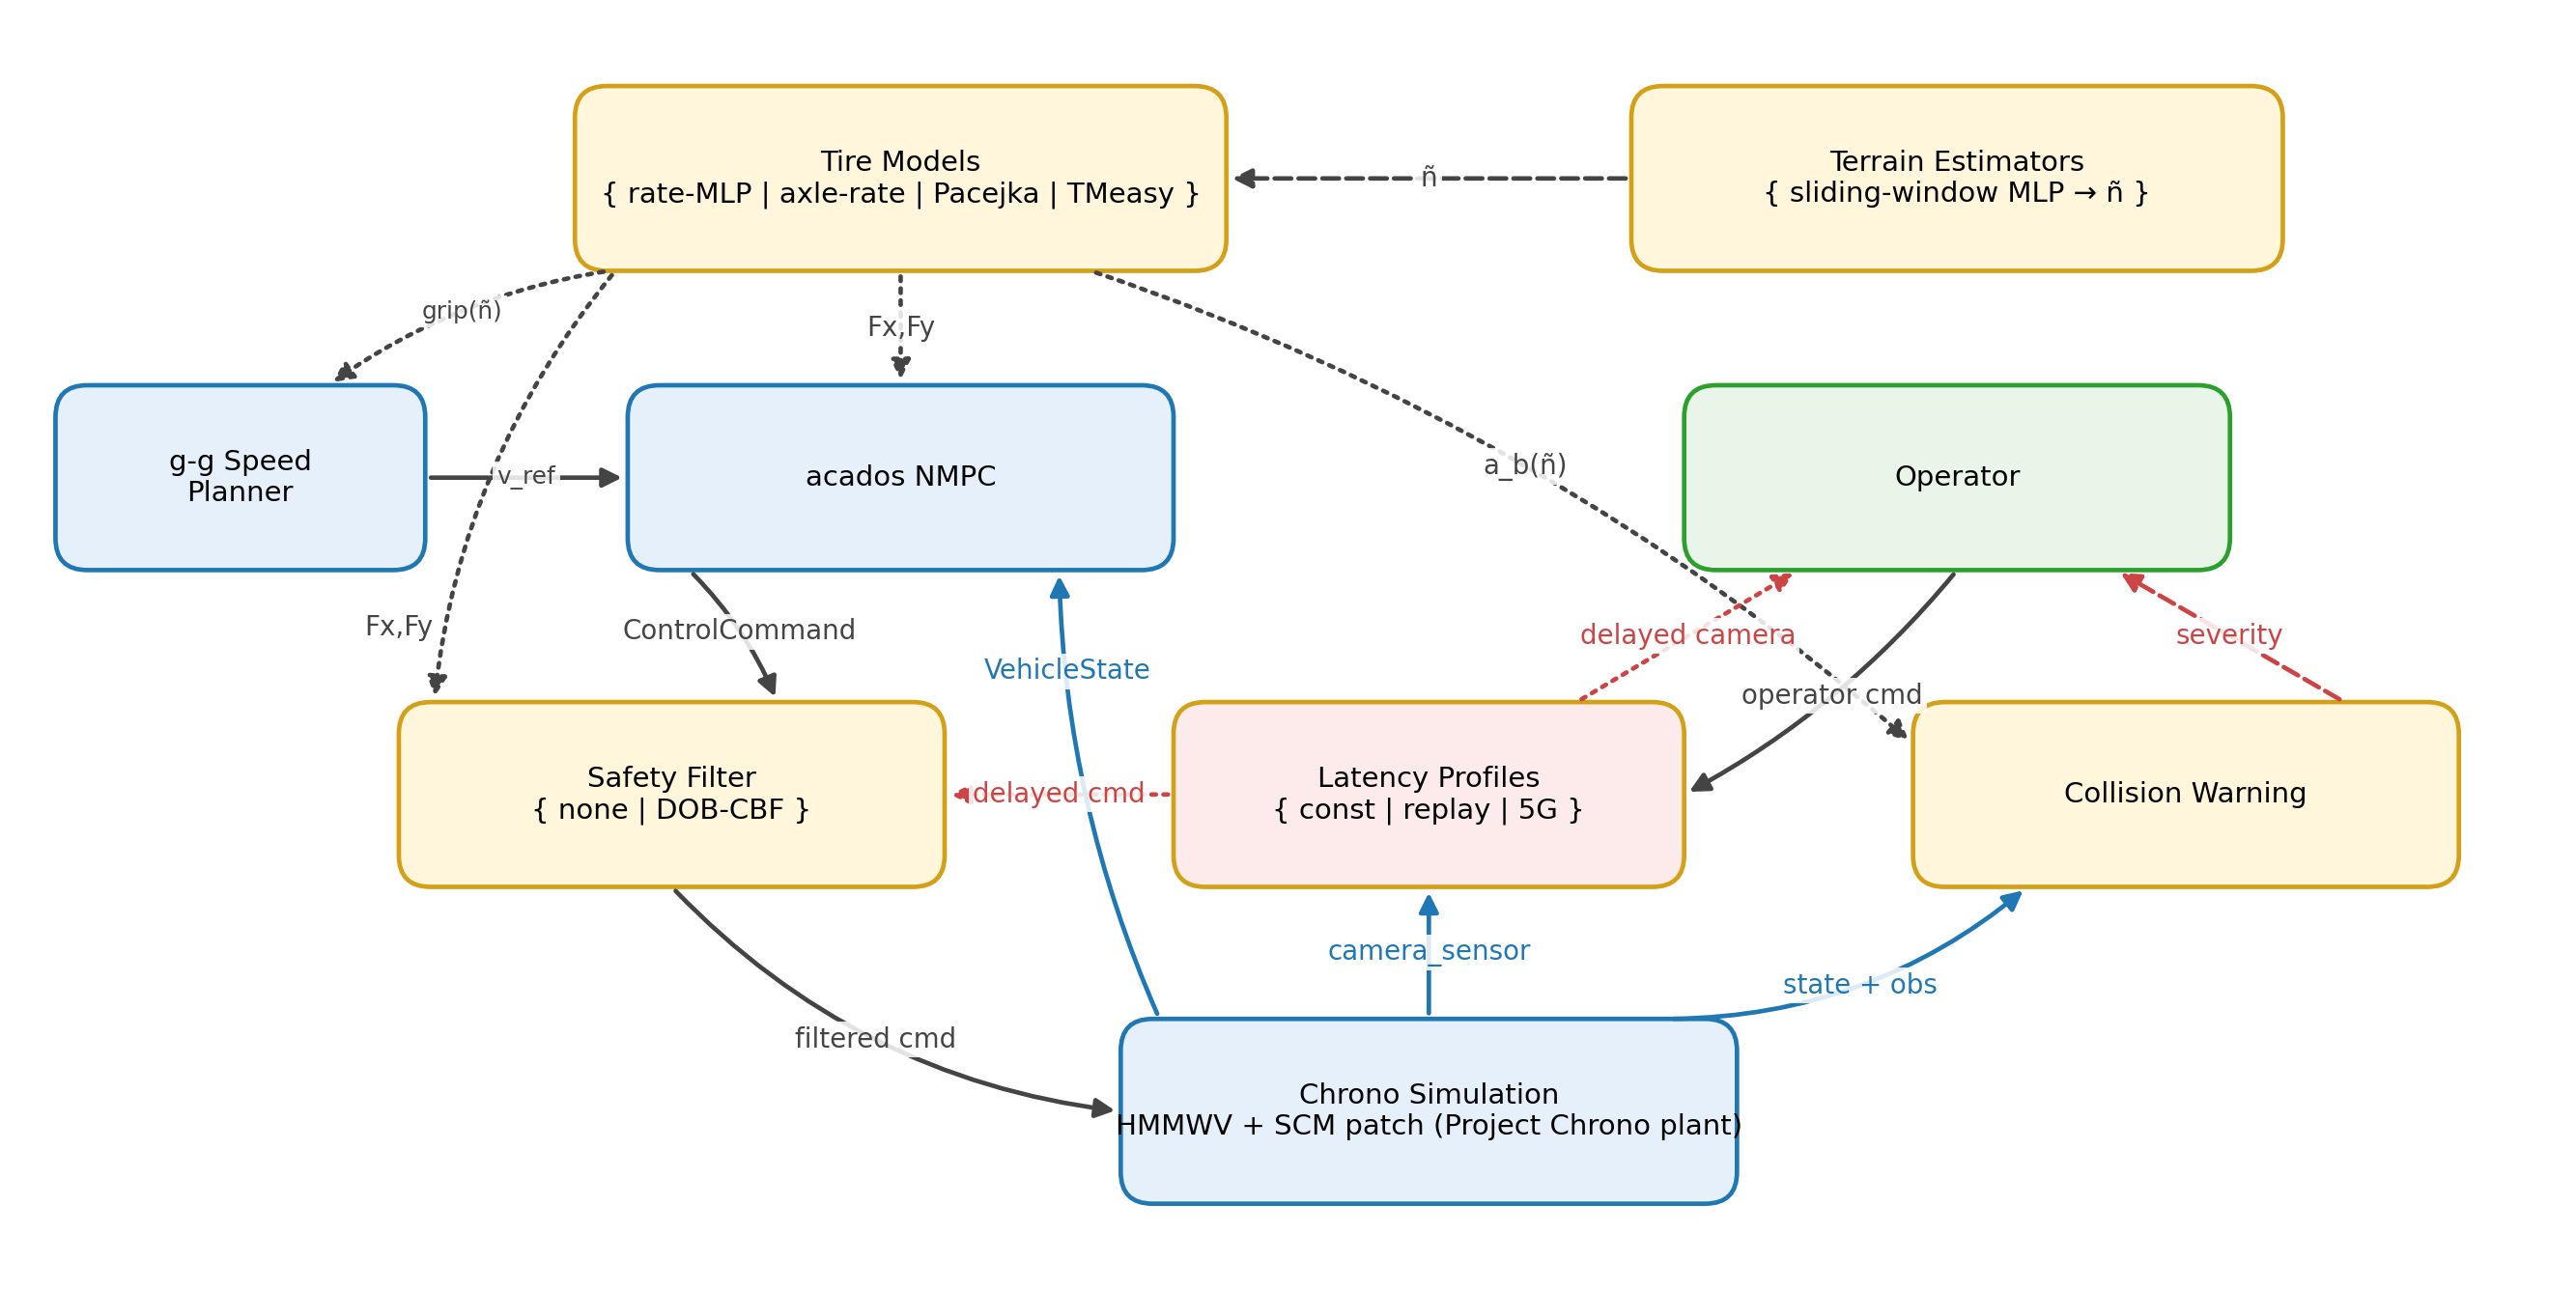
\includegraphics[width=0.92\textwidth]{sys_arch.png}
  \caption{Shared-control framework. Yellow nodes are in-process
    extension points selected by the runtime factories; blue/green nodes
    are process-boundary or operator endpoints. Solid arrows are
    runtime data flow over the ROS~2 / Chrono::ROS transport; dashed arrows are the
    latency-affected operator paths; dotted arrows are tire-surrogate
    queries (build-time CasADi export plus per-tick safety-filter
    rollouts).}
  \label{fig:sysarch}
\end{figure*}

\begin{table}[!t]
  \renewcommand{\arraystretch}{1.15}
  \caption{The six extension points of the framework. Each role is
    defined by one Protocol and has a corresponding registry interface;
    the current runtime conformance test exercises the registry-wired
    safety-filter and collision-warning roles.}
  \label{tab:swap_points}
  \centering
  \scriptsize
  \setlength{\tabcolsep}{3pt}
  \begin{tabular}{@{}lll@{}}
    \toprule
    \textbf{Role} & \textbf{Protocol method} & \textbf{Current variants}\\
    \midrule
    Command source     & \texttt{next\_command}  & NMPC, G29, WASD\\
    Safety filter      & \texttt{filter}         & DOB-CBF; no-filter bypass\\
    Collision warning  & \texttt{evaluate}       & TTC\\
    Tire-force model   & \texttt{predict}        & rate-MLP, axle-rate-MLP,\\
                       &                         & Pacejka, TMeasy\\
    Terrain estimator  & \texttt{observe/estimate} & force+proprioceptive UKF,\\
                       &                         & window-MLP, Bekker/NN-UKF\\
    Latency profile    & \texttt{delay}          & constant, replay, learned 5G\\
    \bottomrule
  \end{tabular}
\end{table}

Both processes pace to wall clock, and the benchmark harness
parallelises across runs, so a single workstation completes the
static-terrain tire benchmark of Section~\ref{sec:tires_static} in
well under an hour.

The split between process-boundary contracts (ROS~2 topics) and
in-process Protocol contracts is deliberate. Any ROS~2 node that
subscribes to the vehicle-state message and publishes the control
command can replace the acados NMPC without touching the simulator,
which is how the tire-model variants of \S\ref{sec:tires} are
evaluated. Human teleoperation reduces to the same normalised steering,
throttle, and brake channels before actuation, so the safety layer
screens autonomous and human commands behind one contract. The forward
collision warning reads the same vehicle-state stream but never writes
to the command path, so it composes with any filter --- including the
no-filter case --- without re-plumbing.

%======================================================================
\section{Differentiable SCM Tire Surrogate}
\label{sec:tires}
%======================================================================

A multilayer perceptron (MLP) maps the tire operating point
$(\kappa,\alpha,F_z,u)$, steering rate, and soil parameters
$\boldsymbol{\theta}_{\mathrm{soil}}\!=\!(K_\phi,K_c,n,c,\phi,k)$
(Bekker--Wong-style rig inputs~\cite{Shibly05}) to longitudinal and
lateral tire forces $(F_x, F_y)$. Where Dallas et
al.~\cite{Dallas21} use a static MLP only, we train three variants:
the static baseline, a \emph{rate-augmented} MLP that adds the
steering rate $\dot\delta$ as an explicit input, and an
\emph{axle-rate} MLP with per-axle rate inputs
$(\dot\delta_f,\dot\delta_r)$. The rate input lets the surrogate
represent the tire force while the operating point is \emph{changing}
--- the transient during fast steering --- rather than only the
quasi-steady force a static map returns; in practice
(Sec.~\ref{sec:tires_rig_vs_vehicle}) this mainly buys robustness
against a transient failure mode rather than a bulk accuracy gain. All
three export as CasADi expressions through which the acados solver
auto-differentiates at every horizon stage.

The paper uses two distinct surrogates. The \emph{tire-rig surrogate}
is trained from controlled single-tire SCM sweeps --- one tire on a
virtual test rig, stepped over a grid of
$(\kappa,\alpha,F_z,\boldsymbol{\theta}_{\mathrm{soil}})$ with the
exact SCM force logged at each operating point (the reproducible
protocol of~\cite{Dallas21}). The \emph{whole-vehicle surrogate} is
trained from closed-loop Chrono::Vehicle HMMWV runs that log each
tire's live operating point alongside the SCM ground-truth force,
capturing the coupled regimes a driven vehicle actually reaches ---
load transfer, yaw, and the body-frame force conventions the isolated
rig never produces. The rig surrogate tests whether the single-tire
learning problem is solvable in isolation; the whole-vehicle surrogate,
deployed for the main NMPC and safety-filter results, tests whether the
controller sees accurate forces in the regimes it drives through.

\subsection{Training data: rig sweeps and closed-loop rollouts}
\label{sec:tires_rig_to_cl}
\label{sec:training_data}

The rig surrogate mirrors the protocol of~\cite{Dallas21}: a single SCM
tire is driven over a Cartesian grid of $(\kappa, \alpha, F_z,
\boldsymbol{\theta}_{\mathrm{soil}})$ and the SCM ground-truth force is
recorded at every operating point. Every label is exact, no closed-loop
feedback confounds the supervision, and the collection parallelises
trivially; the result reaches rig-grid $R^2 \gtrsim 0.95$ on a held-out
rig split and serves as the controlled baseline.

The whole-vehicle surrogate instead targets the controller's deployed
operating distribution, collecting training tuples from the closed-loop
stack itself so the labels carry the high-yaw-rate,
lateral-acceleration, and body-frame force conventions that arise under
aggressive references on deformable soil. A parallel pool of randomised
$(\text{terrain}, \text{path}, \text{speed}, \text{bumpiness},
\text{seed})$ scenarios runs the NMPC against Chrono::Vehicle and logs
the live operating point alongside the SCM force. The deployed surrogate
is trained on \textbf{800 such scenarios}, with the six soil parameters
LHS-sampled jointly over a broad Bekker--Mohr box that \emph{encloses}
the clay, dirt, and sand presets as interior points --- so accuracy on
those terrains is interpolation, not memorisation, and generalisation is
measured on held-out LHS slices and off-manifold soils
(Sec.~\ref{sec:tires_rig_vs_vehicle}) --- together with the maneuver
axes: 264 sand, 270 dirt, 266 clay; 214 sinusoidal, 201 right-left, 200
lane-change, 185 double-lane-change; commanded speeds in
$[3,7]\,\mathrm{m/s}$; bumpiness and rock-count randomised; each scenario
$\sim$10\,s at the controller rate. The aggregated table holds
$\approx 1.85\,\mathrm{M}$ rows of
$(\kappa,\alpha,F_z,u,\dot\delta)\!\to\!(F_x,F_y)$ (front $+$ rear axle
per tick) --- fewer than the rig's $\sim$100k single-tire grid, but drawn
from the distribution the deployed MPC actually visits. Two rig-trained
checkpoints are retained as reproducible rig-static and rig-rate
baselines for the rig-versus-vehicle comparison
(Sec.~\ref{sec:tires_static}).

The NMPC queries the surrogate at each stage. The longitudinal
traction budget $F_x^{\mathrm{trac}}$ is evaluated at reference slip
$\kappa_{\mathrm{ref}}$, $\alpha = 0$, with axle loads $F_z$, speed
$u$, and $\boldsymbol{\theta}_{\mathrm{soil}}$ taken from terrain
presets or the online estimator. Cornering forces $F_y$ use the live
operating point $(\kappa, \alpha, F_z, u)$ at each stage.

The two learned terrain estimators are trained on deliberately
different data, which matters for reading their results. The
sliding-window MLP (Sec.~\ref{sec:estimator}) --- the proprioceptive
channel of the deployed Fused-UKF (Sec.~\ref{sec:ukf}) --- regresses the
Bekker exponent $n$ from a 4\,s window of proprioceptive statistics; it
is trained on 180 LHS soil cells $\times$ 20 scenarios, split between
closed-loop NMPC tracking (sinusoidal / lane-change / right-left at
$\{4,6,8\}\,\mathrm{m/s}$) and scripted open-loop cruise-bias runs, at
bumpiness $\in\{0,4\}$ (the envelope that bounds its in-distribution
claims, Table~\ref{tab:training_data}). The NN-UKF tire surrogate
(Sec.~\ref{sec:ukf}) is trained on 300 scripted sinusoidal-steer runs
with no controller in the loop, half at constant open-loop throttle and
half under a PI cruise loop, over a widened soil box that makes the
canonical presets interior points. Each model therefore sees a different
throttle excitation --- NMPC cruise, none, or a mix --- so its accuracy
is reported only within its own envelope.

\begin{table*}[!t]
  \renewcommand{\arraystretch}{1.15}
  \caption{Training-data provenance for the learned models. ``Loop''
    distinguishes scripted open-loop excitation from closed-loop NMPC
    tracking; bumpiness is the terrain-roughness level present during
    training (and hence the envelope within which each model is
    evaluated).}
  \label{tab:training_data}
  \centering
  \small
  \begin{tabularx}{\textwidth}{@{}L L L c L@{}}
    \toprule
    \textbf{Model (role)} & \textbf{Loop / excitation} & \textbf{Throttle} & \textbf{Bumpiness} & \textbf{Soil / $n$ coverage}\\
    \midrule
    Rig-rate (tire baseline) & open-loop single-tire rig, scripted $\kappa/\alpha$ & --- (fixed rig) & --- & LHS around clay/dirt/sand\\
    Vehicle-rate (deployed NMPC tire) & closed-loop NMPC, 4 paths & NMPC cruise, $[3,7]\,\mathrm{m/s}$ & $\{0,2,4\}$ & full Bekker--Mohr LHS box\\
    Window-MLP (proprioceptive channel of deployed Fused-UKF) & closed-loop NMPC $+$ scripted open-loop & NMPC $+$ cruise-bias & $\{0,4\}$ & $n\in[0.40,1.30]$, 180 LHS cells\\
    NN-UKF tire surrogate (Sec.~\ref{sec:ukf}) & scripted sinusoidal steer, no controller & half const.\ OL / half PI-cruise & $0$ & widened $n\in[0.35,1.35]$\\
    \bottomrule
  \end{tabularx}
\end{table*}

\subsection{Static-terrain benchmark}
\label{sec:tires_static}

The standard MPC is swept over its three deployable tire-force models
(the analytical Pacejka and TMeasy, and the deployed vehicle NN rate-MLP
surrogate) across all
three terrains (clay, dirt, sand), three reference paths (sinusoidal,
lane-change, right-left), three reference speeds
$v_{\mathrm{ref}}\in\{5,7,9\}\,\mathrm{m/s}$, three bumpiness levels,
and five random seeds, for a total of 1215 closed-loop trials. Sensor
noise is enabled in every trial. To keep the comparison fair, the
analytical baselines are \emph{not} run at rigid-road defaults: their
peak lateral friction is calibrated to a single global $\mu=0.42$ by
least-squares fit to the pooled SCM tire-rig forces across the soil box
(the SCM peak $|F_y|/F_z$ ranges from $\approx 0.18$ clay-like to
$\approx 0.47$ sand-like, far below a rigid road), with the
magic-formula and TMeasy shape factors kept at their standard values;
one global set is used for every terrain because the controller has no
per-terrain knowledge. This removes the rigid-road over-grip that
otherwise inflates the baseline error, so the reported gap reflects what
a fixed analytical parameterisation structurally cannot capture, not a
tuning deficit.
Table~\ref{tab:tires_static} reports the mean and standard deviation
of root-mean-square crosstrack error (RMS CTE), speed retention
ratio, and solver wall time across the matrix. The neural row is the
deployed whole-vehicle surrogate; the rig-trained checkpoints are
retained in the benchmark suite as rig-static and rig-rate baselines for
reproducing the rig-to-vehicle comparison. Fig.~\ref{fig:tires_static_heatmap} breaks the same matrix
out per (terrain, path), which makes the analytical-baseline failure
mode at dirt/sinusoidal and dirt/right-left visible at a glance.

\begin{table}[!t]
  \renewcommand{\arraystretch}{1.15}
  \caption{Tire-model benchmark over the full 1215-run matrix (405 runs
    per model), against \emph{SCM-calibrated} analytical baselines
    (single global $\mu\!=\!0.42$, Sec.~\ref{sec:tires_static}). The
    deployed vehicle NN rate-MLP attains the lowest mean RMS CTE,
    $57$--$58\,\%$ below the analytical baselines; the per-model
    \emph{medians} are close ($0.12$--$0.15\,\mathrm{m}$), so the NN's
    gain is in the tail --- the Pacejka and TMeasy rows carry large
    right-skewed standard deviations ($0.49$--$0.53$ vs.\ $0.14$) from
    off-nominal dirt scenarios (Fig.~\ref{fig:tires_static_heatmap})
    that the NN suppresses. All models retain similar speed because
    this controlled comparison fixes the speed reference to the
    geometric curvature profile across every tire model (the deployed
    terrain-aware speed planner of Sec.~\ref{sec:speedplan} is held out
    so the comparison isolates the tracking tire model), so the
    reference, not the tire force model, binds speed here. The NN's higher solve time
    reflects the embedded surrogate evaluation; all three rows remain below the
    $100\,\mathrm{ms}$ controller period.}
  \label{tab:tires_static}
  \centering
  \begin{tabular}{lccc}
    \toprule
    \textbf{Tire model} & \textbf{RMS CTE (m)} & \textbf{Speed} & \textbf{Solve}\\
                         &                       & \textbf{ratio} & \textbf{(ms)}\\
    \midrule
    Pacejka                       & $0.38 \pm 0.49$ & $0.67$ & $4.3$\\
    TMeasy                        & $0.39 \pm 0.53$ & $0.66$ & $4.6$\\
    \textbf{Vehicle NN rate-MLP}  & $\mathbf{0.16 \pm 0.14}$ & $0.67$ & $13.4$\\
    \bottomrule
  \end{tabular}
\end{table}

\begin{figure}[!t]
  \centering
  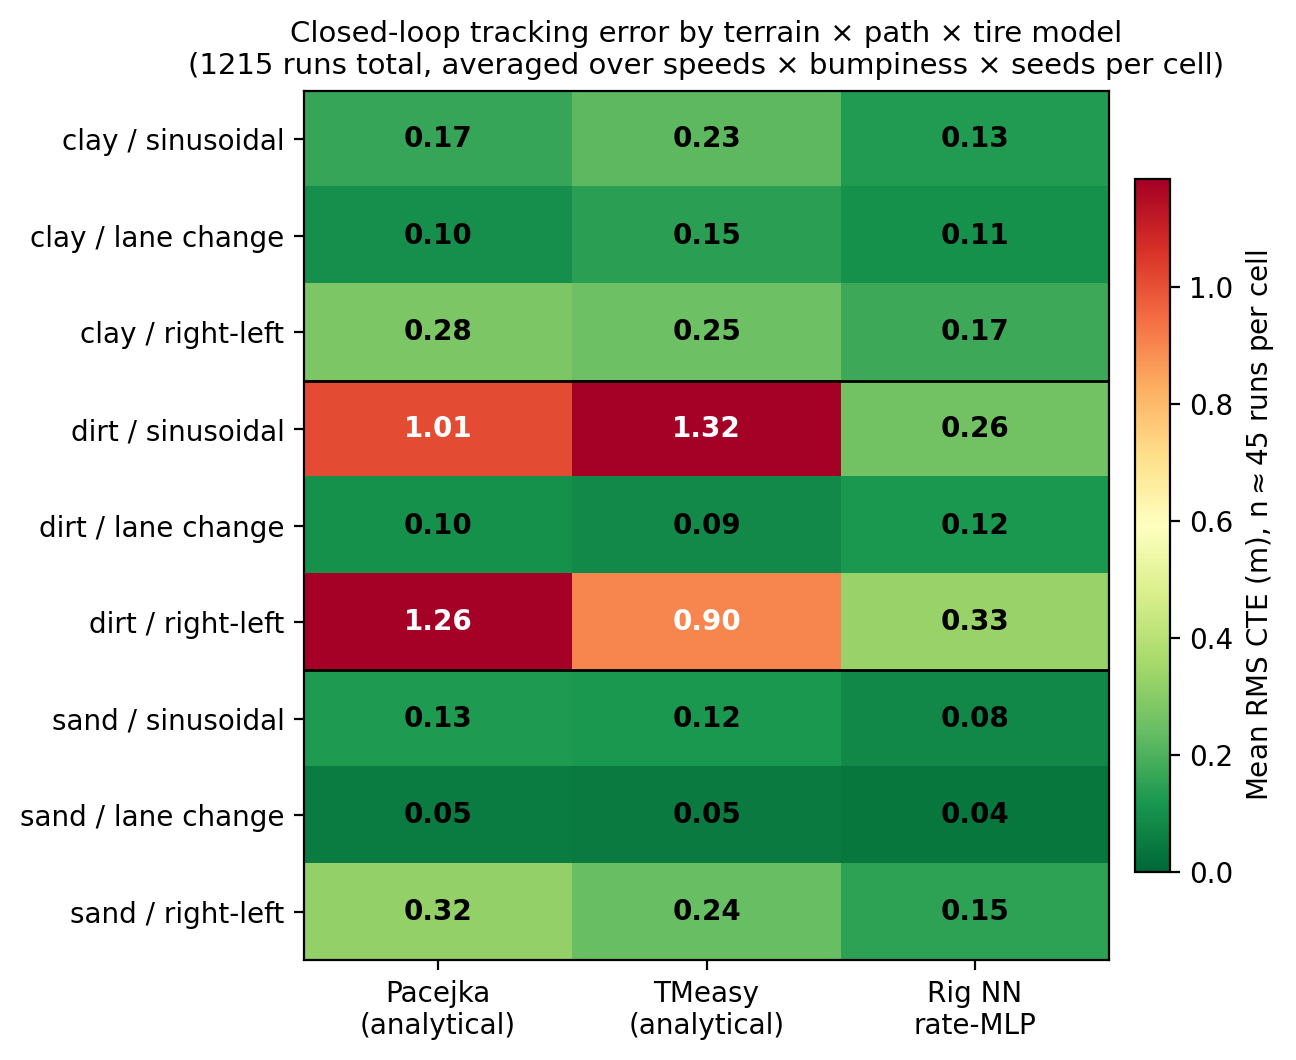
\includegraphics[width=\columnwidth]{cte_master_heatmap.png}
  \caption{Closed-loop RMS CTE per (terrain, path) cell across the
    broader 1215-run sweep (3~speeds $\times$ 3~bumpiness $\times$
    5~seeds per cell). The analytical baselines (Pacejka, TMeasy)
    track well on clay and sand but diverge on dirt/sinusoidal
    ($\sim\!1.0\,\mathrm{m}$) and dirt/right-left
    ($0.9$--$1.2\,\mathrm{m}$), where the curvature-limited reference
    combines with off-nominal sinkage to produce a regime the analytical
    force laws do not cover even after SCM calibration. The Vehicle NN
    rate-MLP suppresses those tails to $0.4$--$0.6\,\mathrm{m}$ while
    matching the calibrated baselines on the benign cells. This per-scenario
    view is what motivates the live-estimator benchmark in
    Sec.~\ref{sec:tires_estimator}.}
  \label{fig:tires_static_heatmap}
\end{figure}

\subsection{Live-estimator-conditioned benchmark}
\label{sec:tires_estimator}

The stronger claim, that the neural surrogate combined with the
online terrain estimator improves tracking over Pacejka and TMeasy,
requires the estimator to update the soil parameters that
the surrogate consumes. The same model set is therefore re-evaluated
with the online estimator enabled, using a 20-second simulation
window with key performance indicators (KPIs) computed after an
8-second post-convergence cutoff.
Table~\ref{tab:tires_estimator} reports the result;
Fig.~\ref{fig:tires_estimator_heatmap} shows the per-scenario
heatmap. Because this regime conditions on the live estimator (not the
static terrain prior of Table~\ref{tab:tires_static}) and reports
\emph{medians} over the larger 1620-run matrix, its analytical-baseline
numbers are not directly comparable to Table~\ref{tab:tires_static}'s
mean$\pm$std over the 1215-run static matrix; the two report the
static-prior and live-estimator regimes respectively.

Two points frame Table~\ref{tab:tires_estimator}. First, the static
neural row is conditioned on the matched terrain preset and behaves as a
near-oracle reference, whereas the $+$estimator row recovers the soil
parameters online from inertial and wheel-speed signals alone. The
estimator variant nearly matches that near-oracle row (median $0.177$
vs.\ $0.174\,\mathrm{m}$; the $95\,\%$ bootstrap intervals,
$[0.150,0.191]$ and $[0.142,0.191]\,\mathrm{m}$, overlap) with no prior
terrain knowledge, and both NN rows reduce median RMS CTE by
$39$--$41\,\%$ against the SCM-calibrated Pacejka and TMeasy baselines.
The deployable claim is thus that the estimator recovers most of the
oracle-prior benefit without the prior, not that it beats a correct
prior. Second, the per-row distributions are right-skewed by a few
high-error scenarios (mostly Pacejka and TMeasy on dirt at
$v_{\mathrm{ref}}\!=\!7\,\mathrm{m/s}$, where the analytical baselines
collide with the curvature limit); Fig.~\ref{fig:tires_estimator_heatmap}
shows the full distribution.

\begin{table}[!t]
  \renewcommand{\arraystretch}{1.15}
  \caption{Live-estimator-conditioned tire-model benchmark, full
    1620-run scheduled matrix (405 per variant), KPI window from
    $t=8\,\mathrm{s}$.
    Values are \emph{median} RMS CTE: the per-variant distributions are
    strongly right-skewed by a few high-error dirt scenarios
    (Fig.~\ref{fig:tires_estimator_heatmap}), so the median is the
    representative statistic. The static neural row is
    conditioned on the matched terrain preset (near-oracle); the
    $+$estimator row runs the deployed force+proprioceptive
    Fused-UKF (Sec.~\ref{sec:ukf}) online. Per terrain the estimator
    matches the oracle on dirt and sand (median gap $\le\!1\,\mathrm{cm}$)
    and retains a residual gap only on clay (median $0.40$ vs.\
    $0.21\,\mathrm{m}$), where online $n$-estimation on soft, low-$n$ soil
    is hardest; the pooled CTE column blends these three. Both NN rows
    reduce median RMS CTE by $39$--$55\,\%$ relative to the
    \emph{SCM-calibrated} analytical baselines (single global $\mu\!=\!0.42$).}
  \label{tab:tires_estimator}
  \centering
  \setlength{\tabcolsep}{4pt}
  \begin{tabular}{lccc}
    \toprule
    \textbf{Variant} & \textbf{CTE (m)} & \textbf{vs.\ Pacejka} & \textbf{vs.\ TMeasy}\\
    \midrule
    Pacejka (static)            & $0.29$ & ---       & ---\\
    TMeasy (static)             & $0.28$ & ---       & ---\\
    NN rate-MLP (static)        & $0.13$ & $-55\,\%$ & $-53\,\%$\\
    \textbf{NN rate-MLP $+$ estimator} & $\mathbf{0.17}$ & $\mathbf{-41\,\%}$ & $\mathbf{-39\,\%}$\\
    \bottomrule
  \end{tabular}
\end{table}

A separate ablation isolates the deployable value of the estimator
explicitly. Holding the controller's static terrain prior at dirt
regardless of the plant terrain gives the
wrong-prior baseline, comparable directly against the matched-prior
oracle and the estimator-on variant on the same matrix
(clay$+$sand $\times$ sinusoidal $\times$ $v\in\{5,7\}\,\mathrm{m/s}$
$\times$ flat terrain $\times$ $5$ seeds, $20$ runs per variant).
Table~\ref{tab:wrong_prior} reports the result. On clay the wrong
dirt prior gives RMS CTE $1.53\,\mathrm{m}$, the estimator-on variant
(the deployed Fused-UKF, Sec.~\ref{sec:ukf}) adapts from the same dirt
initialisation and recovers to $0.63\,\mathrm{m}$, close to the
matched-prior oracle ($0.49\,\mathrm{m}$) -- the estimator closes
$\approx 86\,\%$ of the prior-mismatch gap on the harder terrain.

\begin{table}[!t]
  \renewcommand{\arraystretch}{1.10}
  \caption{Wrong-prior ablation: RMS CTE (m) when the controller's
    static terrain prior is fixed to dirt regardless of plant terrain,
    compared against the matched-prior near-oracle and the estimator-on
    variant. $60$ runs total ($20$ per variant). The matrix excludes
    dirt (where the dirt-prior is by construction matched) and the
    other paths/bumpiness levels of Table~\ref{tab:tires_estimator};
    absolute numbers are therefore not comparable across the two
    tables. The estimator nearly recovers the matched-prior
    performance from a wrong initialisation on clay; matched and
    wrong priors both yield low error on sand because dirt is closer to sand
    than to clay on the soil-parameter manifold.}
  \label{tab:wrong_prior}
  \centering
  \begin{tabular}{lccc}
    \toprule
    \textbf{Variant} & \textbf{Clay} & \textbf{Sand} & \textbf{Mean}\\
    \midrule
    Matched static prior (oracle) & $0.486$ & $0.056$ & $0.271$\\
    Wrong (dirt) static prior     & $1.528$ & $0.061$ & $0.794$\\
    \textbf{Estimator-on (dirt $\to$ adapt)} & $\mathbf{0.632}$ & $\mathbf{0.059}$ & $\mathbf{0.346}$\\
    \bottomrule
  \end{tabular}
\end{table}

\begin{figure}[!t]
  \centering
  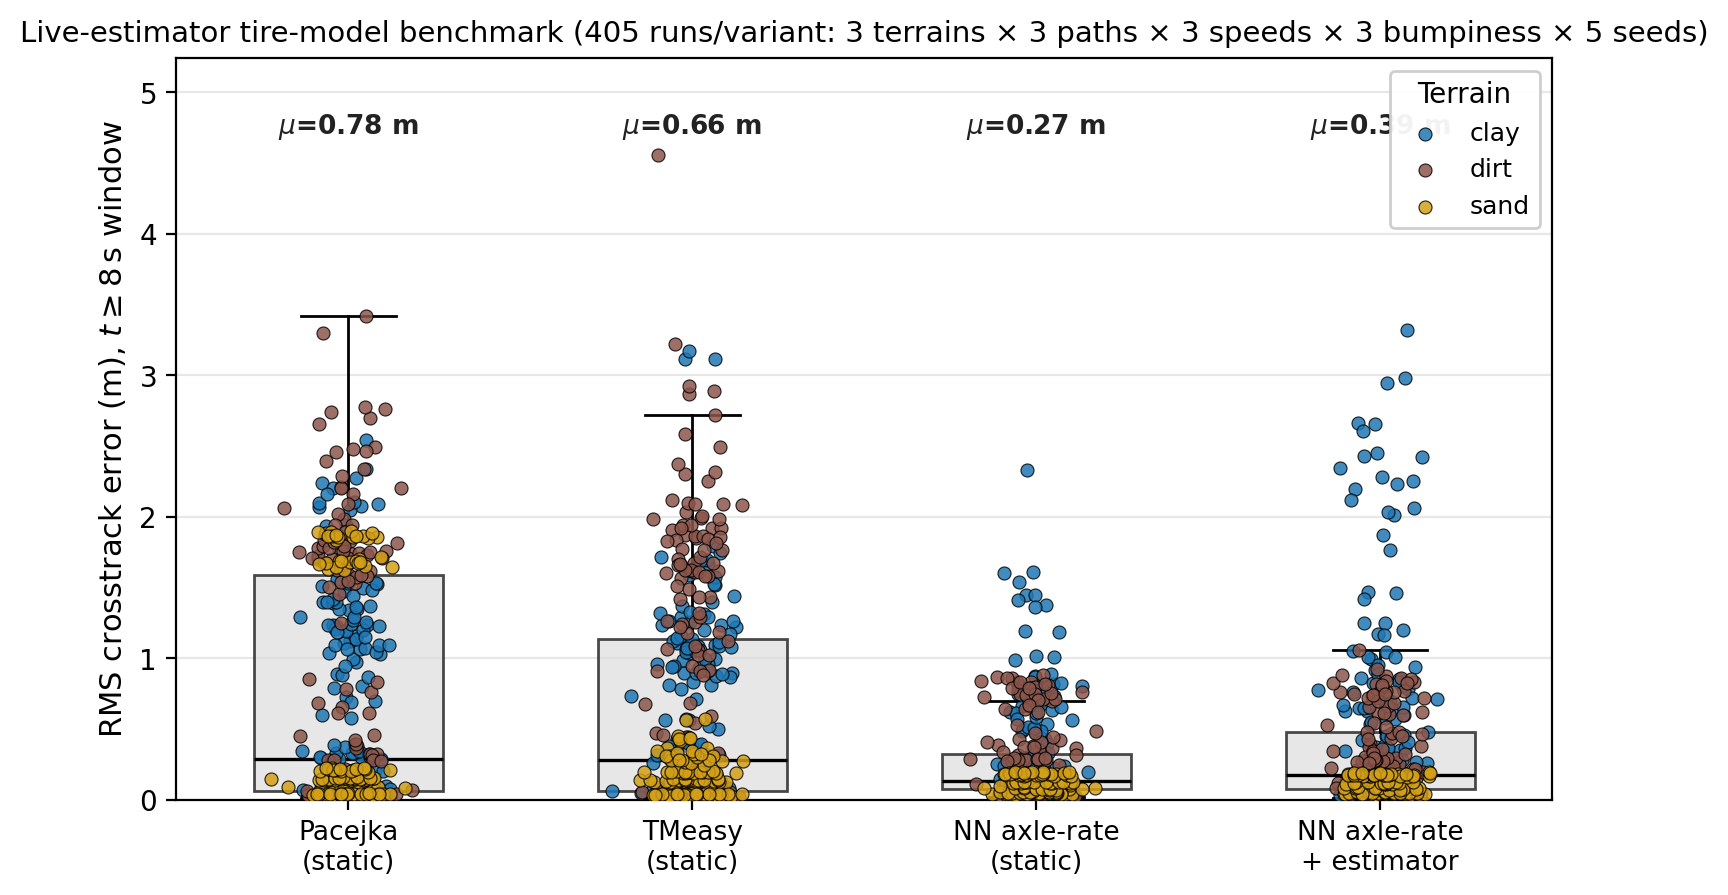
\includegraphics[width=\columnwidth]{tire_model_with_estimator_rms_cte_heatmap.png}
  \caption{Same benchmark, RMS CTE distribution per variant.
    Box plots show interquartile range and median across the valid KPI
    rows from the 405 scheduled runs per variant; jittered scatter
    points are coloured by terrain
    (clay, dirt, sand). The two analytical baselines (Pacejka, TMeasy)
    carry long right tails driven by a few dirt cases at higher
    $v_{\mathrm{ref}}$; both neural variants substantially compress the distribution
    tail. The estimator-on variant nearly matches the matched-prior
    static row, the deployable claim of Sec.~\ref{sec:tires_estimator}.}
  \label{fig:tires_estimator_heatmap}
\end{figure}

\subsection{Controlled rig-versus-whole-vehicle comparison}
\label{sec:tires_rig_vs_vehicle}

The rig-vs-whole-vehicle question motivating
Sec.~\ref{sec:tires_rig_to_cl} is settled by a controlled retrain
that removes two confounds present in the earlier comparison: rig
checkpoints used smaller MLPs (16-4, 16-8) than vehicle checkpoints
(32-16), and the vehicle training set jittered scenarios around the
three canonical deployment terrains rather than sampling broadly. We
retrain:

\begin{itemize}
\item three rig checkpoints (32-16 static, 32-16 rate, 64-32 rate) on
  the existing 100k single-tire SCM CSVs;
\item three whole-vehicle checkpoints (matched architectures) on a
  fresh 800-scenario closed-loop dataset that LHS-samples
  $\boldsymbol\theta_{\mathrm{soil}}$ across the same Bekker--Mohr box
  the rig uses (no canonical-preset jitter).
\end{itemize}

Offline force prediction on a held-out LHS test slice exposes a
generalisation gap the canonical-jitter eval set hides: a
canonical-jitter-trained whole-vehicle checkpoint's $R^2(F_y)$ drops from
$+0.58$ on canonical-jitter data to $-0.30$ on LHS-terrain data,
while the LHS-trained MLPs hold $R^2 \approx 0.71$ on both
eval sets. The LHS-trained vehicle MLPs are not better at predicting
in-distribution data; the canonical-jitter-trained MLPs over-fit the
deployment-terrain neighbourhood.

The controlled closed-loop tire-model sweep (432 runs, 6 surrogates
$\times$ 3 terrains $\times$ 3 paths $\times$ 2 speeds $\times$ 2
bumpiness $\times$ 2 seeds; planner-only, sensor noise on) is
summarised in Table~\ref{tab:tires_rig_vs_vehicle}. The pre-retrain
rig-trained advantage narrows substantially
(Fig.~\ref{fig:rig_vs_vehicle_paired}):

\begin{itemize}
\item Static MLPs: the rig surrogate remains decisively better
  ($0.090\,\mathrm{m}$ vs $0.116\,\mathrm{m}$, 20\,\%).
\item Rate MLPs (32-16): rig and vehicle match
  ($0.090$ vs $0.091\,\mathrm{m}$).
\item Rate MLPs (64-32): tied within noise
  ($0.100$ vs $0.105\,\mathrm{m}$).
\end{itemize}

Per-tick force-prediction smoothness explains the shrinking gap:
aggregated over the 432 runs, the LHS-trained vehicle surrogates have
$\mathrm{std}(\dot F_y^{\mathrm{pred}})$ around $16$-$20$~kN/s, much
closer to the rig surrogates' $14$~kN/s (the $32$-$16$ rig-rate
variant) than the canonical-jitter-trained vehicle MLPs' $40$~kN/s. Wider
training-terrain coverage acts as an effective low-pass on the
closed-loop SCM signal in the same way LHS-independent sampling did
for the rig.

\begin{table}[!t]
  \renewcommand{\arraystretch}{1.15}
  \caption{Controlled rig-vs-whole-vehicle sweep (432 closed-loop
    runs, planner-only, sensor noise on). Matched architecture in
    each pair; rig retrains use the kept 100k LHS rig CSV, vehicle
    retrains use a fresh 800-scenario LHS-terrain closed-loop dataset.
    The earlier small-capacity rig and vehicle checkpoints are
    preserved in the benchmark suite for reproducibility.}
  \label{tab:tires_rig_vs_vehicle}
  \centering
  \footnotesize
  \begin{tabular}{lccc}
    \toprule
    \textbf{Surrogate (32-16 / 64-32 paired)} & \textbf{RMS CTE} & \textbf{Speed} & \textbf{Solve}\\
                                              & \textbf{(m)} & \textbf{ratio} & \textbf{(ms)}\\
    \midrule
    Rig static (32-16)        & $\mathbf{0.090}$ & $0.73$ & $7.5$\\
    Vehicle static (32-16)    & $0.116$          & $0.73$ & $7.5$\\
    Rig rate (32-16)          & $0.090$          & $0.73$ & $9.7$\\
    Vehicle rate (32-16)      & $0.091$          & $0.73$ & $9.7$\\
    Rig rate (64-32)          & $0.100$          & $0.73$ & $13.6$\\
    Vehicle rate (64-32)      & $0.105$          & $0.73$ & $13.7$\\
    \bottomrule
  \end{tabular}
\end{table}

\begin{figure}[!t]
  \centering
  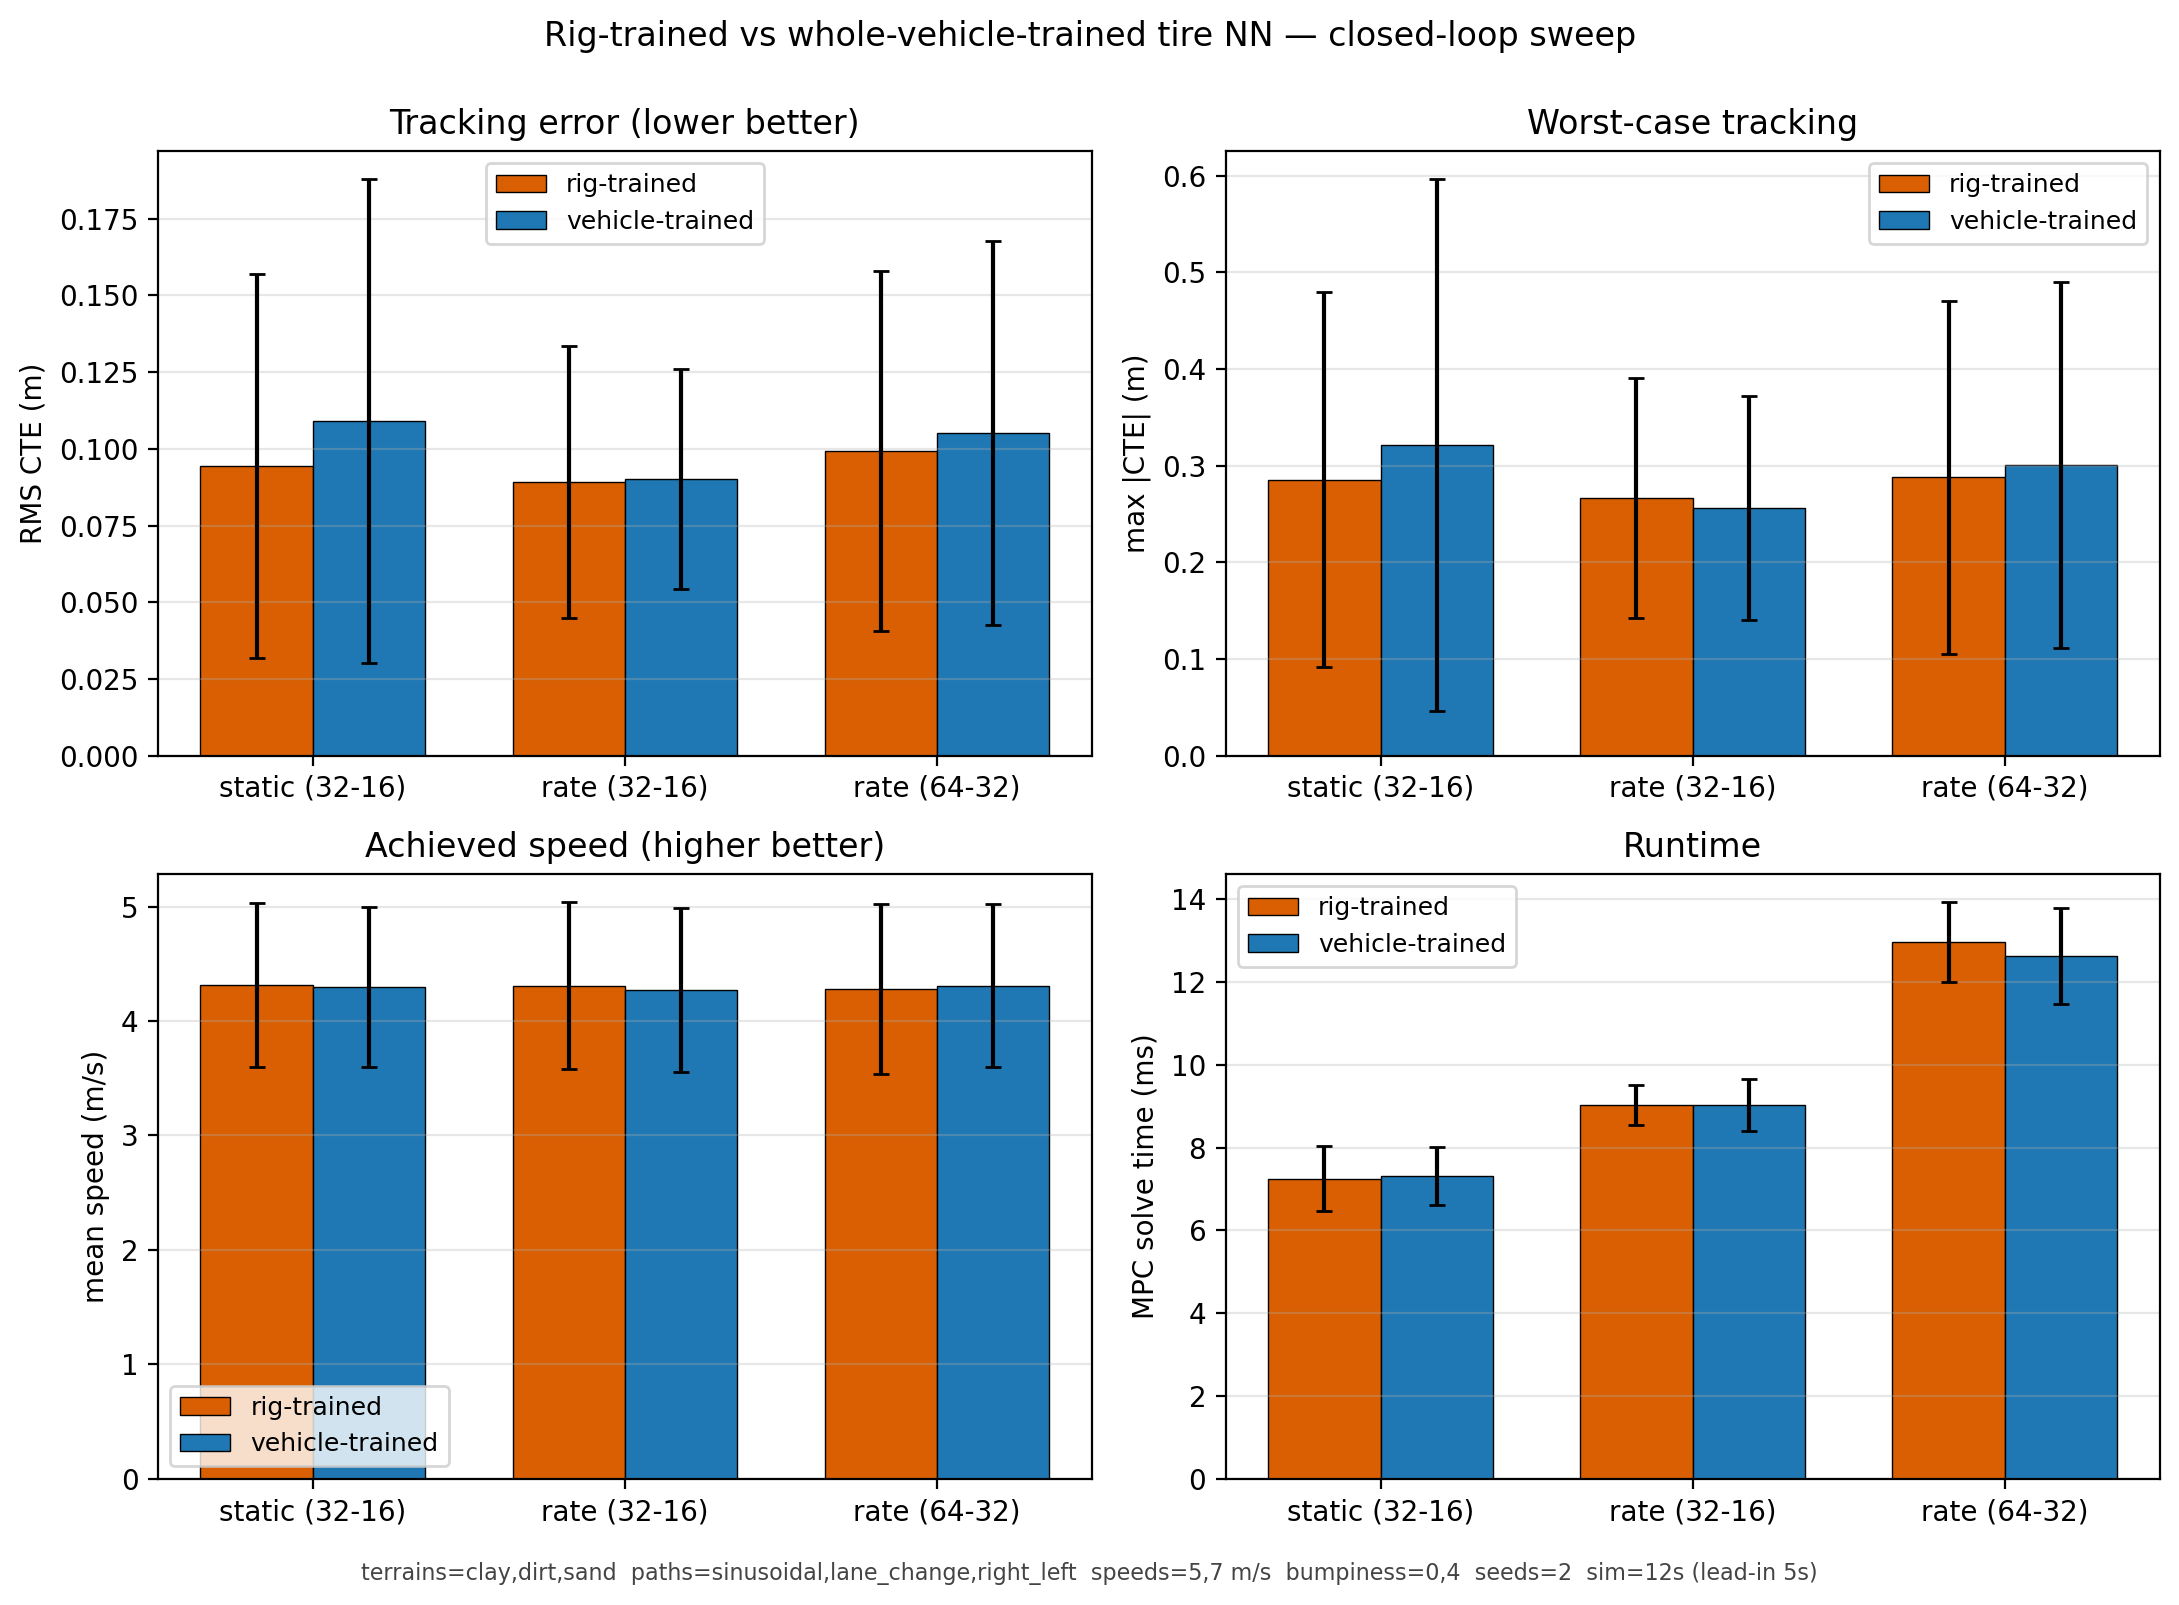
\includegraphics[width=\columnwidth]{rig_vs_vehicle_paired_bars_v2.png}
  \caption{Aggregate metrics over the 432-run controlled sweep, six
    surrogates paired by architecture and signature. RMS CTE,
    worst-case $|\mathrm{CTE}|$, achieved speed, and solver wall time
    on the same matrix. Bars are mean $\pm$ s.d.~across 72 cells per
    surrogate. The pre-retrain rig-trained advantage narrows
    to a static-only effect once architecture is matched and the
    whole-vehicle training data is LHS-sampled over the same Bekker--
    Mohr box the rig uses.}
  \label{fig:rig_vs_vehicle_paired}
\end{figure}

\paragraph{Force accuracy and closed-loop tracking are different metrics}
The CTE numbers in Table~\ref{tab:tires_rig_vs_vehicle} are within
1\,cm of each other across the four mid-size variants. To see what
each surrogate is doing during those runs, we replay all four on twelve
logged trajectories (one shown in Fig.~\ref{fig:rig_vs_vehicle_4way}),
computing per-tick front-axle $|\Delta F_y|$ against the Chrono ground
truth without re-running the simulator. Mean RMSE across the twelve
scenarios:

\begin{center}\footnotesize
\setlength{\tabcolsep}{4pt}
\begin{tabular}{@{}lc@{}}
\textbf{Surrogate}                            & \textbf{Mean RMSE $F_y$ (N)} \\ \midrule
Rig static (32-16)                            & $632$ \\
Vehicle static (32-16)                        & $645$ \\
Rig rate (64-32)                              & $671$ \\
Vehicle rate (64-32, deployed)                & $706$ \\
Ensemble (0.4 rig + 0.6 vehicle, rate)        & $637$ \\
\end{tabular}
\end{center}

The deployed vehicle-rate surrogate is the \emph{worst} of the four on
force-RMSE, yet the most reliable in closed loop. Driving the standard
MPC with each surrogate over six scenarios, the static and rate vehicle
surrogates stay within $5\,\mathrm{cm}$ on five of six, but the static
surrogate suffers a catastrophic failure on clay/right-left at
$v_{\mathrm{ref}}=7\,\mathrm{m/s}$ ($1.07\,\mathrm{m}$ RMS CTE against
the rate variant's $0.16\,\mathrm{m}$); mean CTE is $0.18\,\mathrm{m}$
(rate) versus $0.33\,\mathrm{m}$ (static), matching at
$0.185\,\mathrm{m}$ once that case is excluded. The rate variant's
smoother, lower-amplitude $F_y$ trace under-predicts transient peaks but
avoids the static checkpoint's failure mode, which is why it is deployed
despite the higher force-RMSE. A $w=0.4$ rig-plus-vehicle ensemble
cancels the opposing biases at zero deployment cost ($637\,\mathrm{N}$,
$5\,\%$ better than vehicle alone) and is the recommended default for
downstream consumers such as the safety filter and the
collision-warning braking budget.

\begin{figure}[!t]
  \centering
  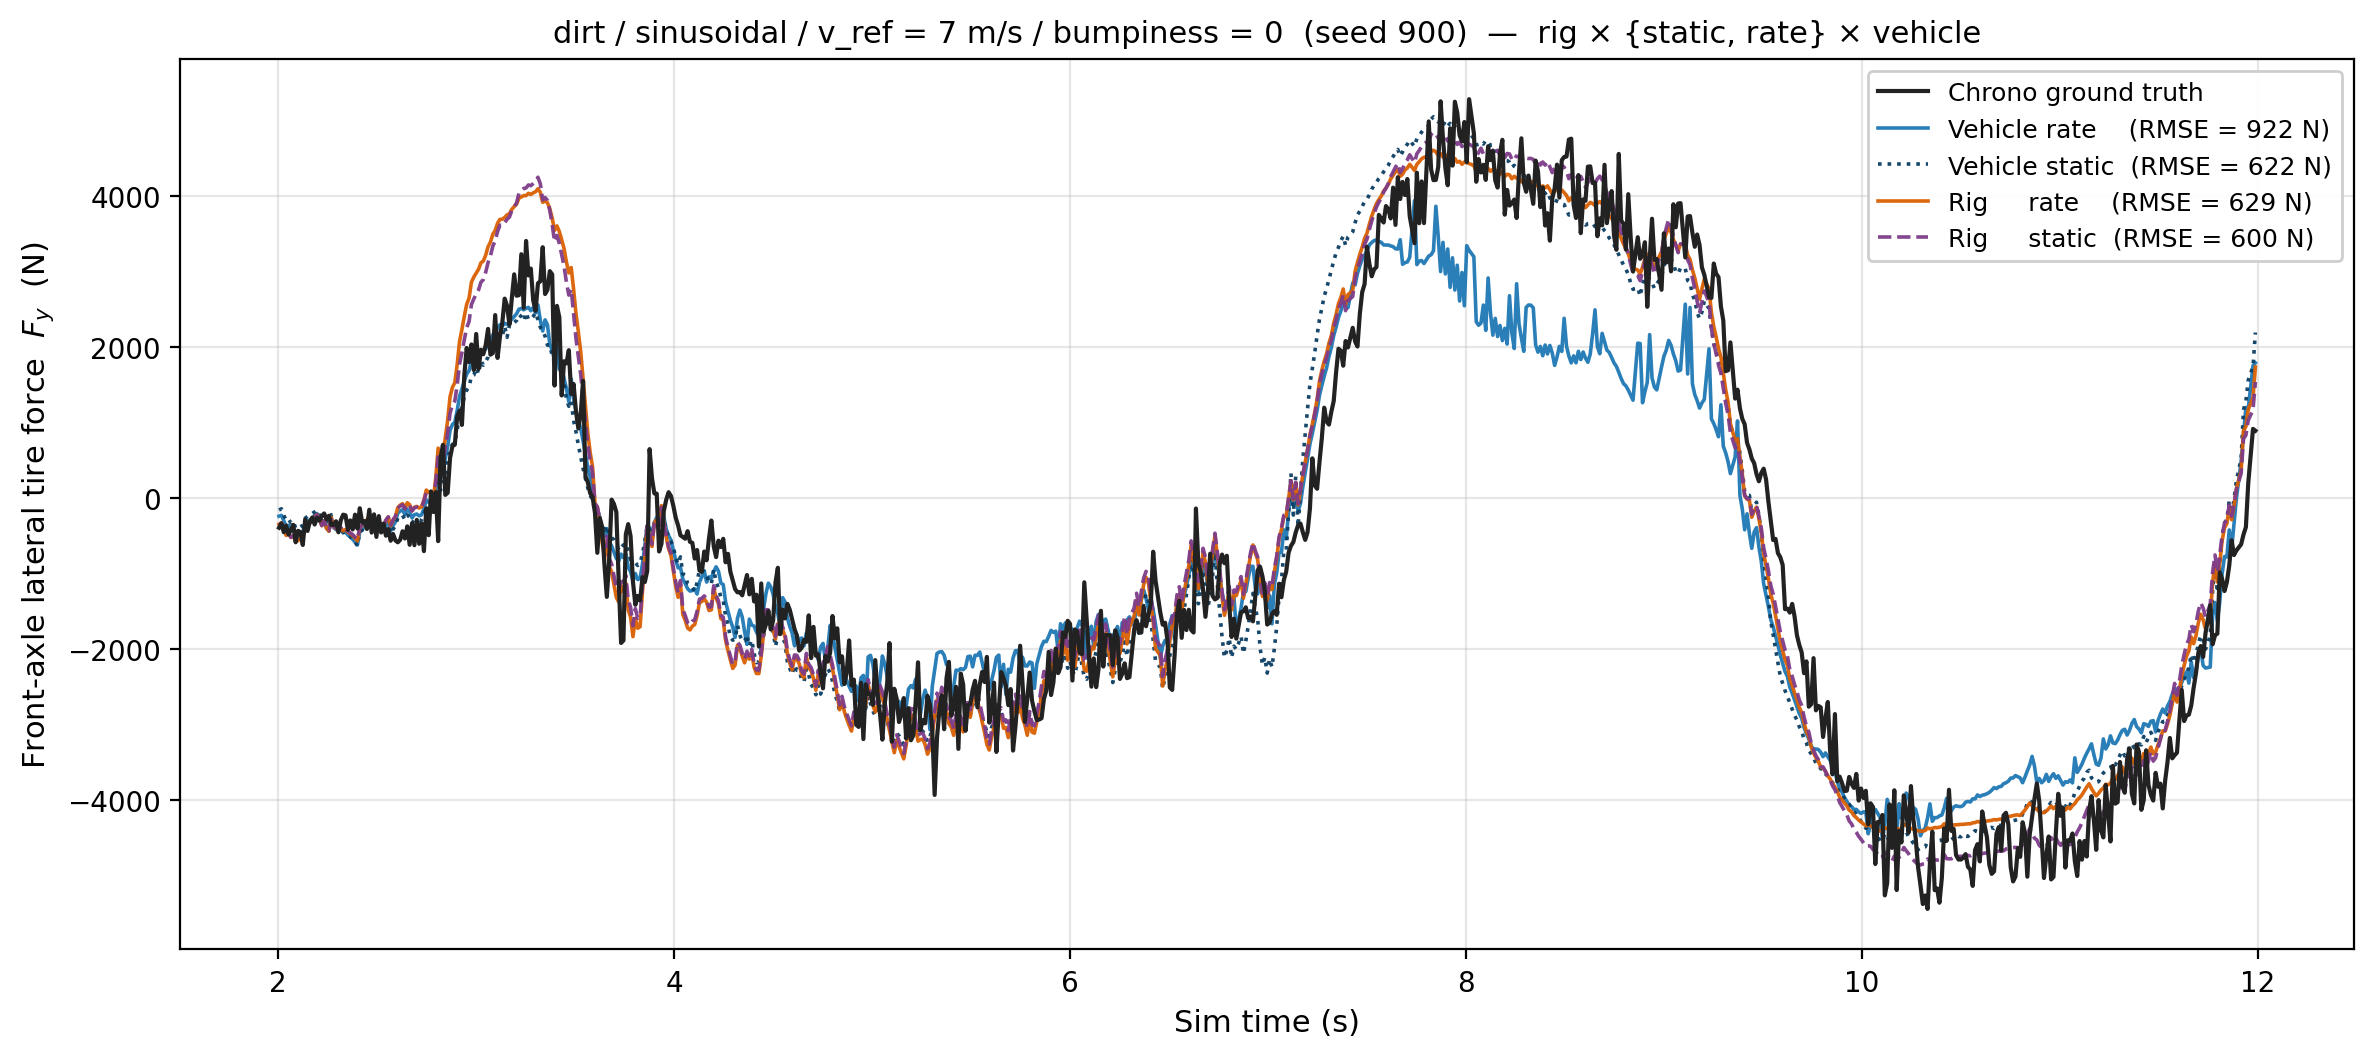
\includegraphics[width=\columnwidth]{fig1_force_4way_dirt_sinusoidal_v7_b0_s900.png}
  \caption{One representative scenario from the four-way comparison
    (dirt, sinusoidal, $v_{\mathrm{ref}}=7\,\mathrm{m/s}$, $b=0$),
    front-axle $F_y$. Black is Chrono ground truth; the four
    coloured traces are the deployed vehicle rate surrogate (light
    blue), the vehicle static surrogate (dark blue dotted),
    rig rate (orange), and rig static (purple dashed). Vehicle rate
    consistently under-predicts the peaks; the rig variants
    over-predict the same peaks; both static checkpoints track the
    envelope most tightly. The deployed default still attains the lowest RMS
    CTE but at the cost of the largest force-RMSE.}
  \label{fig:rig_vs_vehicle_4way}
\end{figure}

The takeaway for deployment: the whole-vehicle pipeline is the right
default \emph{when the training data is LHS-sampled across the same
operating-point box the rig spans}. Training on the LHS-terrain
dataset rather than canonical-preset jitter closes the
generalisation gap the rig pipeline exposes; the
default DOB-CBF safety filter, which reads the surrogate as a static
traction-ceiling query, pairs cleanly with either surrogate. The full
retrain log -- the offline force-prediction tables on both evaluation
sets and the complete smoothness aggregation -- is omitted here for
space.

\subsection{Open-loop prediction validation}
\label{sec:pred_validation}
The closed-loop CTE results establish that the surrogate is accurate
enough to control with, but not whether the NMPC's internal predictions
match the plant --- the property an MPC relies on. We validate
this directly: the controller logs its full predicted horizon trajectory
($4\,$s at $0.1\,$s stages) at every solve, and we compare the predicted
state at each horizon stage against the actual Chrono trajectory that
many steps later, aggregated over $18$ runs (clay/dirt/sand $\times$
sinusoidal $\times\,v\!\in\!\{5,7\}\,$m/s $\times$ 3 seeds, deployed
vehicle-rate surrogate). Fig.~\ref{fig:pred_validation} overlays the
controller's predicted horizons directly on the actual plant trace for a
representative firm-sand run; the per-terrain drift magnitudes quoted
below are means over the full matrix.

The NMPC predicts the \emph{path geometry} accurately --- heading drift
stays below $0.15\,$rad over the full $4\,$s horizon on every terrain ---
but \emph{over-predicts longitudinal speed} by ${\approx}0.5\,$m/s almost
immediately, growing to ${\approx}1.0\,$m/s by $4\,$s on firm sand. The
position drift (up to $2.7\,$m at $4\,$s) is therefore dominated by
accumulated speed error, not lateral error. The prediction weakness is
concentrated in the longitudinal channel, and a signed analysis shows
the bias is \emph{terrain-dependent}: firm soil over-predicts speed,
soft dirt under-predicts, and clay is accurate. It reflects the
kinematic longitudinal model ($\dot u\!=\!a_x$) omitting a
terrain-varying motion-resistance term --- not a tire-surrogate feature
deficit, since the surrogate $F_x$ is not used in the longitudinal
channel (Sec.~\ref{sec:feature_headroom}). The throttle disturbance
observer (Sec.~\ref{sec:throttledob}) closes this gap online and the
$10\,$Hz re-planning masks it in closed loop; the lateral ($F_y$)
channel is already accurate.

\begin{figure*}[!t]
  \centering
  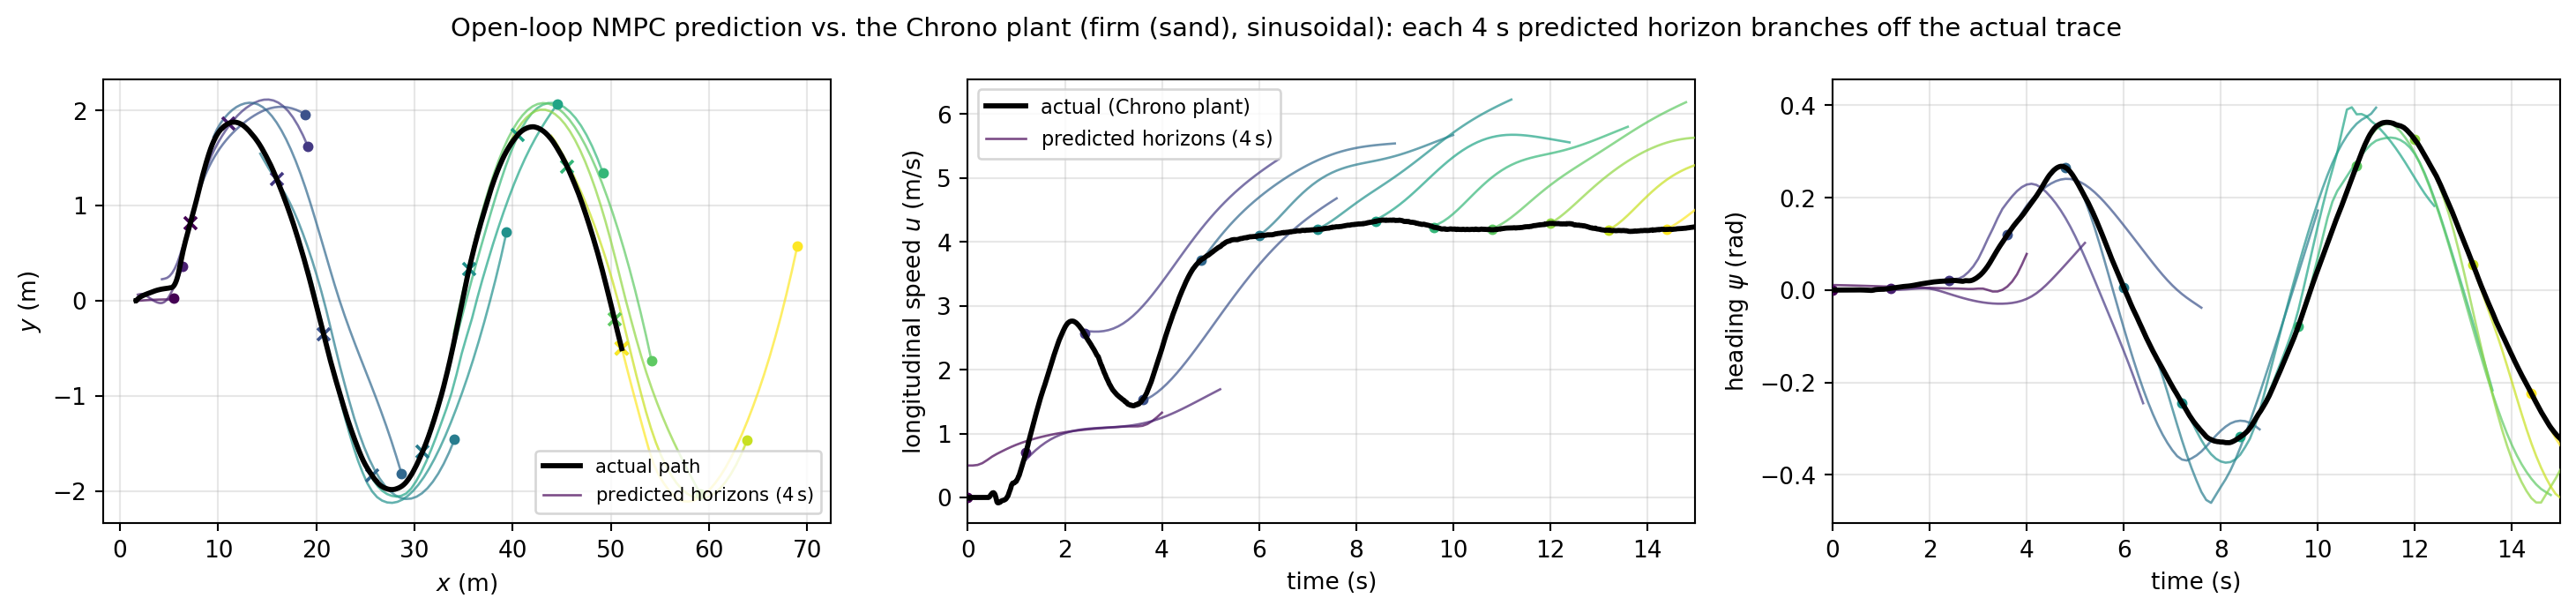
\includegraphics[width=\textwidth]{rollout_prediction_validation.png}
  \caption{Open-loop NMPC prediction versus the Chrono plant for a
    representative firm-sand sinusoidal run (deployed vehicle-rate
    surrogate). Each $4\,$s predicted horizon (thin, colour-graded by
    launch time) branches off the actual plant trace (bold black).
    \textbf{Left ($x$--$y$ path):} the predicted horizons trace the
    actual path --- the geometry is predicted well --- but on firm sand
    the over-predicted speed carries each predicted endpoint (filled
    dot) \emph{ahead} of the vehicle's actual position at the same
    instant (cross): the along-track position drift (${\approx}2.7\,$m
    by $4\,$s). \textbf{Middle (speed $u$):} the horizons run
    \emph{above} the plant and the gap widens along the horizon --- the
    $F_x$ motion-resistance bias the throttle disturbance observer
    absorbs online. \textbf{Right (heading $\psi$):} the horizons hug
    the plant, confirming the lateral ($F_y$) channel is accurate.
    Aggregate drifts across the 18-run matrix are quoted in the text
    ($\le 0.15\,$rad heading over $4\,$s; position drift dominated by
    the longitudinal speed bias, not lateral error).}
  \label{fig:pred_validation}
\end{figure*}

\subsection{Feature headroom and the structural force-prediction floor}
\label{sec:feature_headroom}
Section~\ref{sec:pred_validation} isolates $F_x$ as the dominant
prediction error. Two prediction weaknesses remain to test: this
longitudinal $F_x$ bias, and the rear-axle $F_y$, which the deployed
surrogate predicts least accurately of the four force channels. We ask
whether either is closable with additional \emph{causal, MPC-available}
features. Holding the deployed per-axle architecture fixed
($64\!\times\!32$ tanh, scenario split, three seeds), we retrain with
progressively richer inputs --- body-frame lateral velocity $v$, yaw
rate $\omega$, road-wheel angle $\delta$, a kinematic
lateral-load-transfer estimate, and their first differences --- and
report held-out RMSE per axle (Table~\ref{tab:feature_headroom}). The
candidates are confined to causal state the MPC already carries; body
accelerations are excluded, since $a=\Sigma F/m$ makes them the labels
themselves.

The response is strongly asymmetric. Front-axle lateral force improves by
$14\%$ once the dynamic state and its rates are supplied: $F_{y,f}$
genuinely benefits from richer vehicle context. The longitudinal channel
is already at its feature floor --- $F_x$ RMSE falls at most $3\%$ on
either axle --- which
confirms the Section~\ref{sec:pred_validation} diagnosis at the model
level: the soft-soil speed bias is a dynamics-level motion-resistance
term, not a missing tire-model feature, and is therefore exactly the
bias the throttle disturbance observer
(Section~\ref{sec:throttledob}) absorbs online rather than something a
richer surrogate could learn away.

Rear-axle $F_y$ is a genuine structural floor. Beyond the $4\%$ of
Table~\ref{tab:feature_headroom} we tested two further
physically-motivated hypotheses on dedicated data, and neither moved it.
First, per-wheel \emph{sinkage}: because the rear wheels run on soil the
front has just compacted, the rear sinks markedly deeper (roughly $50\%$
deeper than the front in a controlled probe), so multi-pass soil state
is a plausible missing input; yet adding it improves rear $F_y$ by
$\le 3\%$ \emph{even when the surrogate is handed the ground-truth SCM
sinkage as an oracle}. Second, a $0.32$\,s causal history of the slip
and dynamic-state channels (a tire-relaxation hypothesis) yields $0\%$.
The rear lateral force is thus irreducible from MPC-available signals at
the deployed capacity; we treat it as a characterized limit
(Section~\ref{sec:limitations}), not a tuning target.

\begin{table}[!t]
  \renewcommand{\arraystretch}{1.15}
  \caption{Per-axle held-out force RMSE (N) as causal, MPC-available
    dynamic features are added to the deployed per-axle rate surrogate
    (mean over three scenario-split seeds). Front $F_y$ improves $14\%$;
    $F_x$ sits at its feature floor ($\le 3\%$) and rear $F_y$ barely moves
    ($4\%$), the structural limit characterized in the text.}
  \label{tab:feature_headroom}
  \centering
  \setlength{\tabcolsep}{5pt}
  \begin{tabular}{lcccc}
    \toprule
    & \multicolumn{2}{c}{\textbf{$F_x$ (N)}} & \multicolumn{2}{c}{\textbf{$F_y$ (N)}}\\
    \cmidrule(lr){2-3}\cmidrule(lr){4-5}
    \textbf{Surrogate inputs} & front & rear & front & rear\\
    \midrule
    Deployed (rate)            & 433 & 579 & 377 & 444\\
    {}\;+ dynamic state \& rates & 419 & 573 & \textbf{326} & 429\\
    \midrule
    Change                     & $-3\%$ & $-1\%$ & $\mathbf{-14\%}$ & $-4\%$\\
    \bottomrule
  \end{tabular}
\end{table}

%======================================================================
\section{Online Terrain Estimator}
\label{sec:estimator}
%======================================================================

The deployed terrain estimator fuses two complementary measurements of
the soil firmness inside a state-augmented UKF (Sec.~\ref{sec:ukf}): a
learned tire-force channel and a proprioceptive vibration channel. This
section introduces the proprioceptive channel --- a sliding-window MLP
--- and characterises its closed-loop convergence in isolation;
Sec.~\ref{sec:ukf} then shows why the force channel alone is blind to
firm soil and how the covariance-weighted fusion of the two restores
observability.

The proprioceptive MLP estimates the Bekker sinkage exponent
online from a 4-second window of 26 hand-crafted features over the
inertial and wheel-speed streams: speed mean/std/max; lateral and
longitudinal acceleration std and high percentiles; wheel-slip
mean/std/p95; lateral-grip and yaw-gain proxies; longitudinal drag;
mean steering magnitude and p95; throttle mean; and a vertical-dynamics
block of vertical-acceleration std/p95, pitch-rate std/p95, and
roll-rate std (motivated by Buzhardt~\&~Tallapragada~2024, whose
half-car UKF showed the suspension oscillation signature carries
strong Bekker-$n$ information). Every input is available from the
simulated onboard sensor stack (IMU, fused body velocity, steering
encoder, wheel encoders, commanded throttle); neither SCM tire forces
nor true terrain labels are read at inference time.

The MLP channel outputs $\hat n$ (and, in the heteroscedastic variant
the Fused-UKF consumes, a per-sample uncertainty $\sigma_{\mathrm{MLP}}$;
Sec.~\ref{sec:ukf}). Each controller tick
appends the newest sample to a rolling buffer; once a 4-second window
is filled, the feature vector is normalised by the training-set
scaler, passed through the MLP, clipped to the trained support, and
smoothed by an exponential moving average. The MPC starts from a
neutral dirt prior ($n\!=\!0.7$), accepts an estimator update about
$4.2\,\mathrm{s}$ into a run, and maps the smoothed $\hat n$ onto
$(K_\phi,K_c,c,\phi,k)$ by interpolation along the retained
clay--dirt--sand terrain manifold. The controller and safety filter
therefore receive a complete soil-parameter vector, but only $n$ is
identified online; the remaining five Bekker--Mohr parameters are
reconstructed from $\hat n$ along the preset manifold. This
parameter-known setting --- $n$ estimated, the rest assumed to track it
along the manifold --- is used throughout the paper and revisited in the
limitations (Sec.~\ref{sec:limitations}).

\subsection{Closed-loop convergence}
\label{sec:estimator_convergence}

The proprioceptive MLP was trained on a broad multi-axis sweep of 3600
LHS-sampled SCM scenarios spanning $n\in[0.40,1.30]$ (180 cells), under
both scripted open-loop excitation and closed-loop NMPC tracking at
three target speeds ($4,6,8\,\mathrm{m/s}$) and three reference paths
(sinusoidal, lane-change, double-lane-change). With the channel
running inside the NMPC at the $10\,\mathrm{Hz}$ control rate,
the deployment-mode benchmark drives the same MPC stack across the
three canonical soils and six Bekker-jittered out-of-distribution
terrains (the five non-$n$ soil parameters perturbed
$\pm 30\text{--}50\,\%$ off the clay--dirt--sand interpolation
manifold), each under closed-loop NMPC sinusoidal tracking at
$v_{\mathrm{cmd}}\!\in\!\{5,7\}\,\mathrm{m/s}$, bumpiness $\in\{0,4\}$,
five seeds ($60$ in-distribution and $120$ OOD runs). This sweep
stresses the non-$n$ soil axes; broad $n$-generalisation across the
deployable range is quantified separately by the 100-soil manifold
sweep (Sec.~\ref{sec:ukf}).

Table~\ref{tab:estimator_pilot} summarises the tail-window error: the
proprioceptive channel converges to mean $|\Delta n|=0.079$ (median
$0.071$) on the canonical soils and holds $0.099$ (median $0.094$)
across the OOD terrains. Its largest residual is on soft clay, whose
very low-$K_\phi$ response is read slightly upward toward the dirt
manifold (tail-mean estimate $0.59$ vs.\ true $0.50$,
Fig.~\ref{fig:estimator_scatter}) --- the well-known clay/dirt
$n$-ambiguity. This is exactly the regime where the Fused-UKF's
lateral-force channel adds complementary information
(Sec.~\ref{sec:ukf}).

\begin{table}[!t]
  \renewcommand{\arraystretch}{1.10}
  \caption{Proprioceptive (window-MLP) channel accuracy, evaluated
    \emph{within its training envelope} (bumpiness $\in\{0,4\}$; see
    Sec.~\ref{sec:training_data} and the OOD note below) under
    closed-loop NMPC sinusoidal tracking
    ($v_{\mathrm{cmd}}\in\{5,7\}\,\mathrm{m/s}$, $5$ seeds).
    In-distribution = the three canonical presets (clay/dirt/sand);
    random soils = Bekker-jittered OOD soils. $|\Delta n|$ is the
    tail-window absolute error (last 25\,\% of the active driving
    window). This is the proprioceptive channel alone; the deployed
    Fused-UKF that consumes it is benchmarked in Sec.~\ref{sec:ukf}.}
  \label{tab:estimator_pilot}
  \centering
  \begin{tabular}{lccc}
    \toprule
    \textbf{Set} & \textbf{Runs} &
    \textbf{$|\Delta n|$ mean} & \textbf{$|\Delta n|$ median}\\
    \midrule
    In-distribution    & $60$  & $0.079$ & $0.071$\\
    Random (OOD) soils & $120$ & $0.099$ & $0.094$\\
    \bottomrule
  \end{tabular}
\end{table}

\begin{figure}[!t]
  \centering
  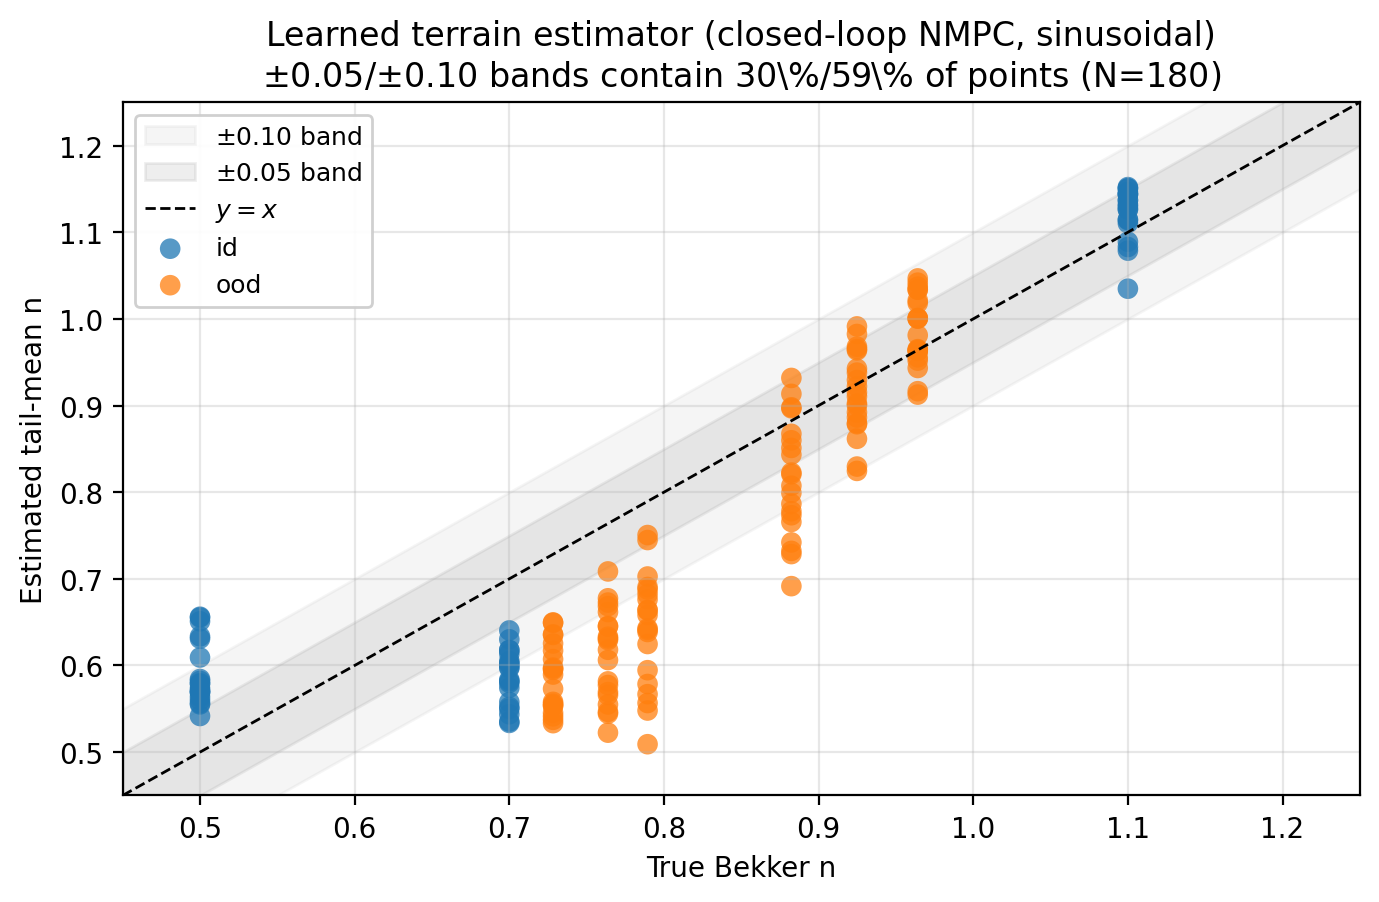
\includegraphics[width=\columnwidth]{terrain_estimator_scatter.png}
  \caption{Learned (sliding-window MLP) terrain estimator: true vs.\
    estimated Bekker $n$ (tail-window mean) on the closed-loop
    sinusoidal benchmark, evaluated \emph{within the estimator's
    training envelope} (bumpiness $\in\{0,4\}$). Blue = in-distribution
    canonical soils (clay/dirt/sand); orange = Bekker-jittered
    out-of-distribution soils ($n$ sampled in $[0.40,1.30]$, other five
    Bekker parameters perturbed $\pm 30\text{--}50\,\%$). The
    $\pm 0.05$ / $\pm 0.10$ bands around $y=x$ contain $40\,\%$ / $68\,\%$
    of points. The estimator tracks the diagonal across the deployment
    range, with a mild systematic over-prediction in the lowest-$n$
    (clay) bin (mean estimate $0.59$ vs.\ true $0.50$). See the
    out-of-envelope note in the text for behaviour at bumpiness $8$.}
  \label{fig:estimator_scatter}
\end{figure}

\begin{figure}[!t]
  \centering
  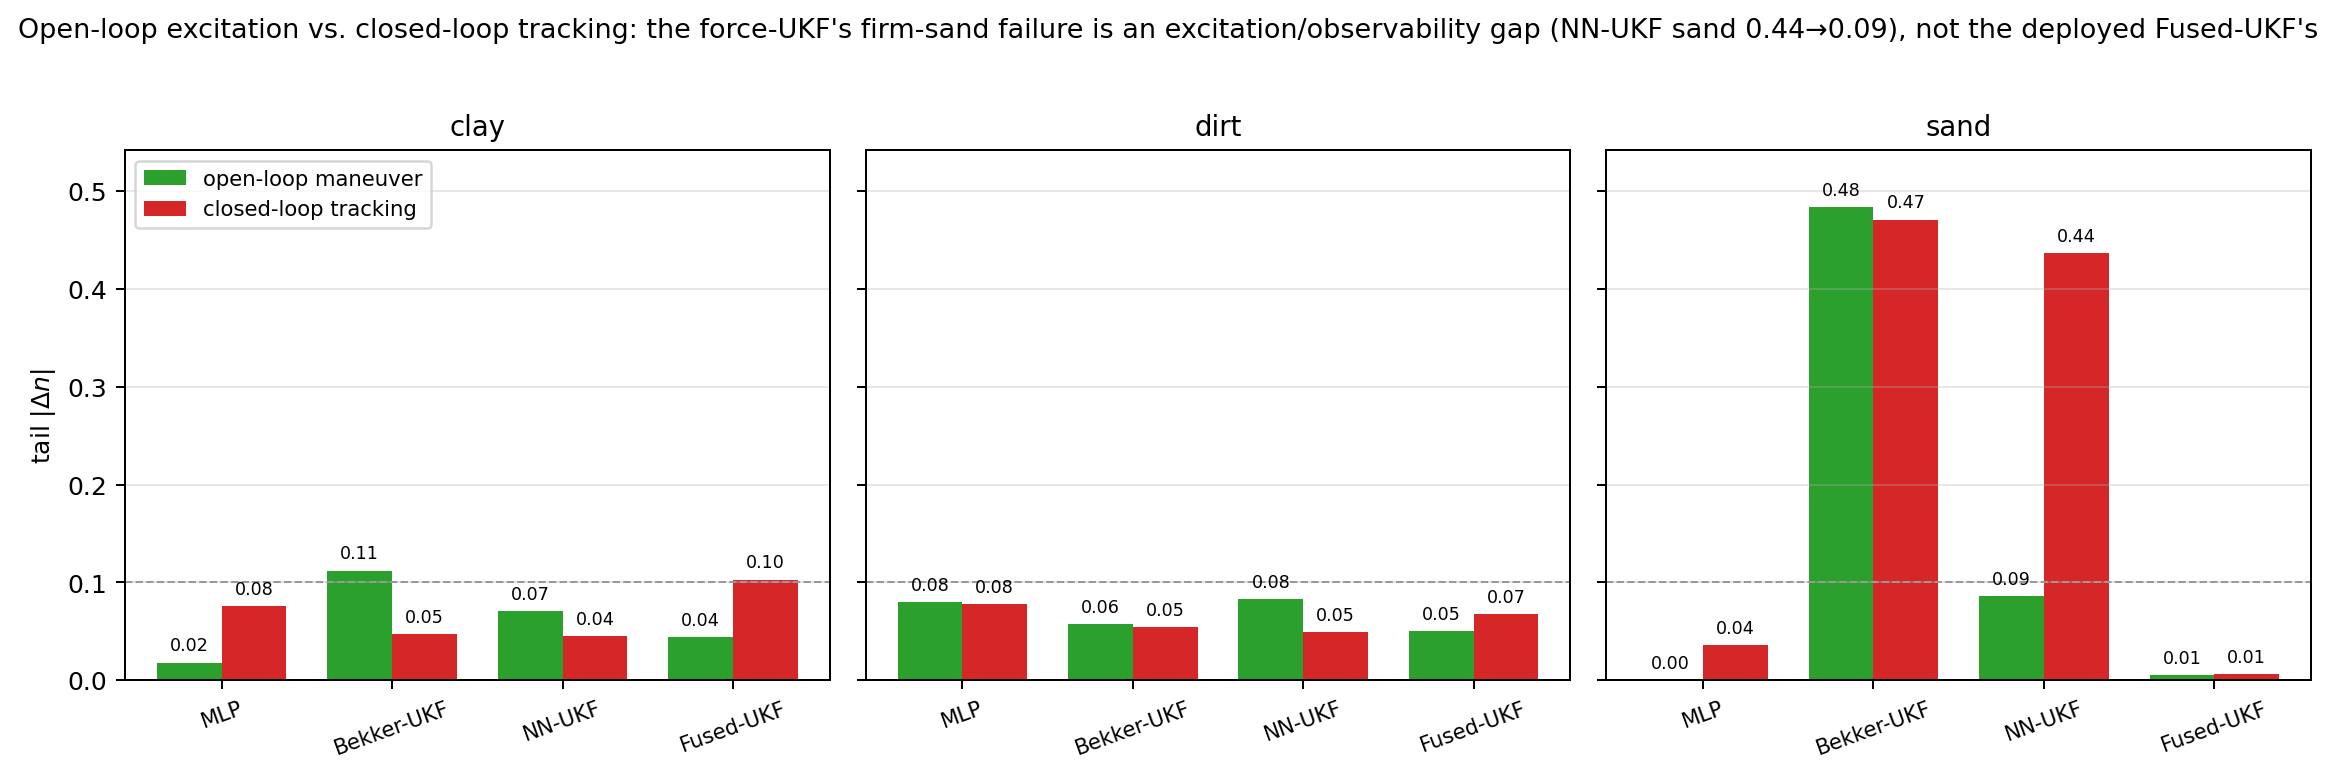
\includegraphics[width=\columnwidth]{open_loop_estimator_diagnostic.png}
  \caption{Open-loop excitation vs.\ closed-loop tracking, all four
    estimators, canonical soils (tail $|\Delta n|$). A scripted
    $0.6\,$rad sine-steer maneuver (green) is compared to closed-loop
    NMPC path-tracking (red). On firm sand the force-only NN-UKF is
    \emph{observability}-limited --- accurate under the scripted maneuver
    ($0.09$) but drifting under closed-loop tracking ($0.44$), so a
    dedicated maneuver resolves it --- whereas the Bekker-UKF remains
    $\approx\!0.47$ in both (\emph{model}-limited: its analytical contact
    law is inaccurate on sand). The proprioceptive MLP is
    excitation-agnostic ($0.00\!\to\!0.04$), and the deployed Fused-UKF is
    accurate in both ($\approx\!0.01$),
    so it needs no dedicated maneuver at runtime
    (cf.\ Sec.~\ref{sec:ukf}).}
  \label{fig:estimator_open_loop}
\end{figure}

\paragraph{Out-of-envelope behaviour (bumpiness).}
The learned estimator's window features include a vertical-dynamics
block ($a_z$ and pitch/roll-rate statistics) that senses how strongly
the chassis rides over terrain undulation; these features were trained
only at bumpiness $\in\{0,4\}$ (Table~\ref{tab:training_data}). At
bumpiness $8$ --- outside that training envelope --- the bump-induced
vertical excitation is mis-read as firm-soil stiffness and the estimate
on soft clay diverges upward: the tail-mean estimate at $n=0.5$ rises
from $0.59$ in-envelope to $1.03$ ($|\Delta n|\!\approx\!0.53$), i.e.\
the estimator reports near-firm soil on the softest terrain. This is a
genuine out-of-distribution failure on the bumpiness axis, not a
low-$n$ failure per se --- clay is estimated accurately
($|\Delta n|\!\approx\!0.09$) at bumpiness $\le 4$. It is a limitation
of the window-MLP channel alone, not of the deployed Fused-UKF: its
state-augmented force channel (Sec.~\ref{sec:ukf}) infers $n$ through a
physics-based bicycle model and does not show this bumpiness sensitivity.
Extending the training set to higher bumpiness, or gating the
vertical-dynamics features on an online road-roughness estimate, would
close the gap and is left to future work; results here are reported
within the trained envelope.

\subsection{Closed-loop terrain estimation: force observability and a proprioceptive-fused UKF}
\label{sec:estimator_ukf}
\label{sec:ukf}

The deployed terrain estimator is a \textbf{Fused-UKF}: a
state-augmented unscented Kalman filter that, following the
state-augmentation idea of Dallas et al.~\cite{Dallas21}, estimates
the Bekker sinkage exponent $n$ jointly with the bicycle state, but
fuses \emph{two} measurement channels of $n$ rather than one.
\textbf{(i)} A whole-vehicle lateral-force channel: a learned surrogate
maps the bicycle's own state plus the six Bekker--Mohr soil parameters
to $(F_{y,\mathrm{total}}, M_{\mathrm{yaw,total}})$, and the UKF
observes the body-frame $a_y$ as a direct measurement of
$\Sigma F_y/m$. \textbf{(ii)} A proprioceptive channel: the deployed
\emph{heteroscedastic} sliding-window MLP supplies an independent
measurement $n_{\mathrm{MLP}}$ \emph{together with} its own per-sample
uncertainty $\sigma_{\mathrm{MLP}}$, which the UKF consumes as the
proprioceptive measurement noise $R_n$. The full measurement vector is
$[x,y,\psi,u,v,\omega,\,a_y,\,n_{\mathrm{MLP}}]^\top$, and the two
$n$-channels are weighted purely by Kalman covariance --- there is
\emph{no} hand-tuned gate or external blend. The MLP is trained with a
Gaussian negative-log-likelihood objective (val RMSE$_n$ $0.064$;
$\mathrm{corr}(|\mathrm{err}|,\sigma_{\mathrm{MLP}})\!=\!0.71$), so it
reports low $\sigma$ exactly where it is accurate --- notably on firm
sand --- and the filter automatically trusts it there.

We compare the deployed Fused-UKF against two force-only baselines that
share the identical UKF and bicycle but drop the proprioceptive
channel: \textbf{(i) Bekker-UKF}, an analytical Bekker--Wong
contact-patch integration that mirrors the SCM plant's own formulation,
and \textbf{(ii) NN-UKF (force-only)}, the whole-vehicle lateral-force
surrogate driving the prediction step with no proprioceptive
measurement. The bicycle is the 4-wheel double-track variant of
Dallas's 3-DOF model --- each wheel receives its own vertical load
under quasi-static longitudinal and lateral transfer driven by measured
$a_x$, $a_y$, the steering input, and the body-frame yaw rate.

\paragraph{Whole-vehicle lateral-force surrogate.} The UKF's force
channel predicts what the \emph{whole vehicle} produces directly, rather
than scaling a single-tire rig force by a hand-tuned rig-to-vehicle gain.
A rig-plus-gain calibration holds at the soft-soil presets but does not
generalise across a broad LHS sweep, so the deployed surrogate is trained
end-to-end on whole-vehicle forces:
\[
  \resizebox{\columnwidth}{!}{$\displaystyle
  \mathrm{NN}_{F_y}\!:\, (u, v, \omega, \delta, K_\phi, K_c, n,
  c, \phi, k)\ \mapsto\ (F_{y,\mathrm{total}},\ M_{\mathrm{yaw,total}})$}.
\]
The surrogate is a 128--64 ReLU MLP trained on a 300-sample,
9-axis uniform LHS sweep
(seed 7)
that varies the six Bekker--Mohr soil parameters together with three
maneuver axes --- steering amplitude $0.20\text{--}0.65\,$rad,
steering period $2\text{--}5\,$s, and target cruise speed
$3.5\text{--}7\,$m/s (half the runs use constant open-loop throttle,
half a PI cruise) --- yielding $\approx 190\,000$ labelled rows.
Crucially, the soil axes are sampled from a \emph{widened} box
($K_\phi$ from $0.3\,$MPa, cohesion from $300\,$Pa, Janosi shear
$0.008\text{--}0.028\,$m, $n\in[0.35,1.35]$): the canonical clay,
dirt and sand presets sit on the \emph{edges} of the deployed
training box (clay's $K_\phi$ is at $5\,\%$ of
range and its Janosi shear at the $0\,\%$ floor), so a surrogate
trained on that box has to extrapolate to reach them and fails on
clay. Widening the box (never narrowing, so the uniform LHS coverage
is preserved) turns those soils into interior points the surrogate
interpolates to.
Targets are extracted directly from each Chrono log:
$F_{y,\mathrm{total}}\!=\!m\,a_y$ and
$M_{\mathrm{yaw,total}}\!=\!I_z\,\dot\omega$ (5-point central
difference). Held-out (30 of 300 scenarios, scenario-split) $R^2$ is
$0.90$ on $F_y$ and $0.88$ on $M_{\mathrm{yaw}}$. Every input axis is
uniformly sampled over the widened box, with no narrowing toward a
canonical preset or controller-conditioned operating point, and the
trained model enters the UKF with no per-soil scalar correction. This
surrogate is the UKF's force channel for both the Fused-UKF and the
force-only NN-UKF.

\paragraph{Force observability of $n$ (the key issue).}
The reason the force channel alone is not enough is an
\emph{observability} gap, not a model defect. Under a path-tracking
controller the slip stays small, and at that operating point the
lateral force carries almost no information about $n$ on firm soil. At
a representative small-slip operating point the lateral-force signal
separating firm from soft soil is
$|F_y(n\!=\!1.1)-F_y(n\!=\!0.7)|\!\approx\!132\,$N, well below the
lateral-accel measurement-noise floor of
$\approx\!770\,$N ($=m\,R_{a_y}$ with $R_{a_y}\!=\!0.3\,$m/s$^2$). Under
a \emph{scripted} $0.6\,$rad steering maneuver the same delta grows to
$743\,$N --- at the noise floor --- and $\mathrm{d}F_y/\mathrm{d}n$ is
$\approx\!16\times$ larger. The yaw channel is worse still:
$|\mathrm{d}M_z|\,\Delta n\!\approx\!191\,$N$\cdot$m sits below its
$\approx\!216\,$N$\cdot$m noise floor and stays unobservable even at
large slip. A force-only UKF is therefore \emph{blind} to firm-soil $n$
under gentle tracking: the signal it would need to correct $n$ is
buried in the measurement noise. Fig.~\ref{fig:ukf_observability}
makes this concrete --- and shows that the proprioceptive channel,
which reads vibration rather than slip-dependent force, fills exactly
this gap.

\begin{figure}[!t]
  \centering
  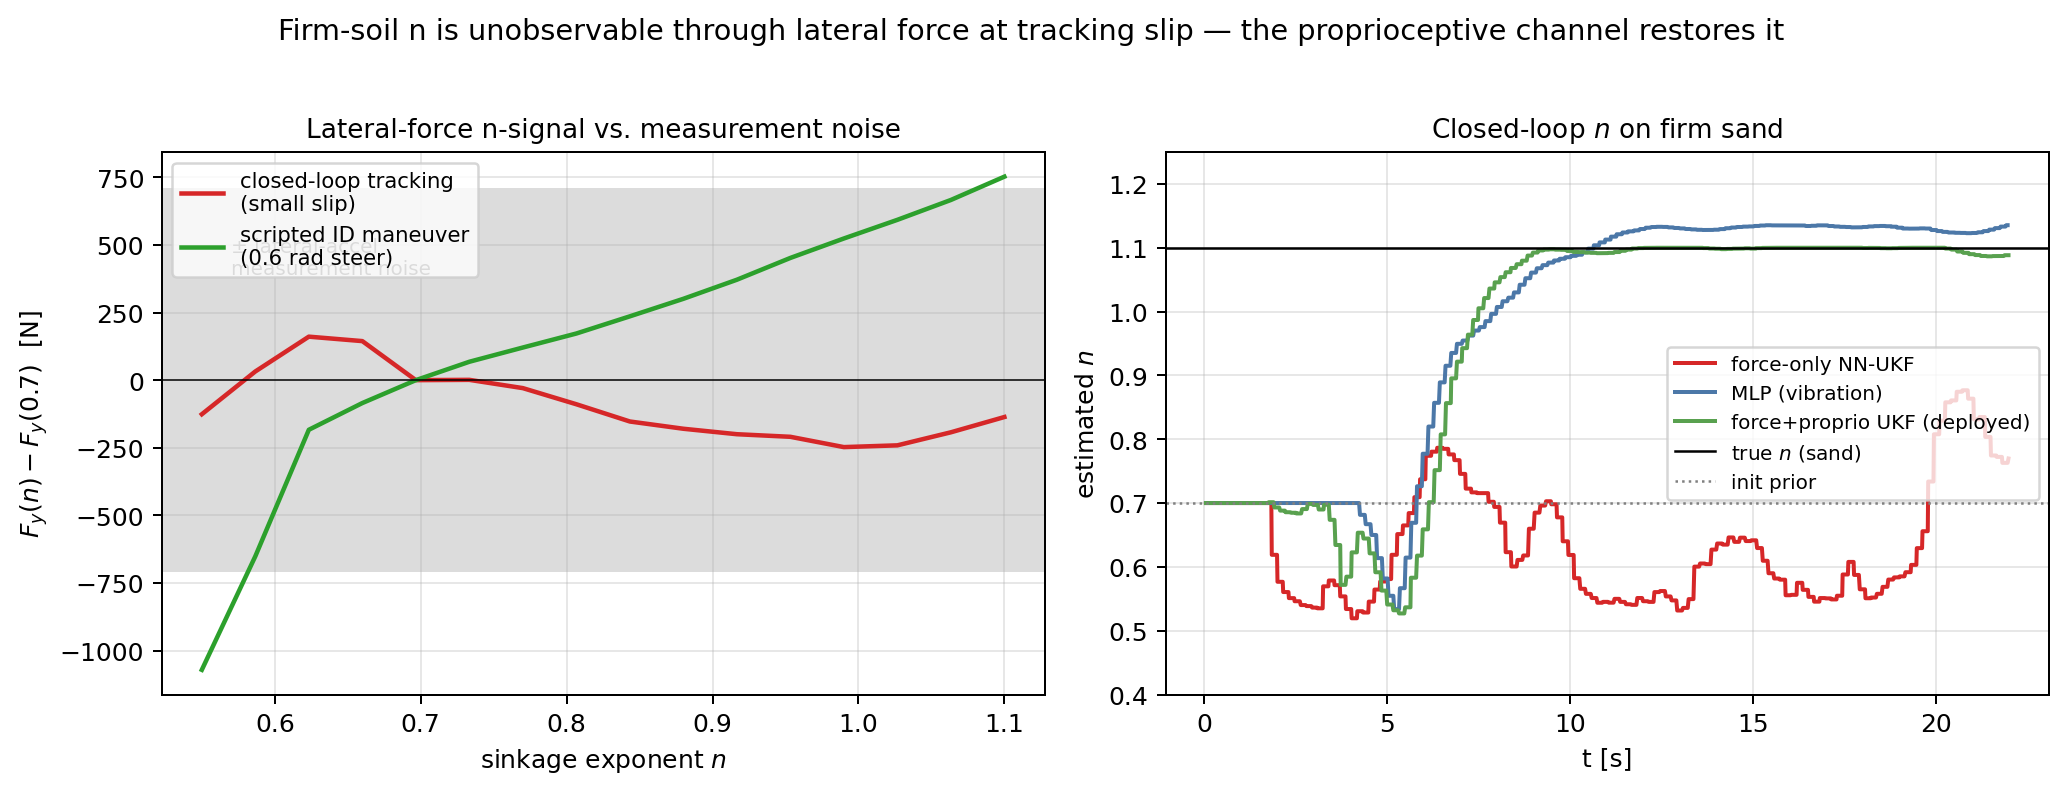
\includegraphics[width=\columnwidth]{ukf_observability.png}
  \caption{Force observability of the sinkage exponent $n$.
    \textbf{Left:} the lateral-force $n$-signal
    $|F_y(n\!=\!1.1)-F_y(n\!=\!0.7)|$ against the lateral-accel
    measurement-noise band ($m\,R_{a_y}\!\approx\!770\,$N,
    $R_{a_y}\!=\!0.3\,$m/s$^2$). At closed-loop small-slip path
    tracking the signal ($\approx\!132\,$N) stays \emph{inside} the
    band --- $n$ is unobservable from force --- whereas a scripted
    $0.6\,$rad maneuver escapes it ($\approx\!743\,$N, with
    $\mathrm{d}F_y/\mathrm{d}n$ $\approx\!16\times$ larger). \textbf{Right:}
    closed-loop $\hat n(t)$ on firm sand: the force-only NN-UKF, lacking
    an observable force signal, drifts in the \emph{wrong} direction, while the
    deployed Fused-UKF tracks the true $n$ by leaning on its
    proprioceptive channel.}
  \label{fig:ukf_observability}
\end{figure}

\paragraph{Open-loop vs.\ closed-loop: two distinct failure modes.}
The earlier open-loop diagnostic (Fig.~\ref{fig:estimator_open_loop})
separates an \emph{observability} limit from a \emph{model} limit by
comparing each estimator's tail $|\Delta n|$ on firm sand under a
scripted excitation maneuver against the same soil under closed-loop
tracking. The force-only NN-UKF goes from $0.09$ (open-loop) to $0.44$
(closed-loop): it is observability-limited, and a dedicated excitation
maneuver \emph{resolves} it. The Bekker-UKF, by contrast, is essentially
unchanged across the two ($0.48\!\to\!0.47$): it is \emph{model}-limited
--- the analytical Bekker law is inaccurate on sand, and no amount of
excitation can compensate. The
proprioceptive MLP, which reads vibration and is excitation-agnostic,
is accurate in both ($0.00\!\to\!0.04$), and the Fused-UKF inherits that
robustness ($0.01\!\to\!0.01$). This is the observability story seen
from the other side, and it is why the deployed estimator needs
\emph{no} dedicated excitation maneuver at runtime.

\paragraph{The deployed Fused-UKF closes the gap (canonical presets).}
Fig.~\ref{fig:estimator_comparison} reports the four estimators run
\emph{live in the closed loop} on the canonical clay/dirt/sand presets
at $v\!\in\!\{5,7\}\,$m/s (three seeds each); all numbers are tail
$|\Delta n|$ (lower is better). The proprioceptive MLP gives clay
$0.076$, dirt $0.078$, sand $0.036$ (overall $0.063$); the Bekker-UKF
$0.047$, $0.054$, $0.471$ (overall $0.190$); the force-only NN-UKF
$0.045$, $0.049$, $0.437$ (overall $0.162$); and the deployed Fused-UKF
$0.103$, $0.068$, $0.006$ (overall $0.059$). The two force-only UKFs
collapse on firm sand ($\approx\!0.44\text{--}0.47$) for exactly the
observability reason above, whereas the proprioceptive channel makes
$n$ observable, so the Fused-UKF accurately recovers firm sand
($|\Delta n|\!=\!0.006$) and is the most accurate estimator overall
($0.059$). The Fused-UKF is \emph{least} accurate on canonical clay
($0.103$), where both force-only UKFs and the MLP outperform it, because
the proprioceptive channel is slightly over-weighted on soft, on-manifold
soil where the force channel is already reliable. The trade is
favourable: a small clay penalty in exchange for eliminating the
firm-sand failure both force-only baselines exhibit.

\begin{figure*}[!t]
  \centering
  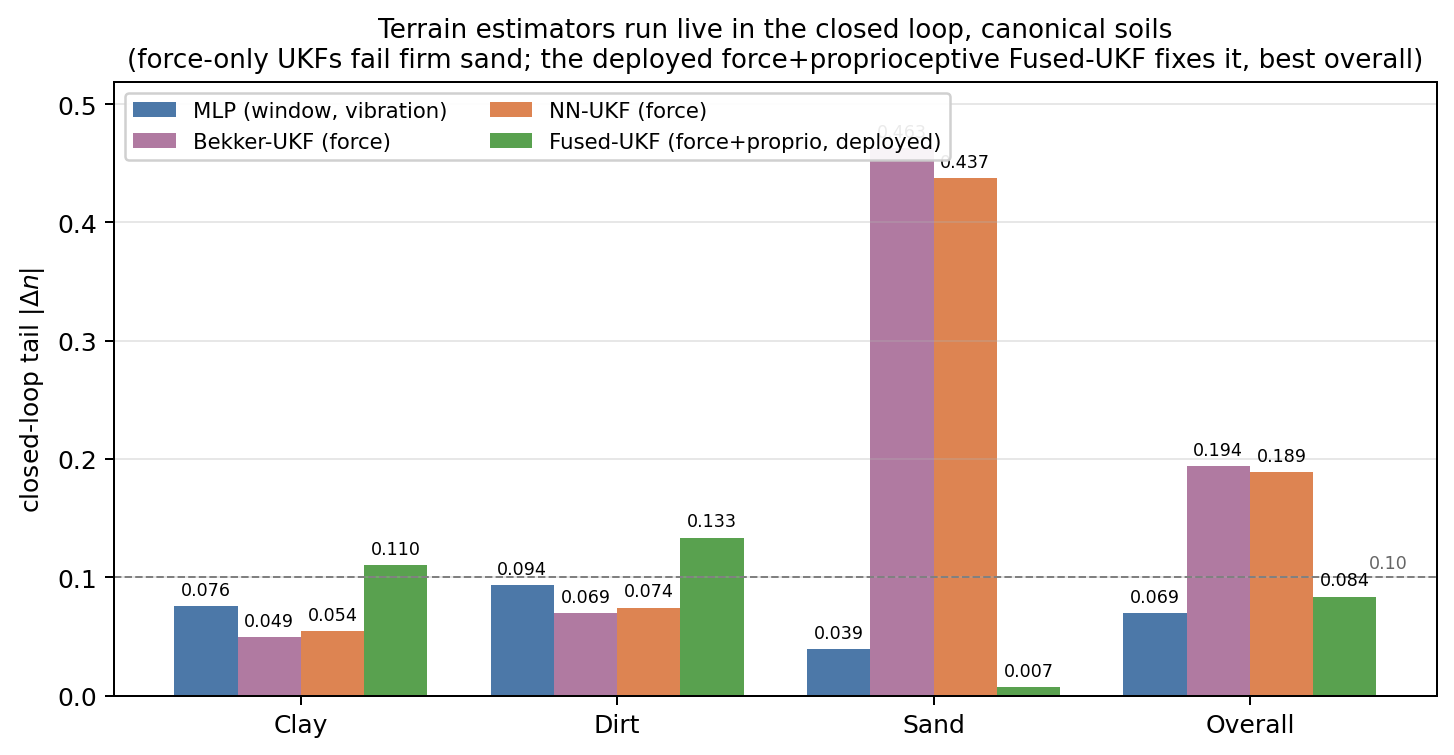
\includegraphics[width=\textwidth]{terrain_estimator_comparison.png}
  \caption{Per-terrain closed-loop comparison of the four estimators on
    the canonical Chrono SCM presets --- clay, sandy loam (dirt), dry
    sand --- run \emph{live} in the loop at $v\!\in\!\{5,7\}\,$m/s,
    three seeds, $0.6\,$rad steering, tail $|\Delta n|$. The Bekker-UKF
    and force-only NN-UKF are most accurate on the soft soils but fail
    on firm sand ($|\Delta n|\!\approx\!0.44\text{--}0.47$, an
    observability limit, cf.\ Fig.~\ref{fig:ukf_observability}); the
    proprioceptive MLP is balanced; the deployed Fused-UKF recovers firm
    sand to $0.006$ at the cost of being least accurate on soft clay
    ($0.103$).}
  \label{fig:estimator_comparison}
\end{figure*}

\begin{figure}[!t]
  \centering
  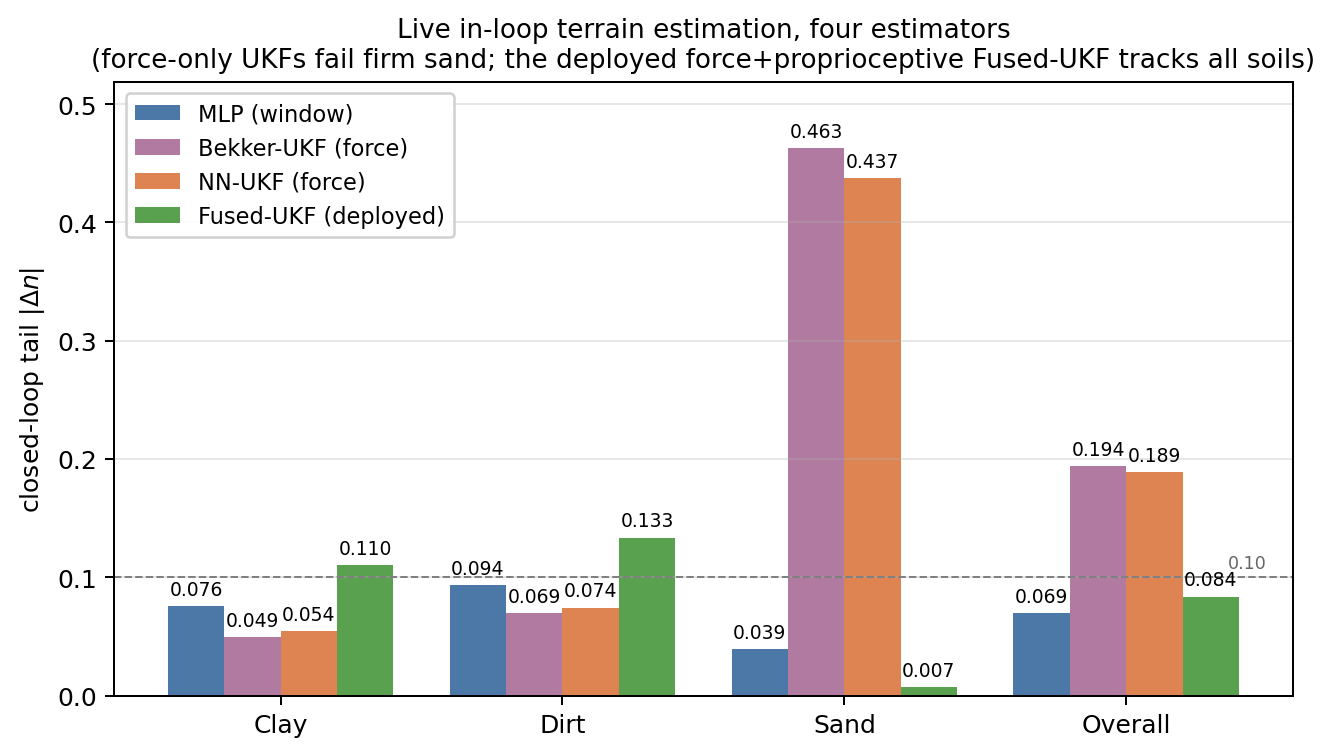
\includegraphics[width=\columnwidth]{closed_loop_estimator_backends.png}
  \caption{Deployment summary: tail $|\Delta n|$ over the canonical
    clay/dirt/sand presets and the overall mean for the proprioceptive
    MLP, the analytical Bekker-UKF, the force-only NN-UKF, and the
    deployed Fused-UKF (all run live in the closed loop,
    $v\!\in\!\{5,7\}\,$m/s, three seeds). The force-only UKFs fail firm
    sand; the covariance-fused proprioceptive channel makes $n$
    observable, so the Fused-UKF is best overall ($0.059$) with no
    hand-tuned gate.}
  \label{fig:cl_estimator_backends}
\end{figure}

\paragraph{Broad robustness across the deployable $n$ range.}
Fig.~\ref{fig:estimator_lhs100} and Table~\ref{tab:estimator_lhs100}
report the head-to-head on \textbf{100 soils swept along the canonical
clay--dirt--sand Bekker--Mohr manifold} (seed 42,
$n\!\in\![0.52,1.08]$; the other five soil parameters follow the preset
manifold with $\pm 8\,\%$ jitter --- the parameter-known setting in
which the force-dominant exponent $n$ is isolated, and the soil model
the estimator reconstructs from $\hat n$), \emph{all} run live
closed-loop under NMPC sinusoidal path-tracking at $5\,$m/s. The
deployed Fused-UKF and the proprioceptive MLP recover $n$ across the
full range (median error $3.8\,\%$ and $7.8\,\%$; $94\,\%$ and
$76\,\%$ within $\pm 20\,\%$), their estimates tracking the diagonal.
The force-only NN-UKF and Bekker-UKF instead saturate near
$n\!\approx\!0.6$ on firm soils ($23.8\,\%$ median error): without a
proprioceptive channel they cannot observe $n$ once closed-loop slip is
small --- the force-observability limit of Sec.~\ref{sec:ukf}, now
visible across the whole sweep rather than only on canonical sand. The
deployed Fused-UKF leads every metric (Fig.~\ref{fig:estimator_overall}), and
the same ranking holds on the canonical clay/dirt/sand presets
(Fig.~\ref{fig:cl_estimator_backends}).

\begin{figure*}[!t]
  \centering
  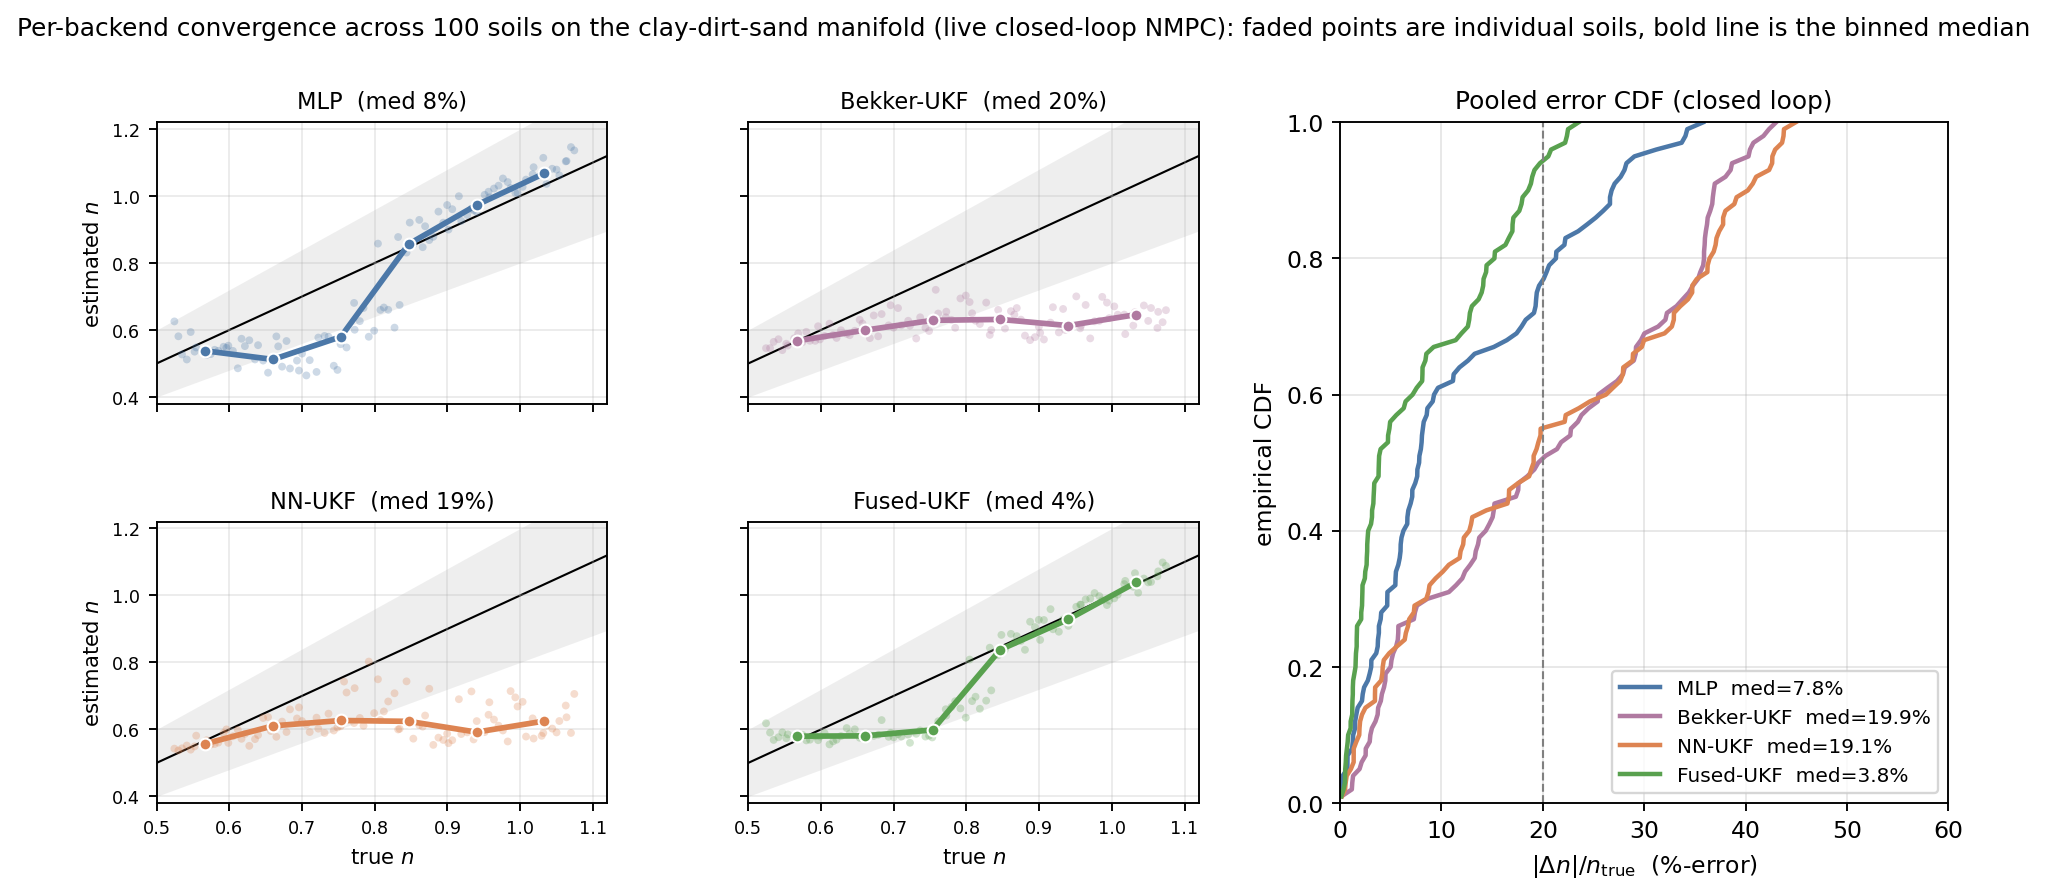
\includegraphics[width=\textwidth]{lhs100_fair.png}
  \caption{Closed-loop terrain-estimator benchmark on 100 soils swept
    along the clay--dirt--sand Bekker--Mohr manifold in Chrono SCM
    (seed 42, $n\!\in\![0.52,1.08]$; the other five soil parameters
    follow the preset manifold with $\pm 8\,\%$ jitter --- the
    parameter-known setting in which the force-dominant exponent $n$ is
    estimated, and the soil model our estimator reconstructs from
    $\hat n$), all run live under closed-loop NMPC sinusoidal
    path-tracking at $5\,$m/s. Left, four panels: estimated $n$ versus
    true $n$ per backend, where faded points are individual soils, the
    bold line is the binned median, and the black diagonal with its
    $\pm 20\,\%$ band is the target. The proprioceptive MLP and the
    deployed Fused-UKF track the diagonal (fitted slope $1.25$ and
    $1.07$), whereas the force-only NN-UKF and Bekker-UKF saturate near
    $n\!\approx\!0.6$ on firm soils (slope $0.15$ and $-0.11$) --- the
    closed-loop force-observability limit quantified in
    Sec.~\ref{sec:ukf}. Right: pooled empirical CDF of the tail-window
    $|\Delta n|/n_{\mathrm{true}}$; the Fused-UKF holds the tightest
    distribution and the best fraction within $\pm 20\,\%$ (dashed
    line).}
  \label{fig:estimator_lhs100}
\end{figure*}

\begin{table}[!t]
  \renewcommand{\arraystretch}{1.10}
  \caption{Closed-loop terrain-estimator head-to-head on 100 soils
    swept along the clay--dirt--sand Bekker--Mohr manifold
    ($n\!\in\![0.52, 1.08]$, seed 42), all run live under closed-loop
    NMPC sinusoidal path-tracking at $5\,$m/s. The other five soil
    parameters follow the preset manifold ($\pm 8\,\%$ jitter), the
    parameter-known setting for isolating the force-dominant exponent
    $n$. Errors are tail-window $|\Delta n|$ (absolute) and
    $|\Delta n|/n_{\mathrm{true}}$ (relative). The deployed Fused-UKF
    row is bold.}
  \label{tab:estimator_lhs100}
  \centering
  \begin{tabular}{lccc}
    \toprule
    \textbf{Estimator} & median $|\Delta n|$ & median \%err
        & within $\pm20\,\%$\\
    \midrule
    MLP        & $0.060$ & $7.8\,\%$  & $76\,\%$\\
    Bekker-UKF & $0.154$ & $19.9\,\%$ & $50\,\%$\\
    NN-UKF     & $0.146$ & $19.1\,\%$ & $55\,\%$\\
    \textbf{Fused-UKF} & $\mathbf{0.033}$ & $\mathbf{3.8\,\%}$
        & $\mathbf{94\,\%}$\\
    \bottomrule
  \end{tabular}
\end{table}

\begin{figure*}[!t]
  \centering
  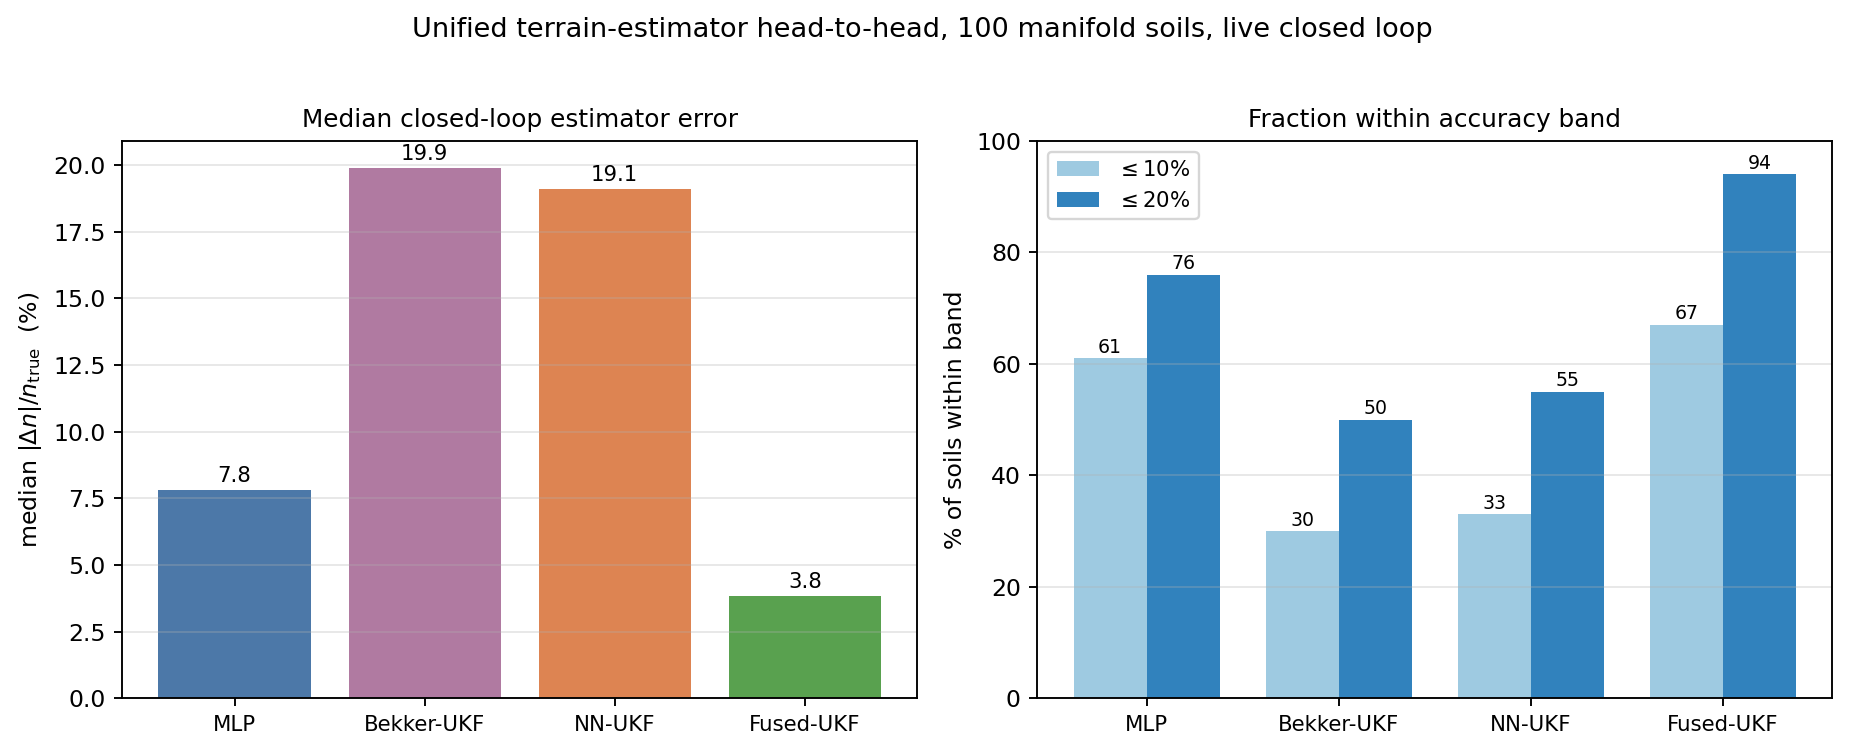
\includegraphics[width=\textwidth]{estimator_overall.png}
  \caption{Pooled closed-loop terrain-estimator comparison over the 100
    manifold soils. \textbf{Left:} median $|\Delta n|/n_{\mathrm{true}}$.
    \textbf{Right:} fraction within the $\pm 10\,\%$ / $\pm 20\,\%$
    bands. The deployed Fused-UKF is the most accurate ($94\,\%$ within
    $\pm 20\,\%$) and the MLP second ($76\,\%$); the force-only NN-UKF
    and Bekker-UKF trail because they cannot observe $n$ on firm soils
    in closed loop, with no hand-tuned gate needed in the Fused-UKF.}
  \label{fig:estimator_overall}
\end{figure*}

%======================================================================
\section{Terrain-Aware Speed Planning}
\label{sec:speedplan}
%======================================================================

The reference-tracking NMPC follows a speed reference $v_{\mathrm{ref}}(s)$
along the path. A purely geometric curvature-limited profile
($v_{\mathrm{ref}}=\sqrt{a_{y,\max}/|\kappa(s)|}$ at a fixed $a_{y,\max}$)
is blind to the soil: on soft terrain it commands cornering speeds the
available grip cannot support, so the vehicle understeers off the line.
The failure is most visible on the high-speed sinusoid, exactly where the
analytical baselines of Sec.~\ref{sec:tires_static} pile up
(Fig.~\ref{fig:tires_static_heatmap}).

We replace it with a terrain-aware, quasi-steady-state time-optimal
profile over a friction-circle (g--g) budget. At each control step the
deployed tire surrogate is queried at the live estimate $\hat n$ and the
per-axle vertical load for the available lateral force
($\!\to a_{y,\max}$) and tractive/braking force
($\!\to a_{x,\max},\,a_{x,\mathrm{brake}}$); a forward--backward pass then
returns the fastest $v_{\mathrm{ref}}(s)$ that keeps the combined demand
inside the circle,
\begin{equation}
  \Big(\tfrac{a_x}{a_{x,\max}}\Big)^{2}
  + \Big(\tfrac{v^{2}\,\kappa(s)}{a_{y,\max}}\Big)^{2} \le 1,
\end{equation}
with a grip-safety margin that de-rates the surrogate's peak-force query
to leave transient headroom. The curvature $\kappa(s)$ is read from the
analytic arc-length spline of the path rather than finite-differenced
over the horizon, whose node spacing varies with speed and otherwise
produces spurious $\kappa$ spikes that collapse $v_{\mathrm{ref}}$.

A closed-loop A/B against the geometric reference (clay/dirt/sand
$\times$ \{sinusoid, double lane change\} $\times\,\{5,7\}\,\mathrm{m/s}$,
five seeds; Fig.~\ref{fig:speedplan}) cuts mean RMS CTE by $36\,\%$
($0.136\!\to\!0.087\,\mathrm{m}$) for a $7\,\%$ reduction in mean speed,
and collapses the across-scenario spread (std $0.17\!\to\!0.06\,\mathrm{m}$).
Here RMS CTE is read as a \emph{controllability} outcome --- whether the
vehicle can hold the planned line under the available grip, rather than a
path-tracking accuracy target --- since a profile that ignores the soil
commands cornering speeds that slide the vehicle off the line.
The gain concentrates on exactly the cells where the curvature heuristic
commands cornering speeds the soil cannot support --- the high-speed
sinusoid on soft soil, where CTE falls by $58$--$71\,\%$ (dirt
$0.618\!\to\!0.260$, clay $0.304\!\to\!0.090\,\mathrm{m}$) --- and is
neutral on the already-benign cells. The trade-off is grip-limited rather
than tunable: raising the safety margin to recover the lost speed yields
little additional speed (on dirt at $7\,\mathrm{m/s}$,
$+0.3\,\mathrm{m/s}$) while tripling CTE ($0.10\!\to\!0.28\,\mathrm{m}$),
so the chosen operating point is near the best achievable speed/accuracy
trade-off. Because the profile reads its grip limits
from whichever tire model the controller carries, the tire-model
comparison of Sec.~\ref{sec:tires_static} holds it fixed at the geometric
reference to isolate the tracking model; the system-level closed-loop
sweeps elsewhere in the paper run the deployed g--g profile.

\begin{figure*}[!t]
  \centering
  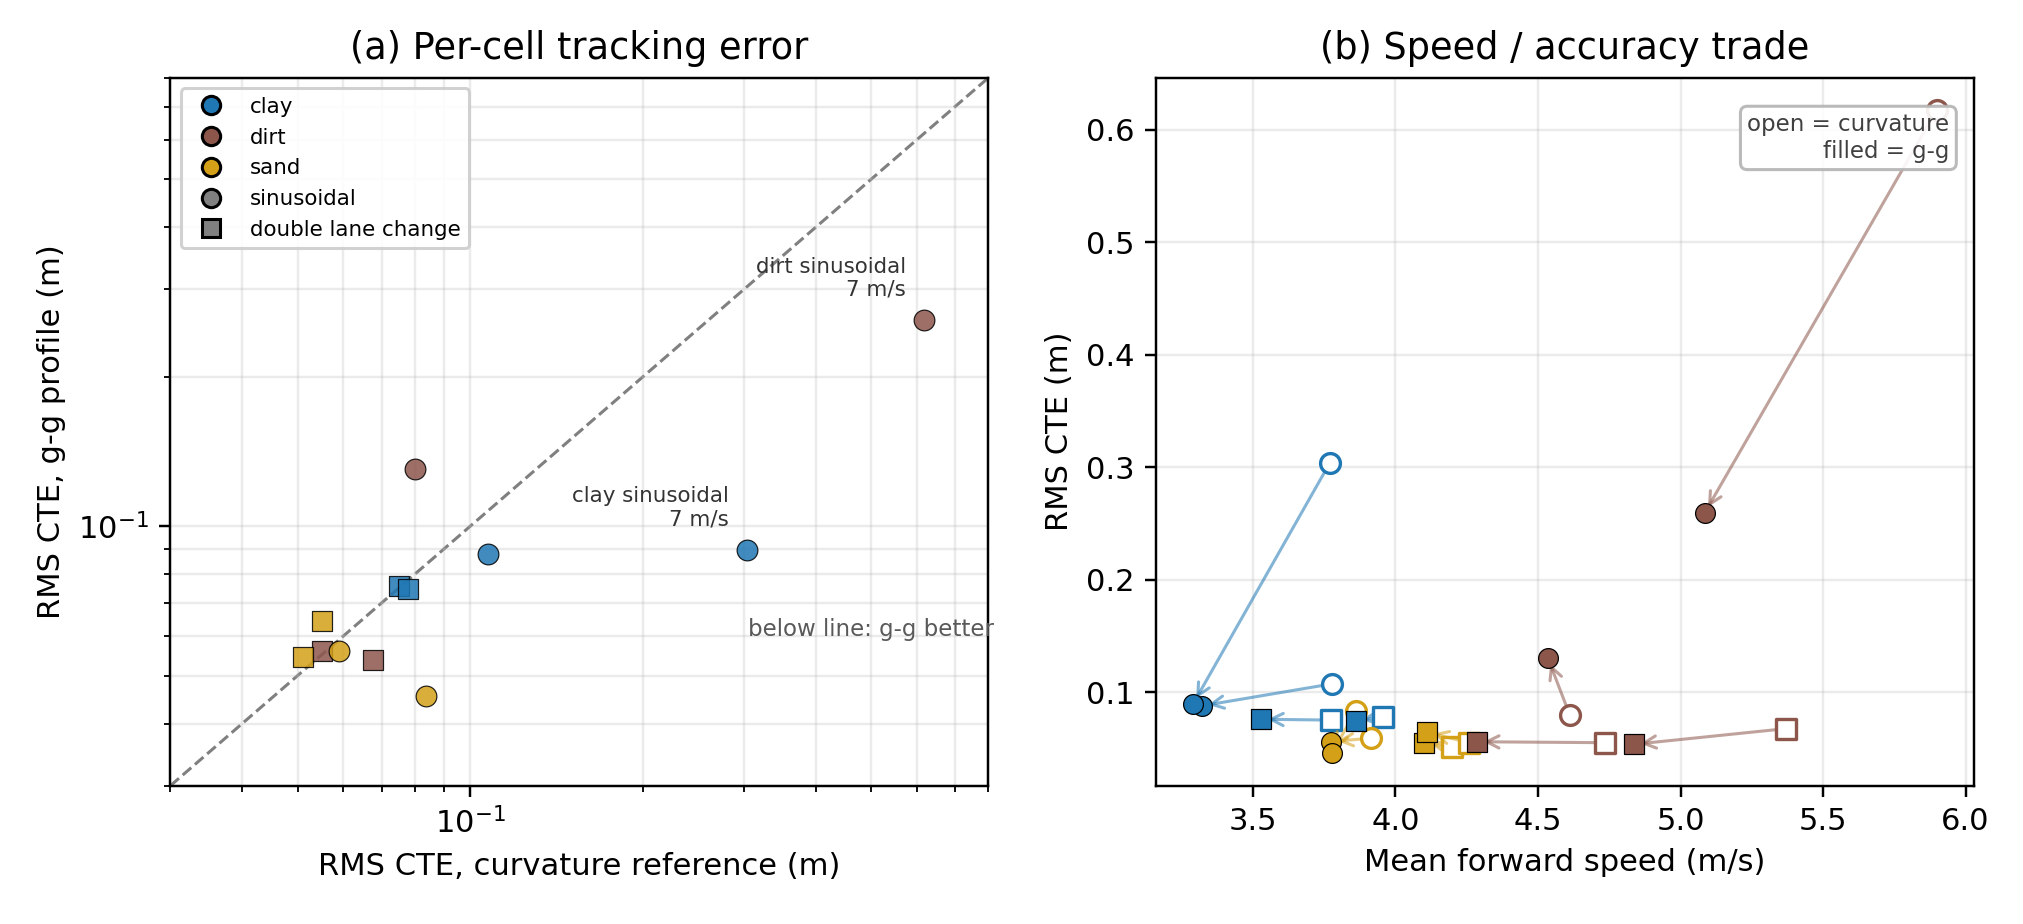
\includegraphics[width=\textwidth]{speed_profile_gg.png}
  \caption{Terrain-aware g--g speed profile vs.\ the geometric
    curvature reference, closed loop. \textbf{(a)} Per-cell RMS CTE: the
    two soft-soil high-speed cells (far right) drop to the trackable
    cluster, while benign cells are unchanged (a few sand cells sit
    marginally above the diagonal, the profile being slightly
    conservative there). \textbf{(b)} Speed/accuracy trade: open markers
    are the curvature reference, filled the g--g profile; arrows show
    each cell trading a little mean speed for a large CTE reduction. The
    grip limits come live from the tire surrogate at $\hat n$
    (Sec.~\ref{sec:tires}).}
  \label{fig:speedplan}
\end{figure*}

%======================================================================
\section{Asymmetric Throttle Disturbance Observer}
\label{sec:throttledob}
%======================================================================

The bicycle-model NMPC integrates the longitudinal velocity $u$
under the open-loop dynamics $\dot u\!=\!a_x$, with $a_x$ the
commanded longitudinal acceleration. On deformable soil the realised
acceleration is consistently smaller than commanded because of
sinkage drag, producing a steady-state under-speed bias. A
first-order integral disturbance observer on the actuation map
absorbs this bias:
\begin{equation}
  \dot d = \begin{cases}
    K_i (u_{\mathrm{ref}} - u), & u < u_{\mathrm{ref}},\\
    -K_b\, d,                   & u \ge u_{\mathrm{ref}},
  \end{cases}
  \quad |d| \le d_{\max},
\end{equation}
with the bleed gain $K_b\!<\!K_i$ to make the observer asymmetric: it
accumulates rapidly during under-speed and decays slowly toward zero,
never contributing a positive over-speed bias. The applied throttle
is $\tau\!=\!\tau_{\mathrm{NMPC}}\!+\!d$. The ablation zeros both
gains ($K_i\!=\!0$, $d_{\max}\!=\!0$), keeping the structural hook
but suppressing all integral action so the comparison is
apples-to-apples. Table~\ref{tab:throttledob} and
Fig.~\ref{fig:throttledob} report the result over 405 closed-loop
runs per variant.

\begin{table}[!t]
  \renewcommand{\arraystretch}{1.15}
  \caption{Asymmetric throttle disturbance observer ablation.
    405 runs per variant. Speed ratio is reported against the
    \emph{terrain-aware g-g speed profile} (Sec.~\ref{sec:speedplan};
    mean $u_\mathrm{meas}/\mathrm{mean}\,v_\mathrm{ref}(s)$) rather than the
    CLI cruise target, because on curvature-heavy paths the profile
    itself caps below the cruise target -- the cruise target is the
    \emph{intent}, the profile is what the controller is
    asked to track. The observer increases achieved speed by approximately
    $5\,\%$ at a small ($\sim$2\,mm) increase in mean tracking error.}
  \label{tab:throttledob}
  \centering
  \setlength{\tabcolsep}{4pt}
  \begin{tabular}{lccc}
    \toprule
    \textbf{Variant} & \textbf{RMS CTE (m)} & \textbf{Speed/profile} & \textbf{$\bar u$ (m/s)}\\
    \midrule
    DOB off & $0.085 \pm 0.034$ & $0.61$ & $4.06$\\
    DOB on  & $0.087 \pm 0.040$ & $\mathbf{0.64}$ & $\mathbf{4.26}$\\
    \bottomrule
  \end{tabular}
\end{table}

\begin{figure*}[!t]
  \centering
  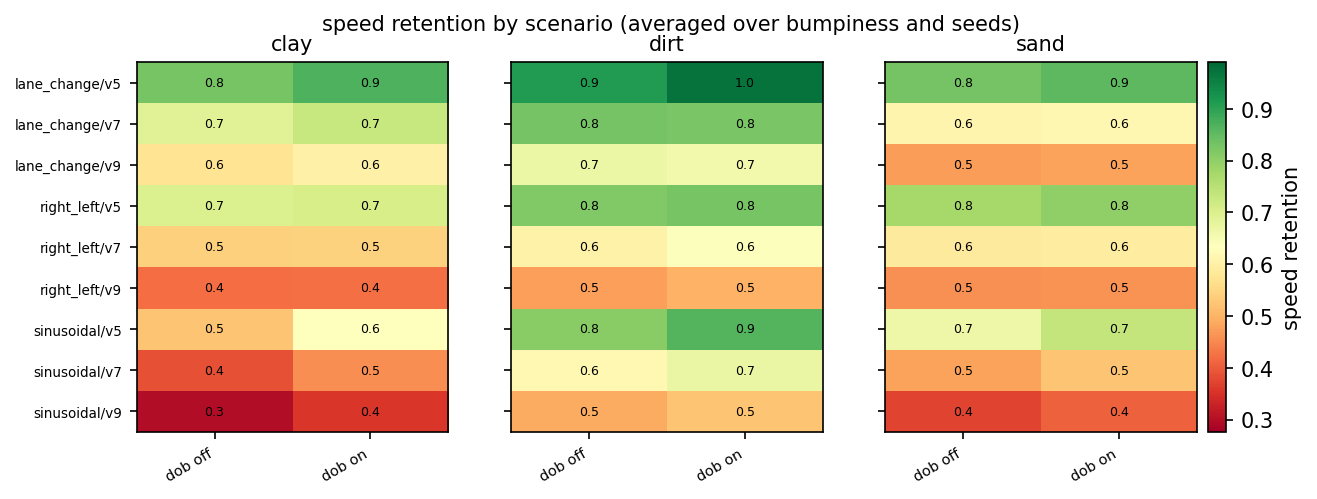
\includegraphics[width=\textwidth]{throttle_dob_ablation_speed_heatmap.png}
  \caption{Throttle disturbance observer ablation: per-scenario
    speed retention (achieved $\bar u$ divided by reference
    $v_{\mathrm{ref}}$) heatmap; row labels show $v_{\mathrm{ref}}$
    and the achieved $\bar u$ so the gap between target and realised
    speed is explicit. The observer's gain is largest on sand at
    $v_{\mathrm{ref}}=7\,\mathrm{m/s}$, consistent with the higher
    sinkage drag in that regime.}
  \label{fig:throttledob}
\end{figure*}

\subsection{Why a reactive observer, not a feedforward model}
\label{sec:throttledob_ff}
A feedforward alternative sets a calibrated longitudinal residual
$\mathrm{d}u_\mathrm{resid} = -c_\mathrm{drag}(\hat n)$ from the DOB-off
drift. It cannot replace the observer, because the prediction bias is not
a monotonic drag but a \emph{sign-varying, terrain-dependent} effect:
firm sand over-predicts speed
($c_\mathrm{drag}\!\approx\!0.17\,\mathrm{m/s^2}$), dirt under-predicts,
and clay is accurate --- and clay's deficit is a traction limit, not a
drag, which only integral feedback closes. Across clay/dirt/sand the DOB
beats the calibrated feedforward on speed ratio at every terrain (clay
$0.70$ vs.\ $0.54$, dirt $0.88$ vs.\ $0.85$, sand $0.67$ vs.\ $0.64$);
baking the converged offset in as a static bias likewise recovers part of
the clay deficit but over-throttles dirt and inflates tracking error,
since the required offset varies with instantaneous speed, curvature, and
load transfer. The disturbance-rejection burden is genuinely adaptive, so
the DOB is the default and a feedforward term is at most an optional
firm-soil refinement.

%======================================================================
\section{Two-Layer Obstacle Avoidance}
\label{sec:safety}
%======================================================================

The planner adds a smooth softplus barrier to the stage and terminal
costs for each known obstacle. Downstream of the planner and human
command source, the safety-filter registry exposes a common filter
interface: the filter receives the desired steering, throttle, brake, the
current state, and the nearby obstacles, and returns the filtered command
plus diagnostics. The
DOB-CBF variant solves a single-step minimum-deviation QP around the
incoming command --- a minimally-invasive control-barrier-function
filter~\cite{Ames19} in the shared-control tradition of predictive and
shared-autonomy teleoperation~\cite{Hirche12,Dragan13}, here with a
disturbance-observer traction budget and physical rate limits; it is the
natural intent-preserving mechanism for HIL teleoperation --- and logs
intervention rate and command deviation as an intrusiveness signal. It also carries a rear-approach guard: when an
in-lane vehicle is closing from behind within a threat distance, it refuses
any deceleration and, with the path ahead clear, accelerates to escape (even
from a standstill), since slowing into a rear approach only worsens the impact
(scope and limits in Sec.~\ref{sec:limitations}). The DOB-CBF output
is passed through a steering/throttle actuator model --- a physical
rate limit imposed in the QP and enforced at the physics step --- so
the filter never commands a non-physical instantaneous reversal that
would otherwise destabilise the front end under teleoperation.

\paragraph{Comparison.}
The safety layer is evaluated as DOB-CBF (the intent-preserving filter
of Zhang et al.~\cite{Zhang25}, optionally reading the same neural
surrogate) versus no filter. The registry remains swappable, but
DOB-CBF is the default instance: it is the only candidate that screens
a human command by minimum deviation rather than re-optimising it, which
is what teleoperation requires.

\subsection{Human-in-the-loop safety-filter protocol}
\label{sec:safety_hil}

The safety filter screens a \emph{human operator's} delayed commands, so
the framework includes a human-in-the-loop (HIL) protocol alongside the
autonomous sweeps below. An operator drives the HMMWV over the
deformable terrain and obstacle field from the Chrono::Sensor camera view
with a Logitech G29 wheel, while the sim-side filter screens each command
immediately before actuation. Every round delays \emph{both} channels:
the command uplink by
$\Delta_\mathrm{cmd} \in \{0, 0.15, 0.30\}\,\mathrm{s}$ and the camera
downlink by $\Delta_\mathrm{cam} = s\,\Delta_\mathrm{cmd}$ ($s=1.0$ for a
symmetric link); a profile-driven delay supplies the learned 5G traces.

The HIL layer reuses the same command contract, swappable safety filters,
latency injection, and metric pipeline as the autonomous evaluation, logging
the same safety and intrusiveness signals (collisions, minimum clearance,
intervention rate, mean steering and throttle/brake correction, speed
retention). Fig.~\ref{fig:hil_hud} shows the operator's view: the
Chrono::Sensor driver point-of-view over the deformable terrain and boulder
field, with the live heads-up display overlaying the delayed command and the
filtered command actually sent to the vehicle.

\paragraph{Scope.}
The HIL pipeline shows the framework can drive a real operator end-to-end
--- G29 input, Chrono::Sensor camera POV, live HUD, and per-channel
latency, all through the same contract and filter as the autonomous stack
(Fig.~\ref{fig:hil_hud}). The \emph{quantitative} safety results come not
from human rounds --- which carry inter-operator variance --- but from the
deterministic \emph{counterfactual} of Sec.~\ref{sec:safety_convoy}: a
fixed command trace replayed filter-off versus DOB-CBF-on over the
\emph{identical} scenario, giving a paired, reproducible
collision-prevention measurement. The traces are worst-case
``drive-into-the-hazard'' commands; since the simulator is deterministic,
the same machinery replays recorded G29 traces unchanged.

\begin{figure}[!t]
  \centering
  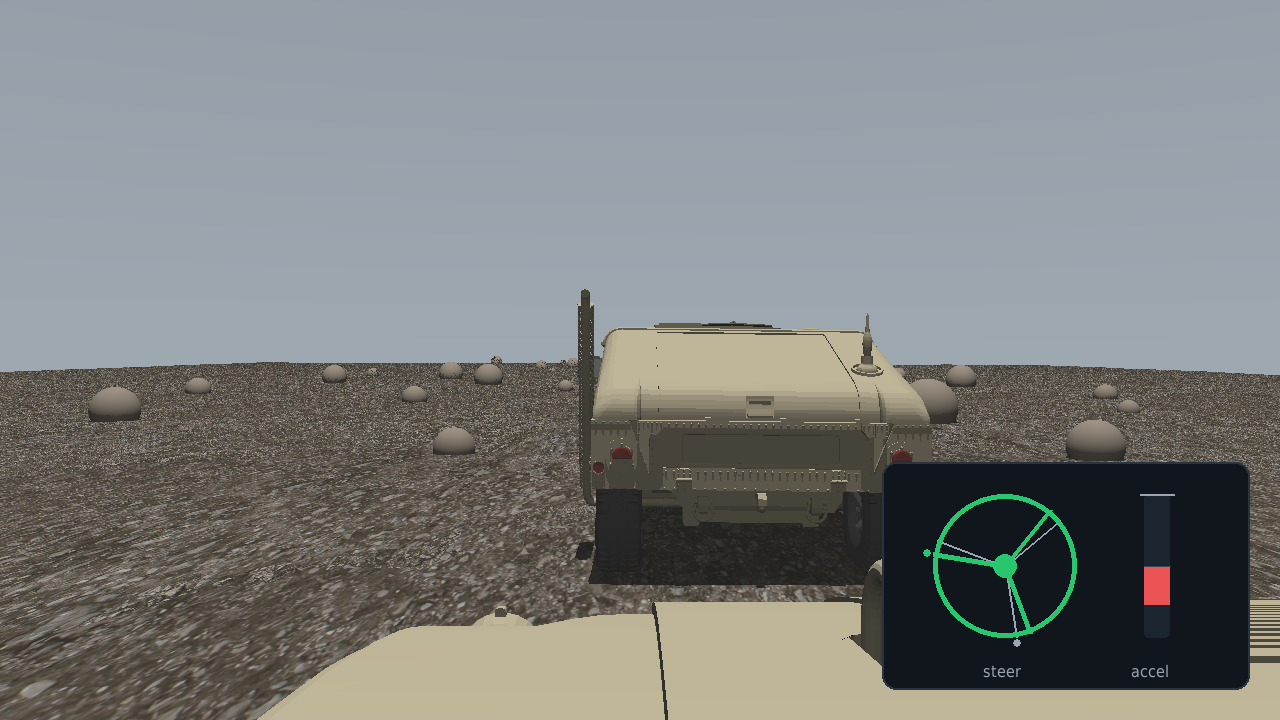
\includegraphics[width=\columnwidth]{hil_hud_pov.png}
  \caption{The human-in-the-loop operator view: the Chrono::Sensor driver
    point-of-view over the SCM deformable terrain and boulder field (the same
    camera feed that carries the downlink latency), with the live HUD
    (\texttt{hil\_hud.py}) overlaying the steering and throttle/brake state ---
    the ghost mark is the delayed operator command, the solid mark the filtered
    command sent to the vehicle. The pipeline is a demonstrated capability;
    the quantitative safety result is obtained from the deterministic
    counterfactual of Sec.~\ref{sec:safety_convoy}, not from human rounds.}
  \label{fig:hil_hud}
\end{figure}


\subsection{Autonomous validation: safety-filter-only collision avoidance}
\label{sec:safety_blind}

The HIL protocol of Section~\ref{sec:safety_hil} is complemented by
an autonomous controlled experiment in which an obstacle-blind planner
stands in for the operator, isolating the safety filter as the sole collision
avoider. This
removes operator variance and supports a larger, fully repeatable
matrix (405 trials per filter; 1215 trials total across three filters).
The same matrix is re-evaluated with the planner's in-horizon barriers
re-enabled in Sec.~\ref{sec:safety_aware}.
Table~\ref{tab:safety_blind} and Fig.~\ref{fig:safety_blind} report the
safety-filter-only outcome. Because the planner is deliberately routed through the obstacles,
crosstrack error is not reported (it would conflate avoidance with poor
tracking); intrusiveness is measured directly, by intervention rate and
the mean absolute steering/throttle correction ($|\Delta\mathrm{steer}|$,
$|\Delta\mathrm{thr}|$) --- the intent-preservation cost a teleoperator
feels. We compare the deployed DOB-CBF against no
filter and a textbook minimum-deviation \emph{vanilla CBF-QP} baseline --- the
same barrier and QP, but without the disturbance observer, the neural traction
surrogate, or the reactive-steering layer. Both filters cut collisions sharply
from the no-filter baseline (DOB-CBF $77\,\%$, $3.04\!\to\!0.71$; vanilla
CBF-QP $87\,\%$, $3.04\!\to\!0.39$), but in opposite ways. The traction-blind
vanilla filter \emph{steers} aggressively around obstacles
($|\Delta\delta|\!=\!0.34$) and clears marginally more of them, but at a
smaller clearance margin ($+0.22\,$m) and by overriding the operator's steering
hard. DOB-CBF's terrain-aware traction budget instead caps the lateral force it
will command, so on low-traction terrain it \emph{brakes} rather than
commanding a swerve the soil may not sustain ($|\Delta\delta|\!=\!0.28$,
$|\Delta\tau|\!=\!0.38$); this keeps a larger clearance margin ($+0.40\,$m) and
preserves steering intent, but occasionally over-brakes a head-on approach into
a low-speed contact (its residual collisions occur at $\sim\!1.9\,$m/s and
concentrate on the softest terrain, clay). This is the expected behaviour of an
intent-preserving \emph{last-resort} filter: as the \emph{sole} geometric
avoider under a deliberately obstacle-blind planner it is out of its design
envelope, which is exactly why the deployed system pairs it with the
planner-aware barrier (Sec.~\ref{sec:safety_aware}), where the two-layer stack
reaches $0.12$ collisions/run.

\begin{table}[!t]
  \renewcommand{\arraystretch}{1.10}
  \caption{Autonomous safety-filter-only validation (planner blind to
    obstacles). 405 runs per filter (1215 total); same scenario matrix
    as Table~\ref{tab:safety_aware}, blind rows only. A textbook vanilla
    CBF-QP and the deployed DOB-CBF both cut collisions sharply; the
    traction-blind vanilla filter avoids marginally more by aggressive
    steering, whereas DOB-CBF keeps a larger clearance margin and overrides
    steering less (its intent-preservation trade-off, see text). Best per
    column in bold. Collisions and clearance are mean$\pm$std over the 405
    runs/filter; $|\Delta\delta|$, $|\Delta\tau|$ are the mean absolute
    steering and throttle command corrections the filter applies.}
  \label{tab:safety_blind}
  \centering
  \setlength{\tabcolsep}{3pt}
  \footnotesize
  \begin{tabular}{lccccc}
    \toprule
    \textbf{Filter} & \textbf{Coll./run} & \textbf{Clearance (m)} & \textbf{Interv. (\%)} & $\mathbf{|\Delta\delta|}$ & $\mathbf{|\Delta\tau|}$\\
    \midrule
    None             & $3.04\!\pm\!1.17$ & $-1.83\!\pm\!0.32$ & --- & --- & ---\\
    Vanilla CBF-QP   & $\mathbf{0.39\!\pm\!0.59}$ & $+0.22\!\pm\!1.33$ & $50$ & $0.34$ & $\mathbf{0.25}$\\
    \textbf{DOB-CBF} & $0.71\!\pm\!0.78$ & $\mathbf{+0.40\!\pm\!1.94}$ & $58$ & $\mathbf{0.28}$ & $0.38$\\
    \bottomrule
  \end{tabular}
\end{table}

\begin{figure*}[!t]
  \centering
  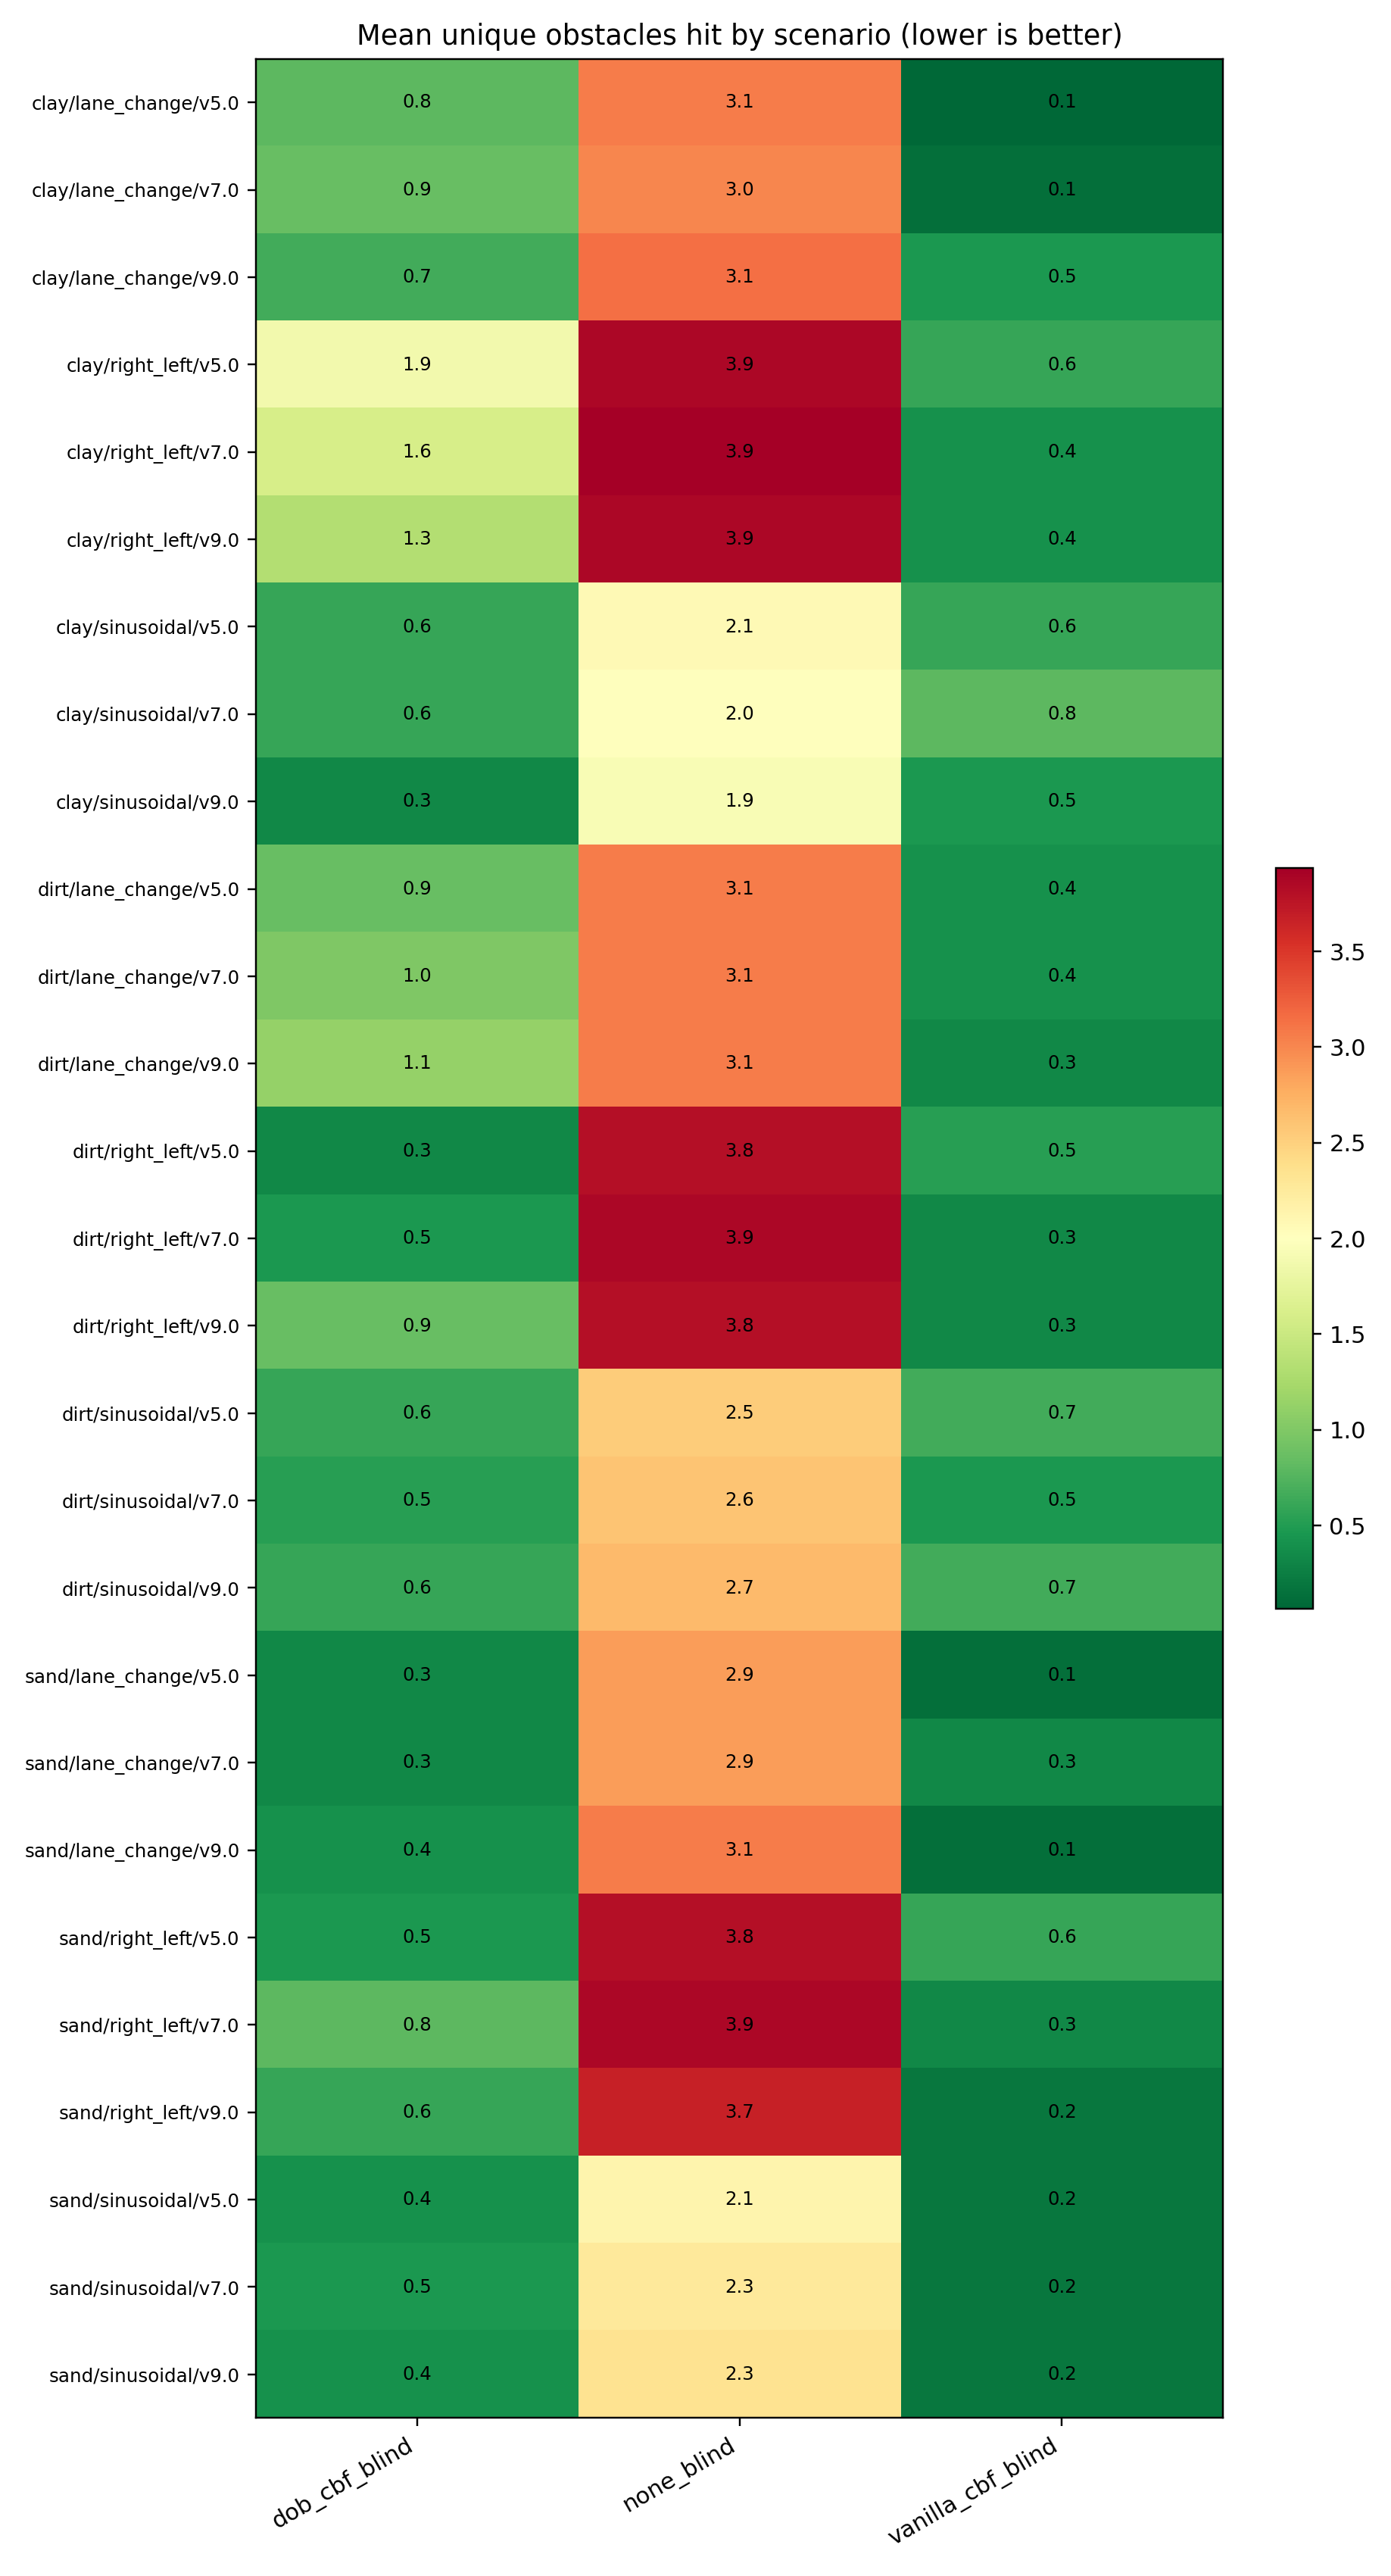
\includegraphics[width=\textwidth]{safety_filter_collision_heatmap.png}
  \caption{Autonomous safety-filter-only validation. Mean unique obstacles hit
    per run, stratified by terrain and safety filter, with whisker
    error bars showing across-seed standard deviation. The reported
    sweep covers all three deployment terrains (clay, dirt, sand) across
    three speeds and three bumpiness levels, $135$ runs per (filter,
    terrain) cell. Aggregate KPIs are in
    Table~\ref{tab:safety_blind}.}
  \label{fig:safety_blind}
\end{figure*}

\subsection{Two-layer (planner-aware) stack}
\label{sec:safety_aware}

With the in-horizon NMPC barrier re-enabled the two-layer stack is
evaluated. Table~\ref{tab:safety_aware} reports 1620 runs total
across the two safety-filter variants (none, DOB-CBF) under both
planner-aware and planner-blind modes.
The honest attribution is two-layer: the in-horizon barrier alone
(no-filter, planner-aware) does the bulk of the work, cutting collisions
roughly $5\times$ relative to the planner-blind baseline ($3.05\!\to\!0.57$
per run), and adding the DOB-CBF filter on top catches most of the residual,
driving collisions to $0.12$ per run --- a further $79\,\%$ of the
barrier-only residual, and a $96\,\%$ reduction over the blind baseline ---
at the lowest intervention rate and command deviation of any configuration,
which is exactly the two-layer, intent-preserving behaviour the stack is
designed for.

\begin{table}[!t]
  \renewcommand{\arraystretch}{1.10}
  \caption{Planner-aware vs.\ planner-blind safety sweep. 1620 runs.
    The two-layer stack (barrier $+$ DOB-CBF) drives collisions to
    $0.12$/run while \emph{reducing} intervention and command deviation
    relative to the filter-only (blind) configuration.}
  \label{tab:safety_aware}
  \centering
  \setlength{\tabcolsep}{2pt}
  \footnotesize
  \begin{tabular}{lccccc}
    \toprule
    \textbf{Variant} & \textbf{Coll./run} & \textbf{Clearance (m)} & \textbf{Interv. (\%)} & $\mathbf{|\Delta\delta|}$ & $\mathbf{|\Delta\tau|}$\\
    \midrule
    None, blind          & $3.05\!\pm\!1.19$ & $-1.83\!\pm\!0.33$ & --- & --- & ---\\
    None, aware          & $0.57\!\pm\!0.96$ & $+0.40\!\pm\!1.16$ & --- & --- & ---\\
    DOB-CBF, blind       & $0.68\!\pm\!0.77$ & $+0.38\!\pm\!1.95$ & $58$ & $0.29$ & $0.40$\\
    \textbf{DOB-CBF, aware} & $\mathbf{0.12\!\pm\!0.41}$ & $\mathbf{+2.03\!\pm\!1.67}$ & $40$ & $0.14$ & $0.30$\\
    \bottomrule
  \end{tabular}
\end{table}


\subsection{DOB-CBF neural-surrogate ablation}
\label{sec:safety_dobcbf}

The DOB-CBF filter can run either with the neural tire surrogate
enabled or with a kinematic/linear fallback. In the fallback mode the
disturbance observer uses fixed longitudinal acceleration limits, the
CBF uses kinematic steering authority, and the terrain speed cap omits
the NN traction check. With the NN enabled, the same QP receives
terrain-aware longitudinal acceleration, lateral-force, yaw-moment,
and traction-limit estimates from the whole-vehicle surrogate.
Table~\ref{tab:dobcbf_nn} and Fig.~\ref{fig:dobcbf_nn} compare the
two variants over 1215 closed-loop trials.

\begin{table}[!t]
  \renewcommand{\arraystretch}{1.10}
  \caption{DOB-CBF neural-surrogate ablation. 1215 runs.}
  \label{tab:dobcbf_nn}
  \centering
  \setlength{\tabcolsep}{2pt}
  \footnotesize
  \begin{tabular}{lccccc}
    \toprule
    \textbf{Variant} & \textbf{Coll./run} & \textbf{Clearance (m)} & \textbf{Interv. (\%)} & $\mathbf{|\Delta\delta|}$ & $\mathbf{|\Delta\tau|}$\\
    \midrule
    None (no filter) & $3.04\!\pm\!1.18$ & $-1.84\!\pm\!0.32$ & --- & --- & ---\\
    DOB-CBF, no NN   & $1.95\!\pm\!0.75$ & $-0.65\!\pm\!0.39$ & $45$ & $0.30$ & $0.26$\\
    \textbf{DOB-CBF, NN} & $\mathbf{0.76\!\pm\!0.83}$ & $\mathbf{+0.17\!\pm\!1.73}$ & $58$ & $0.28$ & $0.38$\\
    \bottomrule
  \end{tabular}
\end{table}

\begin{figure*}[!t]
  \centering
  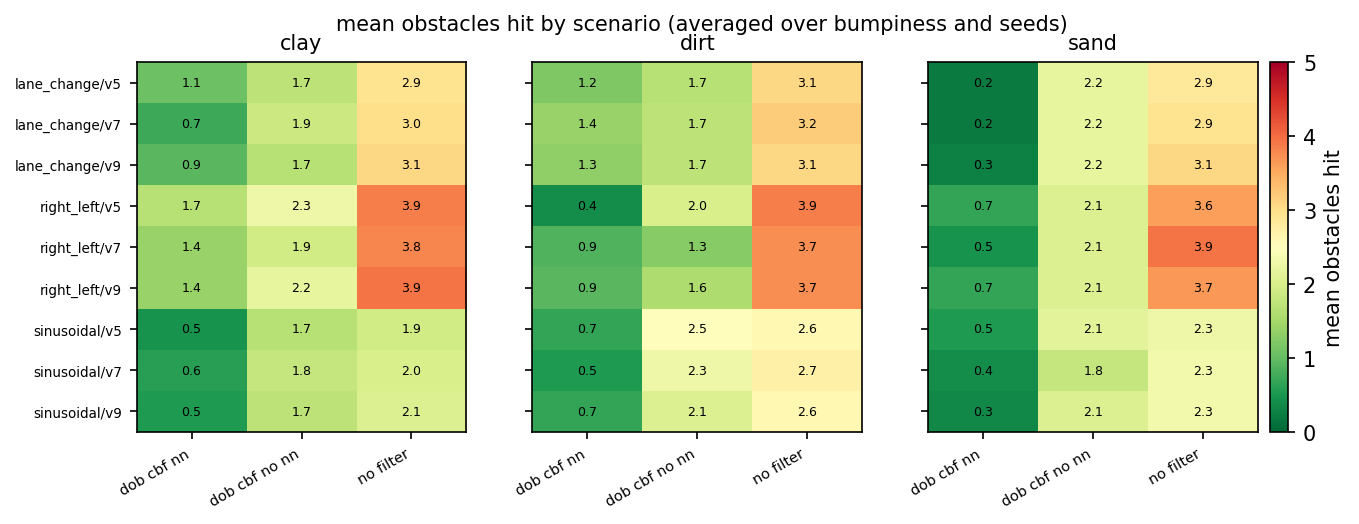
\includegraphics[width=\textwidth]{dob_cbf_nn_ablation_heatmap.png}
  \caption{DOB-CBF neural-surrogate ablation: per-scenario
    collisions. Aggregate KPIs are in Table~\ref{tab:dobcbf_nn}.}
  \label{fig:dobcbf_nn}
\end{figure*}

\subsection{Planner tire model under a fixed DOB-CBF filter}
\label{sec:safety_tire}

A separate sweep runs the autonomous obstacle scenario with the
DOB-CBF filter always on, varying only the planner's tire model (the
analytical planners use the SCM-calibrated parameters of
Sec.~\ref{sec:tires_static}). All three tire models avoid the obstacles
approximately equally
(Table~\ref{tab:auto_obstacle} and Fig.~\ref{fig:auto_obstacle}),
indicating that the safety filter dominates the filter-mediated outcome
and that the planner-tire choice is largely orthogonal to the
safety outcome.

\begin{table}[!t]
  \renewcommand{\arraystretch}{1.10}
  \caption{Autonomous obstacle avoidance, planner tire model swept
    under a fixed DOB-CBF filter (analytical planners SCM-calibrated).
    1215 runs (405 per model).}
  \label{tab:auto_obstacle}
  \centering
  \begin{tabular}{lccc}
    \toprule
    \textbf{Planner tire model} & \textbf{Coll./run} &
    \textbf{Clearance (m)} & \textbf{CTE (m)}\\
    \midrule
    Pacejka              & $0.65\!\pm\!0.97$ & $+0.83\!\pm\!1.99$ & $0.86$\\
    TMeasy               & $0.61\!\pm\!0.92$ & $+0.93\!\pm\!2.03$ & $0.91$\\
    NN rate-MLP          & $0.65\!\pm\!0.97$ & $+0.65\!\pm\!1.96$ & $0.90$\\
    \bottomrule
  \end{tabular}
\end{table}

\begin{figure*}[!t]
  \centering
  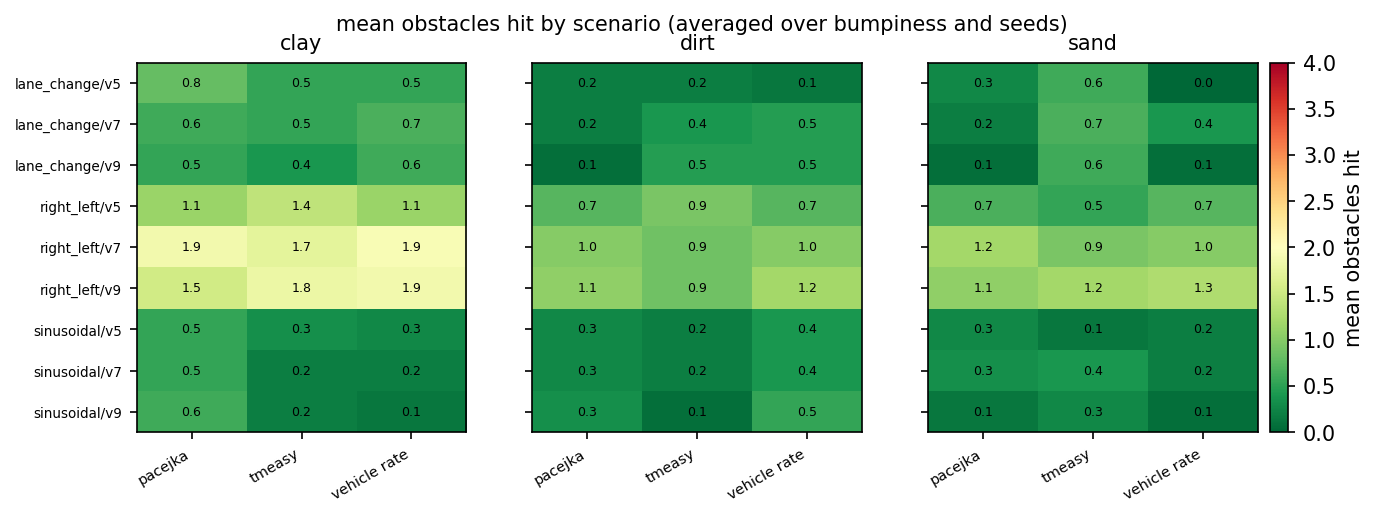
\includegraphics[width=\textwidth]{autonomous_obstacle_collision_heatmap.png}
  \caption{Autonomous obstacle avoidance, planner tire model swept
    under a fixed DOB-CBF filter. Mean unique obstacles hit per run
    stratified by terrain with across-seed whisker error bars; the
    three tire models are comparable here (their across-seed error bars
    overlap on every terrain) because the safety filter, not the
    planner-tire choice, dominates the safety outcome. Sweep matrix is clay/dirt/sand $\times$ 3 paths $\times$ 3
    speeds $\times$ 3 bumpiness $\times$ 5 seeds.
    Aggregate KPIs are in Table~\ref{tab:auto_obstacle}.}
  \label{fig:auto_obstacle}
\end{figure*}

\subsection{Counterfactual replay on dynamic-traffic (convoy) scenarios}
\label{sec:safety_convoy}

The evaluations above use static rock obstacles. To stress the filters
against \emph{dynamic} hazards we add PID-driven traffic vehicles --- full
HMMWVs sharing the ego's deformable-terrain system and collision world, each
following a lane at a set speed with scripted dangerous behaviour (a lead
vehicle braking, a cut-in, a vehicle stalled in the lane). They enter the same
obstacle interface as the rocks, so the ego planner and the safety filter must
avoid them with no change to either.

These scenarios enable the \emph{counterfactual} measurement that is this
paper's most direct filter-attribution result. Because Chrono replay is deterministic,
a fixed command trace is replayed through the \emph{identical}
scenario with the filter off and on, so every outcome difference is attributable
to the filter alone in a paired, reproducible collision-prevention measure
with no path-tracking proxy. To avoid resting the result on one input, the trace
is drawn from a small \emph{population of scripted worst-case commands}: a
``drive-into-the-hazard'' command at three throttle levels
($0.4$, $0.6$, $0.8$), a stand-in for an inattentive or
latency-overwhelmed operator. Table~\ref{tab:convoy_cf} aggregates these intents
across five convoy scenarios (lead-brake, 3- and 5-vehicle convoys,
rear-approach, stalled) $\times$ three command delays ($0$, $0.15$, $0.30\,$s)
for $45$ unfiltered baseline cells and $45$ completed DOB-CBF replays. The
unfiltered intent collides in $45$ of $45$ cells; DOB-CBF \emph{prevents $36$ of
the $45$ baseline collisions}, cutting the collision rate from $100\%$
to $20\%$ and turning a mean
clearance of $-2.23\,$m into $+2.25\,$m. It does so at small command deviation
($|\Delta\delta|=0.13$, $|\Delta\tau|=0.33$), mixing steering with braking ---
the obstacle-type-aware QP steers around static rocks but is willing to brake
behind a vehicle.

The same machinery replays a \emph{recorded} G29 trace unchanged, turning
logged human intent into a drop-in input. We replayed ten such drives ---
the five convoy scenarios under a good and a congested 5G profile
(Sec.~\ref{sec:latency}), driven glass-to-glass on the delayed camera and
command paths --- filter-off versus DOB-CBF (Fig.~\ref{fig:teleop_cf}).
The operator collided in five of the ten drives; DOB-CBF cut that to two
(three of five averted) and lifted the median minimum clearance from
$0.15$ to $4.42\,$m at small command deviation
($|\Delta\delta|\!\approx\!0.04$, $|\Delta\tau|\!\approx\!0.15$, near-inert
on the good link). It prevented all four \emph{forward}-collision cases
--- both convoys, the congested lead-brake, and the congested platoon
($-0.69\!\to\!+10.3\,$m).

The two residual collisions mark the filter's scope. One is a
rear-approach, which a forward-collision filter cannot prevent by
construction (the operator hit it too). The other is a congested
stalled-vehicle case where the filter braked to a near-stop instead of
committing to the operator's wide bypass; the resulting $0.5\,$m contact
is largely a replay artifact --- the filter runs $5\times$ slower than the
recorded drive, so the operator's post-pass steering, replayed on the
slowed vehicle, drifts it into the stall (a live operator would adapt).
These expose two real limits: the filter is over-conservative on a
stationary blocker under heavy delay, and open-loop replay loses fidelity
when the filter substantially alters the speed profile. On genuine human
intent the filter restores large clearance margins on the cases it is
designed for without fighting a capable driver (single operator; a
multi-operator study is future work).

\begin{table}[!t]
  \renewcommand{\arraystretch}{1.10}
  \caption{Counterfactual convoy replay: a population of scripted worst-case commands
    (constant throttle $\in\{0.4,0.6,0.8\}$ into the hazard) replayed
    filter-off vs DOB-CBF across 3 traffic scenarios $\times$ 5 command delays
    ($45$ cells per filter, all runs completed). The paired
    deterministic replay isolates collision prevention by the filter for these
    scripted intents.
    $|\Delta\delta|$, $|\Delta\tau|$ are the mean
    steering/throttle corrections.}
  \label{tab:convoy_cf}
  \centering
  \setlength{\tabcolsep}{3pt}
  \footnotesize
  \begin{tabular}{lccccc}
    \toprule
    \textbf{Filter} & \textbf{Coll.\ rate} & \textbf{Prevented} & \textbf{Clear.\,(m)} & $\mathbf{|\Delta\delta|}$ & $\mathbf{|\Delta\tau|}$\\
    \midrule
    None      & $1.00$ ($45/45$) & --- & $-2.23\!\pm\!0.96$ & --- & ---\\
    \textbf{DOB-CBF} & $\mathbf{0.20}$ ($9/45$) & $\mathbf{36/45}$ & $\mathbf{+2.25\!\pm\!1.95}$ & $0.13$ & $0.33$\\
    \bottomrule
  \end{tabular}
\end{table}

\begin{figure}[!t]
  \centering
  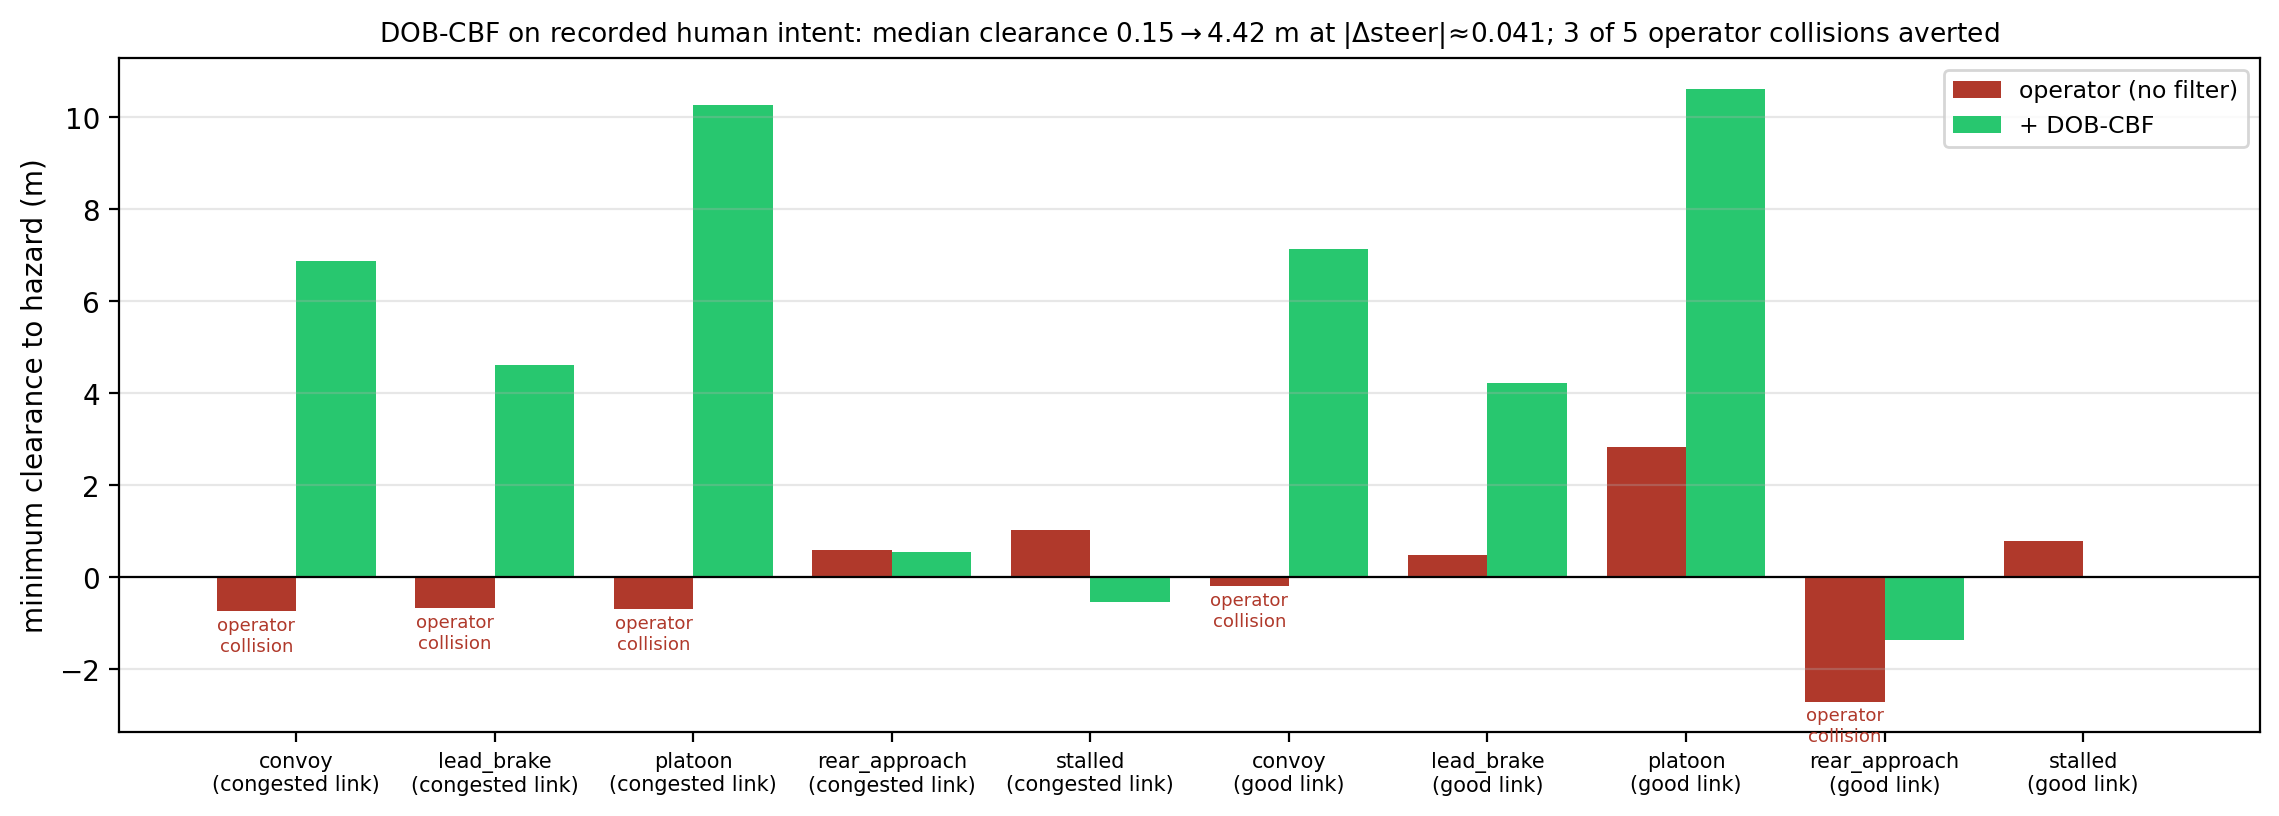
\includegraphics[width=\columnwidth]{teleop_counterfactual_clearance.png}
  \caption{Counterfactual replay on ten \emph{recorded human} G29 drives (five
    convoy scenarios $\times$ good/congested 5G latency, driven glass-to-glass on
    the delayed camera + command paths), operator (no filter) vs DOB-CBF. Under
    the hard delayed-video condition the operator collides in five of ten
    (clearance $<0$); DOB-CBF averts the four \emph{forward}-collision cases and
    lifts the median minimum clearance from $0.15$ to $4.42\,$m at
    $|\Delta\delta|\!\approx\!0.04$. Two residual collisions bound its scope: a
    rear-approach (a forward filter cannot prevent it) and one congested stalled
    case where the filter braked to a near-stop instead of swerving wide; that
    $0.5\,$m contact is largely an open-loop-replay artifact (operator steering
    replayed on the $5\times$-slower filtered vehicle), not a braking failure.}
  \label{fig:teleop_cf}
\end{figure}


\subsection{Real-time cost}
\label{sec:safety_scaling}

DOB-CBF is a single small quadratic program solved once per control tick.
Against the $100\,$ms ($10\,$Hz) control-tick budget its solve scales benignly with
the number of in-range obstacles $N$ (a rock and a traffic vehicle are
identical $(x,y,r)$ entries, so $N$ counts both): a fraction of a millisecond
at $N=0$ rising to only a few milliseconds at $N\!\sim\!100$. It therefore
never approaches the budget and imposes no practical obstacle-count limit ---
one reason it is well suited to the dense boulder-and-convoy scenes here.

%======================================================================
\section{5G-Profile Latency Robustness}
\label{sec:latency}
%======================================================================

A sequence model (N-HiTS) is trained on the public 5G YouTube
uplink dataset of Choi et al.~\cite{Choi23} and used to generate a
synthetic bitrate trace. The trace is mapped through a configurable
queue-load model to produce a per-channel latency profile that is
applied as an additive scheduled delay on the camera and command
channels (Fig.~\ref{fig:latency_profile}).

\begin{figure}[!t]
  \centering
  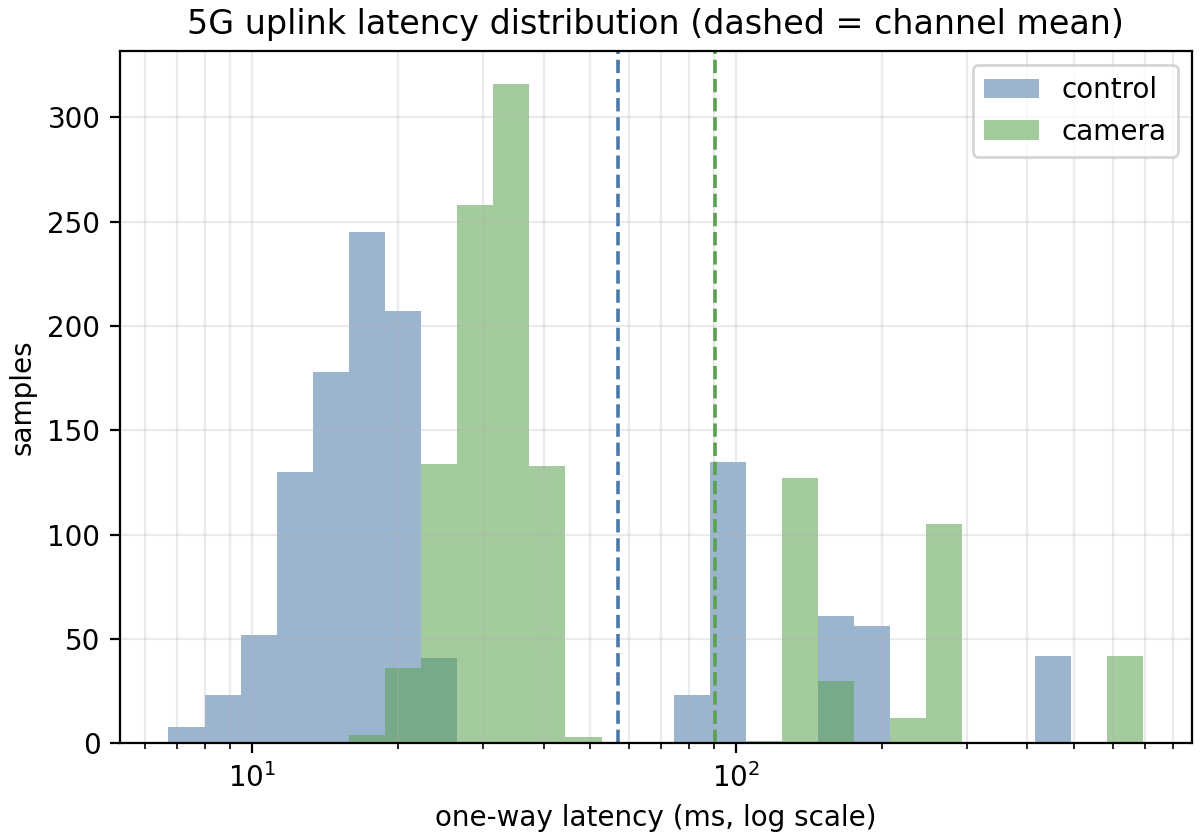
\includegraphics[width=\columnwidth]{latency_profile_histogram.png}
  \caption{Learned N-HiTS 5G uplink profile applied to the camera and
    control channels (log-$x$ histogram; dashed lines are channel
    means). The profile is bimodal: a low-latency bulk
    (control around $10$--$25\,\mathrm{ms}$, camera around
    $30$--$50\,\mathrm{ms}$), a higher-latency cluster near
    $100$--$200\,\mathrm{ms}$, and discrete outage spikes at
    $450\,\mathrm{ms}$ (control) and $660\,\mathrm{ms}$ (camera). Mean
    one-way latency is approximately $57\,\mathrm{ms}$ (control) and
    $91\,\mathrm{ms}$ (camera).}
  \label{fig:latency_profile}
\end{figure}

The closed-loop obstacle scenario is then run under the synthetic
profile with and without the safety filter; Table~\ref{tab:latency_comp}
and Fig.~\ref{fig:latency_comp} report the result.
Under the learned 5G profile DOB-CBF cuts collisions by $88\,\%$
($2.74\!\to\!0.34$ per run) and turns a negative mean clearance
($-1.45\,$m, inside the obstacle footprint) into $+0.41\,$m, intervening on
about half of the steps. The minimum-deviation, intent-preserving behaviour
that suits the human-in-the-loop case (Sec.~\ref{sec:safety}) thus holds up
even under the profile's outage spikes.

\begin{table}[!t]
  \renewcommand{\arraystretch}{1.10}
  \caption{Closed-loop collisions under the learned N-HiTS-5G
    latency profile (DOB-CBF vs no filter).}
  \label{tab:latency_comp}
  \centering
  \begin{tabular}{lccc}
    \toprule
    \textbf{Filter} & \textbf{Coll./run} & \textbf{Clearance (m)} & \textbf{Interv. (\%)}\\
    \midrule
    None      & $2.74\!\pm\!1.17$ & $-1.45\!\pm\!0.60$ & ---\\
    \textbf{DOB-CBF}   & $\mathbf{0.34\!\pm\!0.57}$ & $\mathbf{+0.41\!\pm\!1.10}$ & $52$\\
    \bottomrule
  \end{tabular}
\end{table}

\begin{figure*}[!t]
  \centering
  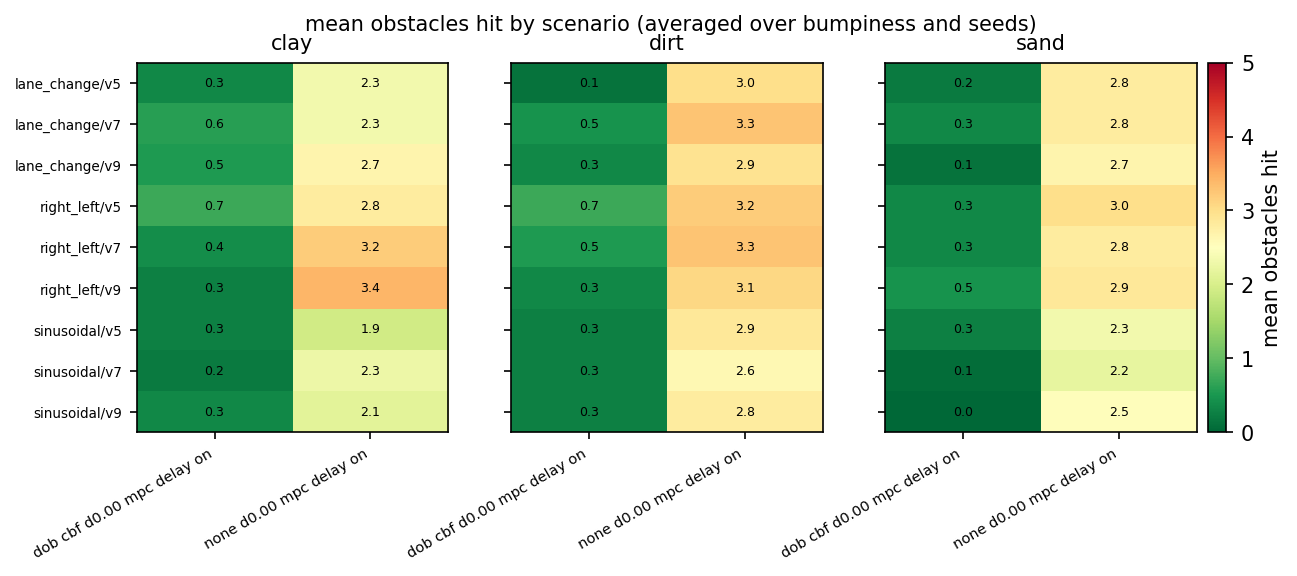
\includegraphics[width=\textwidth]{latency_compensation_collision_heatmap.png}
  \caption{5G-profile latency compensation sweep: per-scenario
    collisions. Aggregate KPIs are in Table~\ref{tab:latency_comp}.}
  \label{fig:latency_comp}
\end{figure*}

\subsection{Isolating the value of delay-awareness}
\label{sec:latency_ablation}

The result above shows a filter helps under latency, but not that the filter's
\emph{delay compensation} --- inflating its obstacle buffer by a
delay-dependent stopping distance and forward-predicting over the round trip
before acting --- is what helps, rather than merely screening the command at
all. We isolate it with a deterministic ablation: the command path is delayed
by $\Delta_\mathrm{cmd}$ in \emph{every} run, but the filter is either
\emph{told} the delay (``aware'') or not (``blind''); everything else
is identical, and the same scripted worst-case commands (Sec.~\ref{sec:safety_convoy})
are replayed, so blind-vs-aware is paired. We sweep it as a dose-response over
six command delays ($0$ to $0.5\,$s) $\times$ $5$ convoy scenarios $\times$ three
intents ($90$ cells per variant). Both filters reduce collisions substantially
relative to no filter ($0.87$), but the delay-aware filter is strictly better
overall: a $0.17$ collision rate vs the delay-blind $0.26$, at twice the
clearance margin ($+2.34$ vs $+1.16\,$m), preventing $8$ of the blind filter's
collisions on matched cells. Crucially the gap \emph{grows with delay}
(Fig.~\ref{fig:latency_ablation}): at $\Delta_\mathrm{cmd}\!=\!0$ the two are
identical ($0.33$ each --- the sanity check, since with no delay there is
nothing to be aware of), by $0.30\,$s the delay-blind filter still collides at
$0.20$ while the aware filter is down to $0.07$, and by $0.50\,$s awareness
removes the residual entirely ($0.20\!\to\!0.00$). Intrusiveness is comparable
either way ($|\Delta\delta|\!\approx\!0.10$--$0.14$), so the gain is smarter
timing, not more aggression. This supports the \emph{latency-aware} claim
specifically, rather than only showing generic latency robustness.

\begin{figure}[!t]
  \centering
  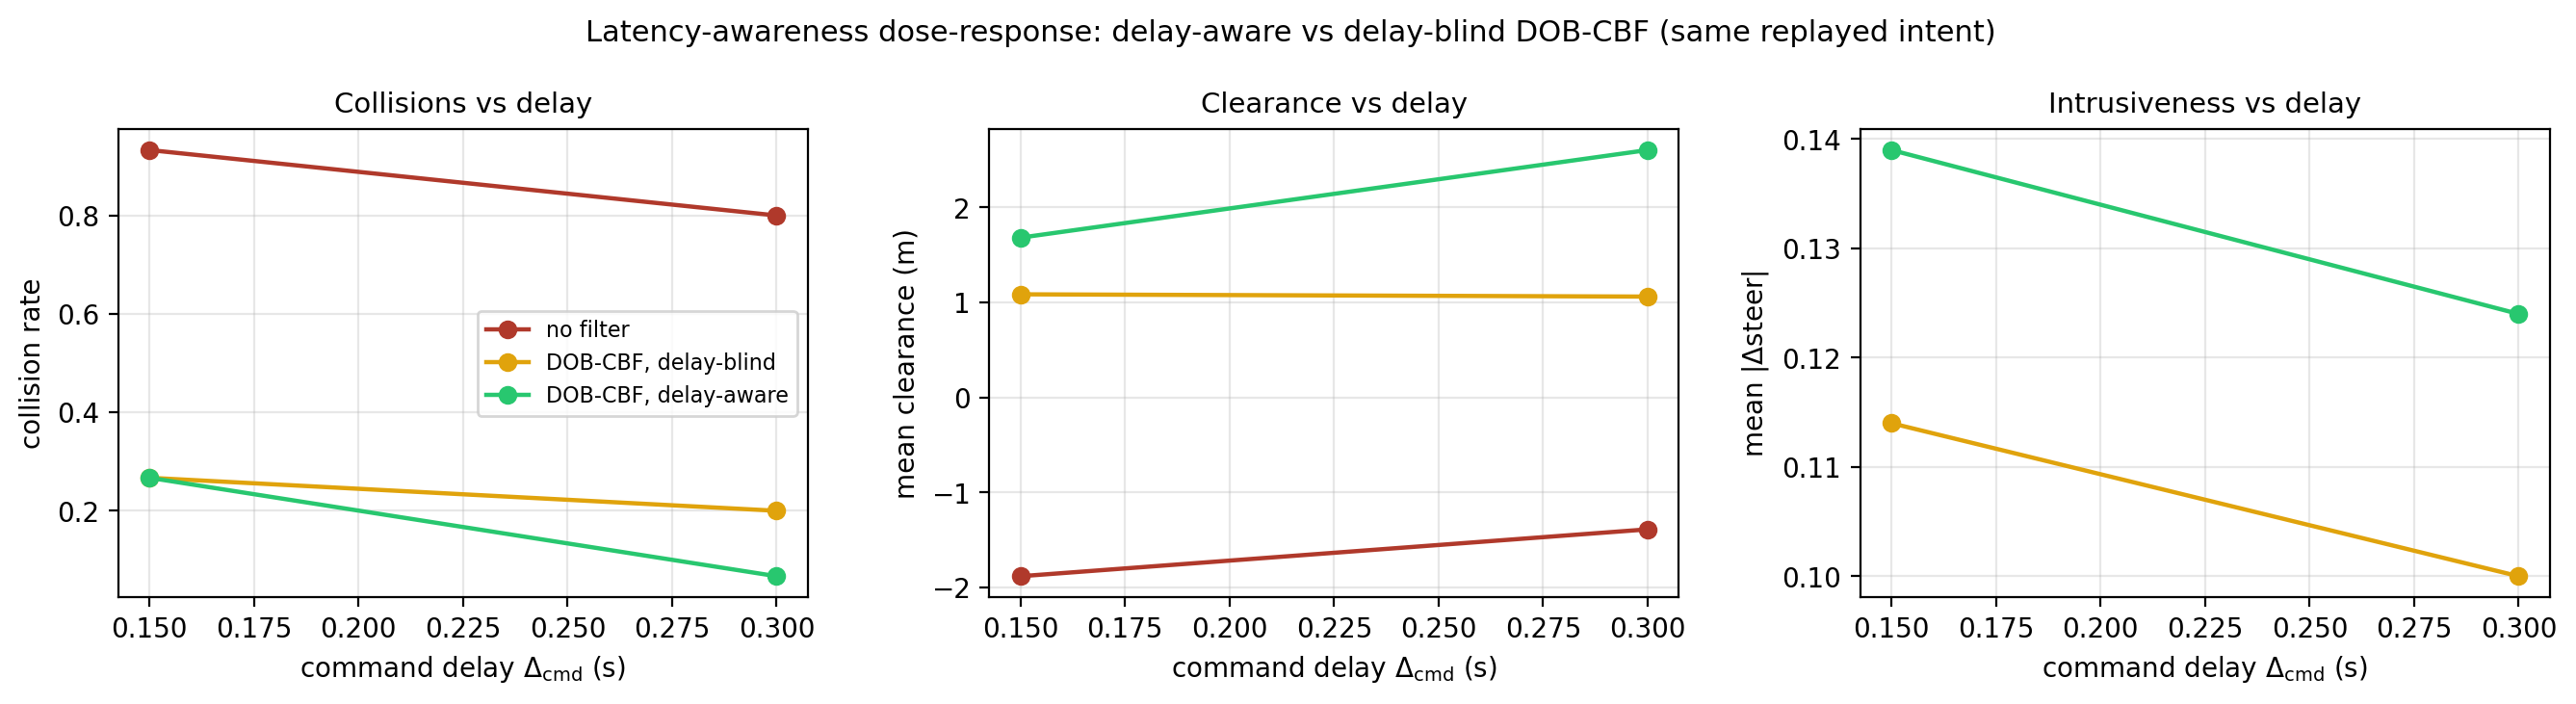
\includegraphics[width=\columnwidth]{latency_awareness_ablation.png}
  \caption{Latency-awareness dose-response. The same scripted worst-case commands are
    replayed with the command path delayed by $\Delta_\mathrm{cmd}$, the DOB-CBF
    filter either \emph{told} that delay (aware) or not (blind), swept over six
    delays. At zero delay the two coincide (nothing to be aware of); the gap
    grows with delay --- by $0.5\,$s awareness removes the residual collisions
    the delay-blind filter still suffers, at comparable intrusiveness. $90$
    deterministic cells per variant.}
  \label{fig:latency_ablation}
\end{figure}

%======================================================================
\section{Terrain- and Latency-Aware Collision Warning}
\label{sec:collision_warning}
%======================================================================

The safety filter in
\S\ref{sec:safety}--\S\ref{sec:latency} modifies the
operator's command stream when a collision is imminent. In some
deployment modes (e.g. expert-loop teleoperation, or a safety filter
that has been muted for debugging) the operator wants only a
\emph{notification} rather than a control override. We add an
independent forward collision warning component that runs in parallel
with the rest of the stack and emits a discrete severity signal
$\{\textsc{green}, \textsc{yellow}, \textsc{orange}, \textsc{red}\}$
on every controller tick, escalating as the vehicle closes on a hazard
(Fig.~\ref{fig:warning_ui}). The signal drives the operator's heads-up
overlay --- a severity banner, the current clearance against the required
stopping distance, and the live terrain-conditioned brake budget;
Fig.~\ref{fig:cw_timeline} traces the escalation over a full approach.

\begin{figure}[!t]
  \centering
  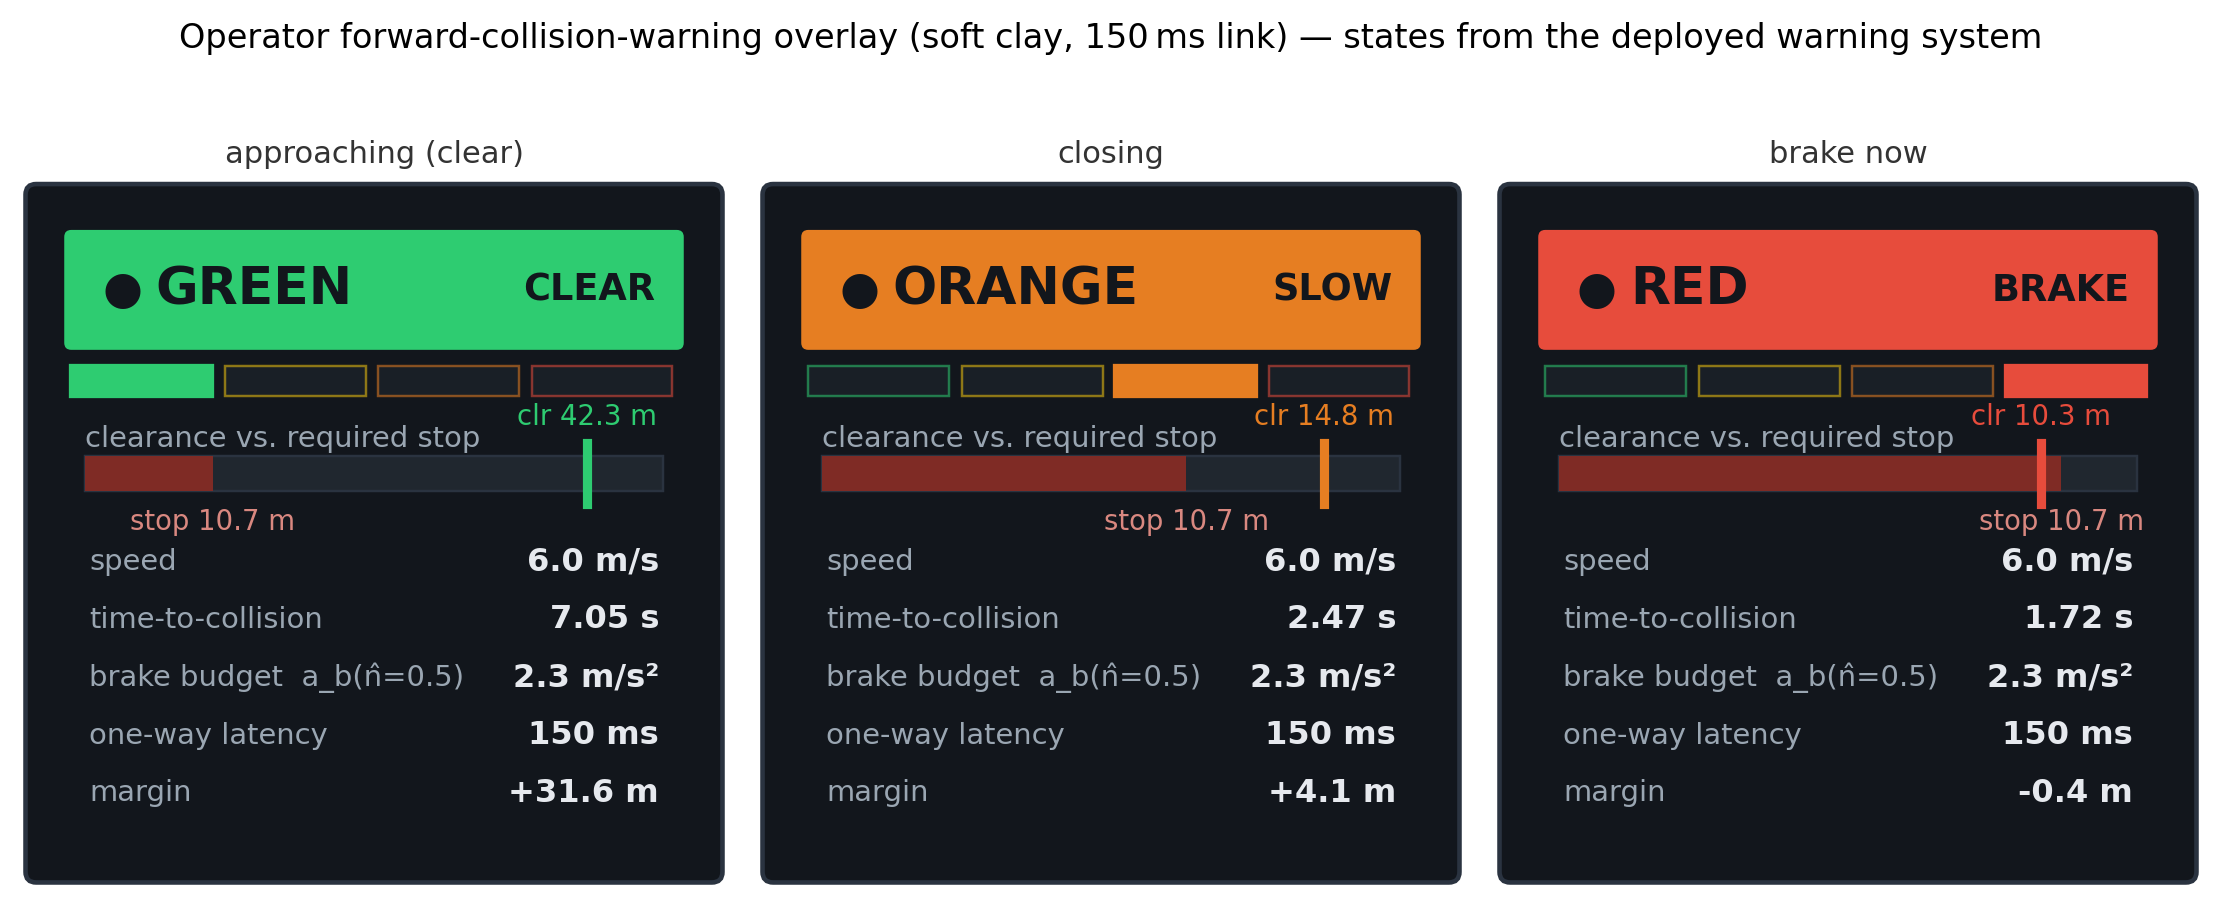
\includegraphics[width=\columnwidth]{warning_ui.png}
  \caption{The operator's forward-collision-warning overlay at three moments of
    a straight-in approach on soft clay under a $150\,\mathrm{ms}$ link,
    escalating \textsc{green}$\to$\textsc{orange}$\to$\textsc{red}. The severity
    ladder, time-to-collision, clearance-versus-required-stop bar, and the
    terrain-conditioned brake budget $a_b(\hat n)$ are the live outputs of the
    deployed warning system (not a mock-up); \textsc{red} fires once the margin
    (clearance $-$ required stopping distance) crosses zero.}
  \label{fig:warning_ui}
\end{figure}

The warning module is exposed through a small factory in line with
the rest of the swappable safety layer, so the warning strategy can
be selected at construction time. The default strategy is a
time-to-collision predictor with two adjustments:

\paragraph{Terrain awareness.} The required stopping distance
$d_{\mathrm{stop}}=v\tau_{r}+v^{2}/(2a_{b})$ uses a brake-deceleration
$a_{b}(\hat n)$ that is computed \emph{analytically at init time} by
querying the same rig tire surrogate the
DOB-CBF and MPC use for traction-budget queries. For every $\hat n
\in [0.40,1.30]$ on a 0.05 grid, the surrogate is loaded with the
manifold-interpolated Bekker vector at that $\hat n$, swept over
braking slip ratios $\kappa\in[-0.40,0]$ at static per-wheel $F_z$,
and the peak $|F_x|$ at front and rear axles is summed to give the
total available braking force; $a_b(\hat n)=\sum F_{x,\mathrm{peak}}
/ m_{\mathrm{veh}}$. The resulting table runs from
$a_b(0.4)\!\approx\!2.3\,\mathrm{m/s^{2}}$ (soft, clay-like) to
$a_b(1.1)\!\approx\!4.7\,\mathrm{m/s^{2}}$ (firm, sand-like) --- both
endpoints noticeably more conservative than a hand-tuned
$2.5/6.0\,\mathrm{m/s^{2}}$ heuristic. The live $\hat n$ from the online terrain estimator
(\S\ref{sec:estimator}) indexes into this table at runtime, so the
warning is more conservative on soils that the vehicle cannot brake
hard on.

\paragraph{Brake-decel validation.}
The analytical $a_b(\hat n)$ table is validated against actual Chrono
SCM behaviour with 27 full-brake stops: three terrains $\times$
three initial speeds $\{3,5,7\}\,\mathrm{m/s}$ $\times$ three seeds,
each scenario cruising to target speed and then applying
$\mathrm{brake}=1$, $\mathrm{throttle}=0$ until the vehicle is below
$0.2\,\mathrm{m/s}$. Stopping distance and mean decel are extracted
from the recorded chassis trajectory and compared to the prediction
at the brake-onset speed (Fig.~\ref{fig:cw_brake_validation}). On
mean decel, the rig-NN analytical table is within $0.1\,\mathrm{m/s^{2}}$
on clay, over-predicts dirt by $0.7\,\mathrm{m/s^{2}}$ (the
classical contact-patch saturation gap of \S\ref{sec:tires_rig_vs_vehicle}),
and over-predicts sand by $1.1\,\mathrm{m/s^{2}}$ --- small enough
that the resulting stopping-distance prediction lands within
$\pm 0.5\,\mathrm{m}$ of the recorded ground truth on 23 of 27
trials. Aggregated mean $|\Delta d_{\mathrm{stop}}|$ is
$0.17\,\mathrm{m}$ for the analytical table versus $0.45\,\mathrm{m}$
for the hand-tuned linear-interp fallback ($2.6\times$ improvement);
the analytical prediction also has a small positive mean bias
($+0.10\,\mathrm{m}$), meaning the warning is biased toward firing
slightly earlier than strictly necessary, which is the safe
direction.

\begin{figure*}[!t]
  \centering
  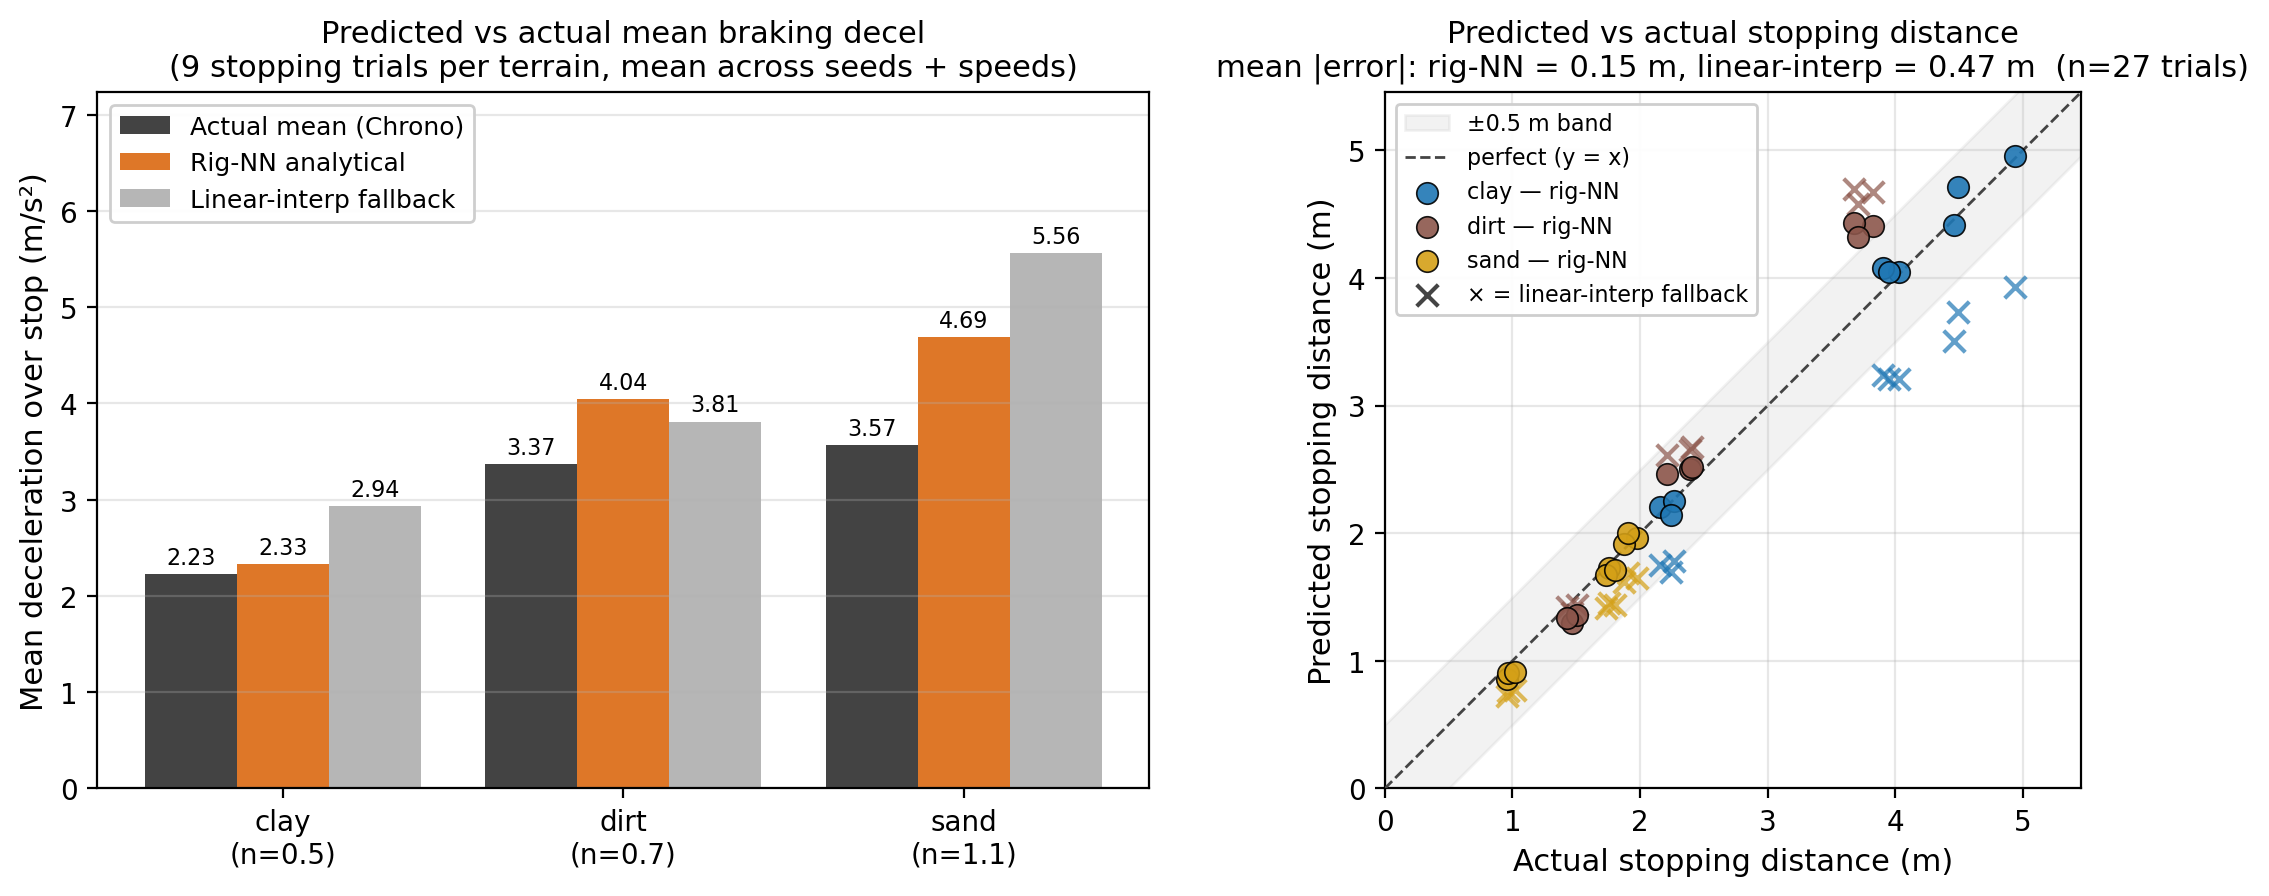
\includegraphics[width=\textwidth]{cw_brake_validation.png}
  \caption{Validation of the warning system's analytical
    brake-deceleration table against actual Chrono SCM stopping
    behaviour (27 trials, 3 terrains $\times$ 3 initial speeds
    $\times$ 3 seeds). Left: mean deceleration over each stop. The
    rig-NN analytical estimate (orange) matches the Chrono mean
    (black) closely on clay and slightly over-predicts on dirt and
    sand; the original linear-interp fallback (grey) under-predicts
    on clay and over-predicts on sand. Right: predicted vs actual
    stopping distance with the $\pm 0.5\,\mathrm{m}$ band shaded.
    Rig-NN points (circles) cluster tighter to $y=x$ than
    linear-interp ($\times$, scatter); mean $|\Delta d_{\mathrm{stop}}|$
    is $0.17\,\mathrm{m}$ analytical vs $0.45\,\mathrm{m}$
    linear-interp.}
  \label{fig:cw_brake_validation}
\end{figure*}

\begin{figure*}[!t]
  \centering
  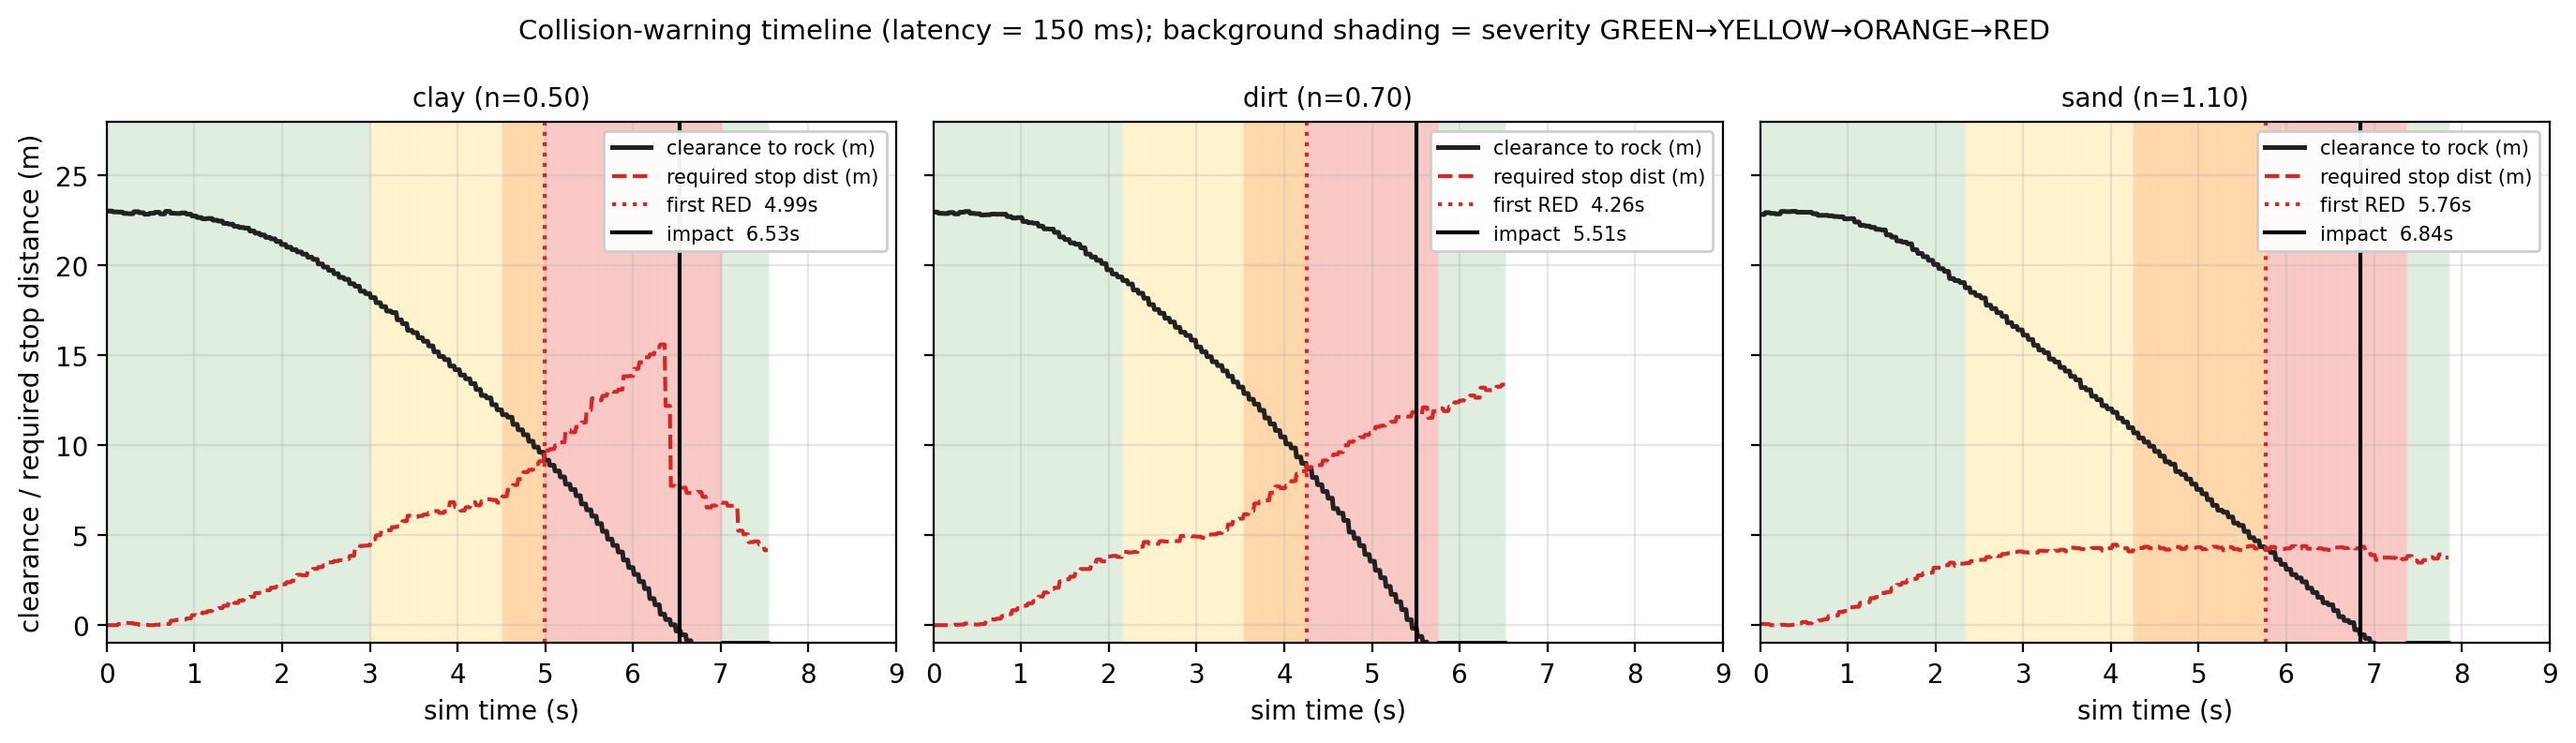
\includegraphics[width=\textwidth]{cw_timeline.png}
  \caption{Severity escalation over time for one representative
    blind-drive run per terrain at $150\,\mathrm{ms}$ one-way delay.
    Background shading is the live severity band (GREEN $\to$ YELLOW
    $\to$ ORANGE $\to$ RED); curves are the chassis clearance to the
    rock (solid) and the warning system's running stopping-distance
    estimate (dashed). The first RED fires when the clearance curve
    drops to the stopping-distance curve.}
  \label{fig:cw_timeline}
\end{figure*}

\paragraph{HIL integration.}
The warning module is wired through the sim node so any HIL
teleoperation round can enable it. Per-tick severity is logged
alongside the existing diagnostics, and severity transitions are
reported on the sim-node console and, when the Irrlicht visualiser
is active, surfaced to the operator as a text banner. When the
online terrain estimator is active, the live $\hat n$ is forwarded
to the warning system on every control message so that the
brake-decel estimate adapts to the estimator's current terrain
belief; otherwise the warning falls back to the nominal $n$ of the
configured terrain preset. The warning never modifies commands, so
it composes freely with the safety filter (none or DOB-CBF) used in
the same round.

\paragraph{Latency awareness.} An EMA tracker of recent one-way
network delays and a sliding-window jitter estimator inflate the
operator reaction time by $\tau_{r}\!+\!\mathrm{RTT}\!+\!k\sigma$,
where $\sigma$ is the standard deviation of one-way delays over the
last second of received commands. Increasing the latency baseline or
the jitter inflates $d_{\mathrm{stop}}$ and fires the warning
earlier.

\begin{figure}[!t]
  \centering
  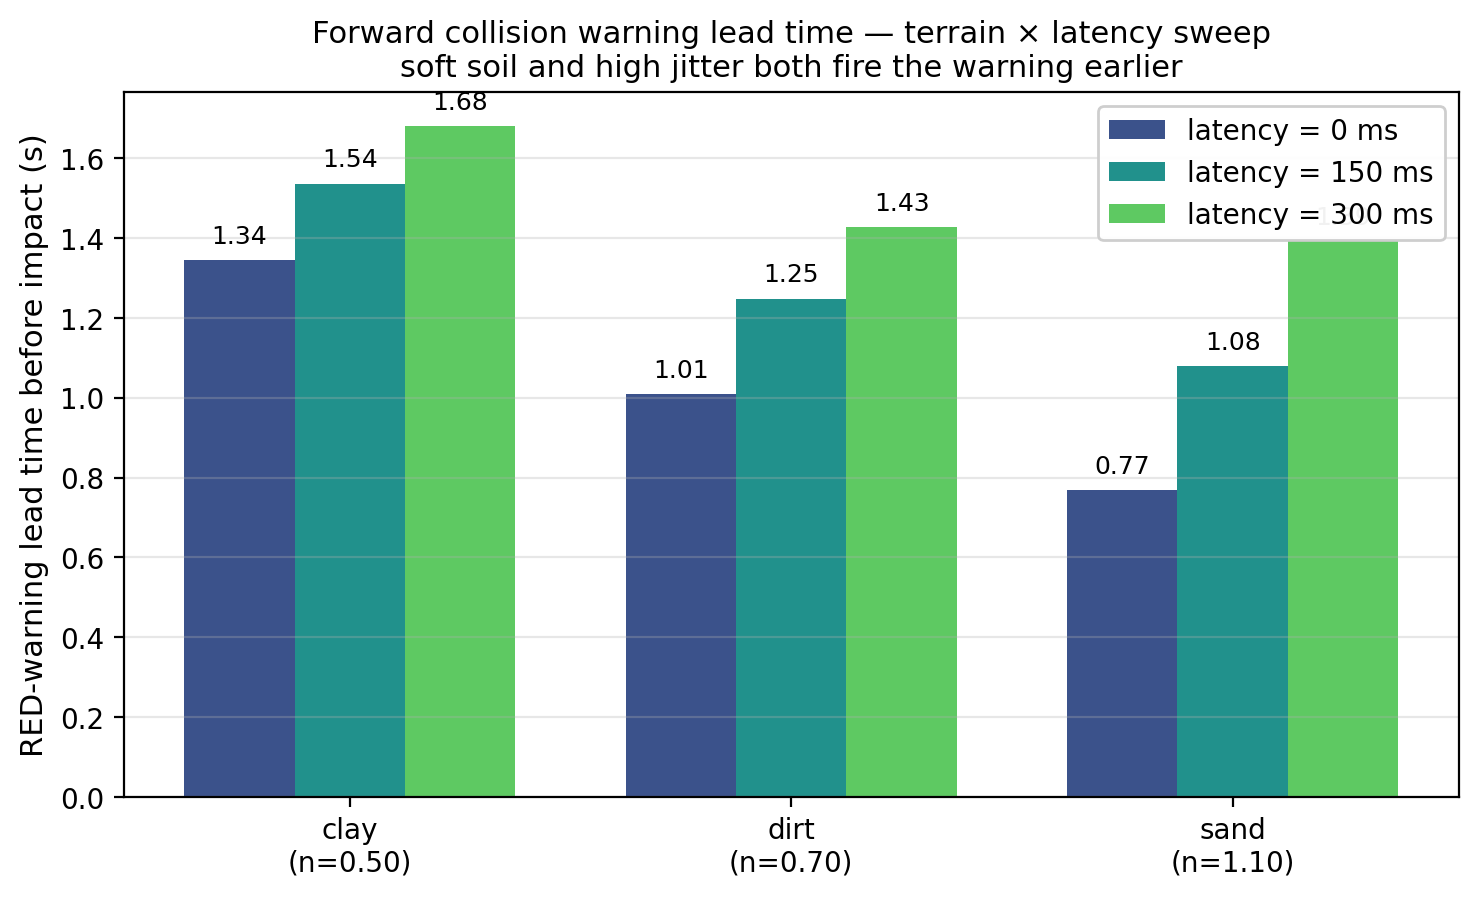
\includegraphics[width=\columnwidth]{cw_lead_vs_terrain.png}
  \caption{Forward collision warning lead time before impact in the
    blind-drive sweep (no MPC, no safety filter, fixed throttle into a
    single rock). Both the terrain-conditioned brake budget and the
    latency-conditioned operator-reaction budget enlarge the required
    stopping distance and therefore advance the first RED warning:
    soft soil (clay) gets the longest lead, and within every terrain
    the lead grows monotonically with the configured one-way delay.}
  \label{fig:cw_lead}
\end{figure}

\begin{table}[!t]
  \renewcommand{\arraystretch}{1.10}
  \caption{Forward collision warning lead time before impact (RED
    severity) under terrain $\times$ latency sweep. The vehicle drives
    blindly at a single $1.2\,\mathrm{m}$ rock with constant throttle.
    Higher latency and softer soil both increase the lead time, as
    designed.}
  \label{tab:cw_lead}
  \centering
  \begin{tabular}{lccc}
    \toprule
     & \textbf{lat=0\,ms} & \textbf{lat=150\,ms} & \textbf{lat=300\,ms}\\
    \midrule
    clay ($\hat n\!=\!0.5$) & $1.42\,\mathrm{s}$ & $1.58\,\mathrm{s}$ & $1.73\,\mathrm{s}$\\
    dirt ($\hat n\!=\!0.7$) & $1.03\,\mathrm{s}$ & $1.25\,\mathrm{s}$ & $1.42\,\mathrm{s}$\\
    sand ($\hat n\!=\!1.1$) & $0.77\,\mathrm{s}$ & $1.06\,\mathrm{s}$ & $1.33\,\mathrm{s}$\\
    \bottomrule
  \end{tabular}
\end{table}

The benchmark
sweeps three terrains and three one-way latency settings.
Table~\ref{tab:cw_lead} reports the time between the first
\textsc{red} warning and the rock impact: on soft clay the warning
fires approximately $1.42\text{--}1.73\,\mathrm{s}$ before impact; on firm
sand the same vehicle reaches the rock with about $0.77\text{--}1.33\,\mathrm{s}$
of lead. The lead time also grows with the configured operator
latency on every terrain (Fig.~\ref{fig:cw_lead}) (clay $1.42\!\to\!1.73\,\mathrm{s}$ as
latency goes $0\!\to\!300\,\mathrm{ms}$, dirt $1.03\!\to\!1.42$, sand
$0.77\!\to\!1.33$), confirming that the warning correctly couples both
the terrain-conditioned stopping budget and the latency-conditioned
operator-reaction budget.

%======================================================================
\section{Open-Source Benchmarking Suite}
\label{sec:suite}
%======================================================================

A single invocation of the suite's top-level driver executes all of
the autonomous sub-sweeps that produce the non-HIL results reported
in this paper, then merges the resulting figures and CSVs into the
publication set. The paper tier completes $25$ experiments and
$\approx\!11{,}900$ Chrono closed-loop trials on a single
24-core workstation (Fig.~\ref{fig:benchmark_suite}); the
human-in-the-loop protocol of Sec.~\ref{sec:safety_hil} is run separately
because it requires an operator at the wheel.

\begin{figure}[!t]
  \centering
  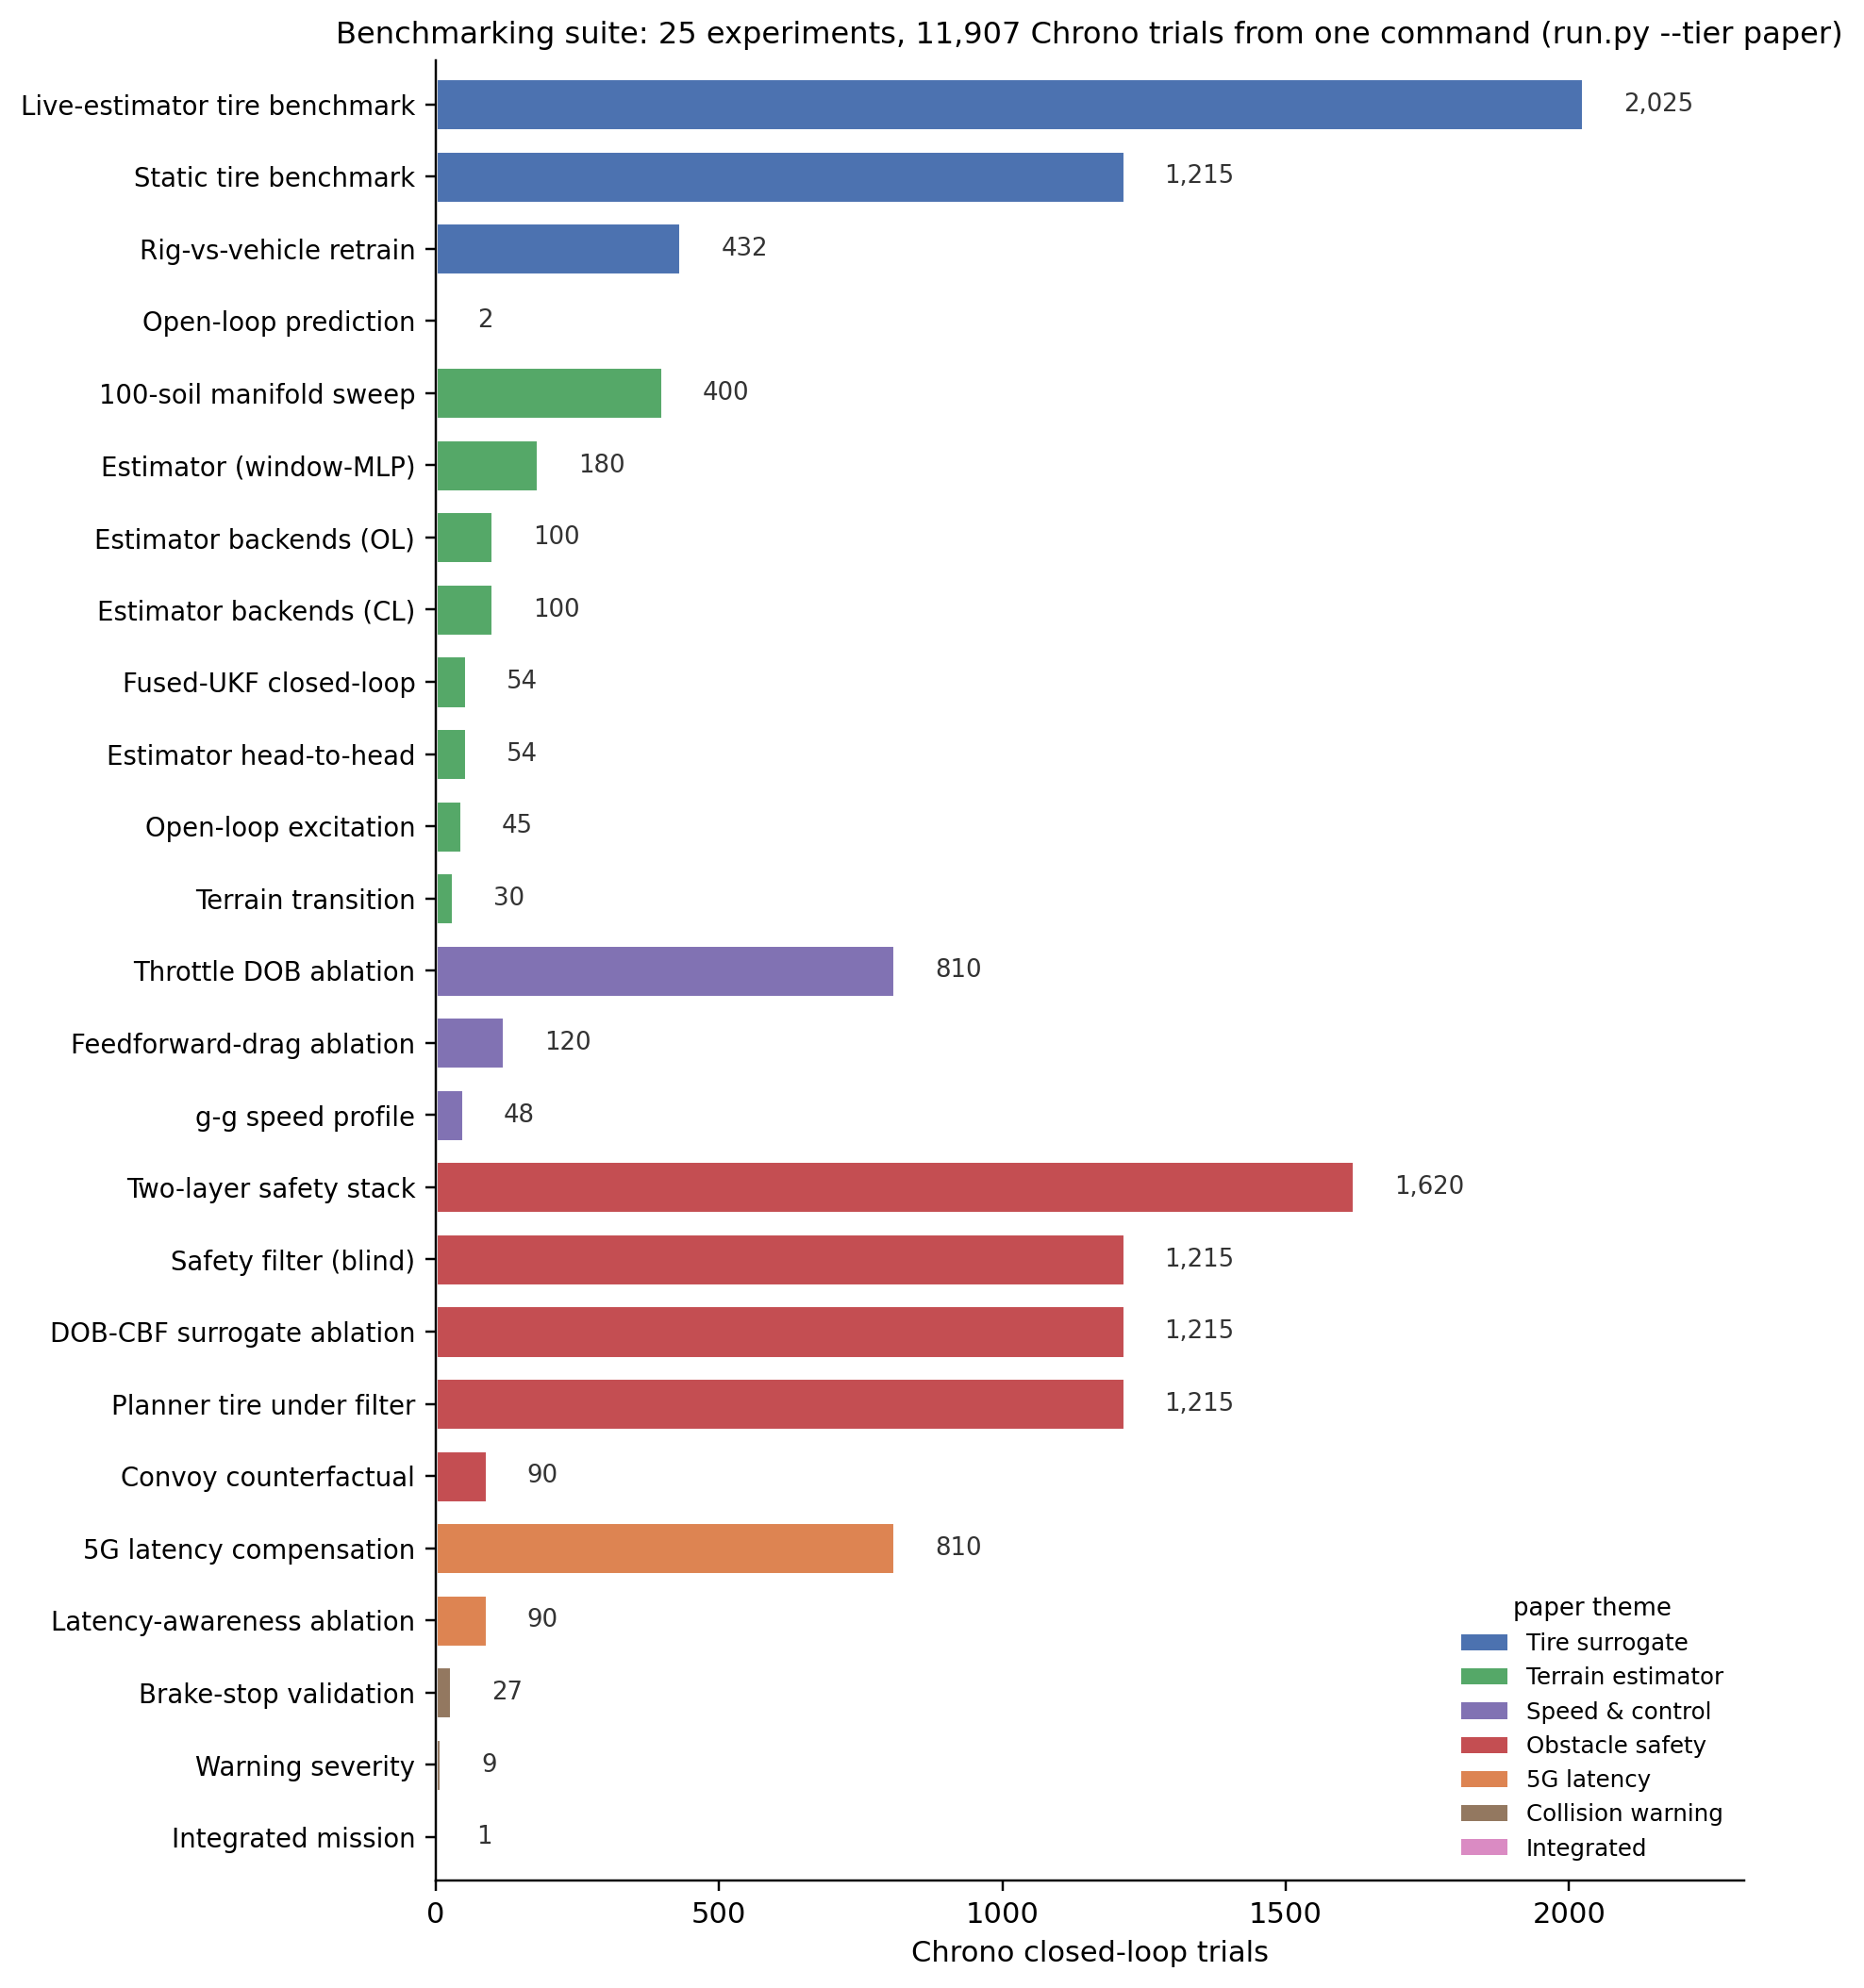
\includegraphics[width=\columnwidth]{benchmark_suite.png}
  \caption{Coverage of the open-source benchmarking suite: every closed-loop
    experiment run by \texttt{run.py -{}-tier paper}, coloured by the paper theme
    it backs, with its Chrono-trial count. One command reproduces $25$
    experiments and $\approx\!11{,}900$ trials; the counts are read directly from
    the suite's own run manifest.}
  \label{fig:benchmark_suite}
\end{figure}

Reproducibility is enforced through a few architectural
choices in the suite itself. Sensor noise is enabled in every trial
so no oracle quantity is observable at inference time. A per-trial
diagnostic CSV is saved alongside each run for post-hoc inspection.
Aggregated KPIs deduplicate on the run key
$(\textit{variant},\,\textit{terrain},\,\textit{path},\,\textit{speed},\,
\textit{bumpiness},\,\textit{seed})$, so a re-run cleanly fills only
the missing cells without overwriting existing rows. Parallel sweep
workers are isolated by a per-run ROS~2 domain, and the publication step
matches result folders by exact timestamp so that closely-named sweep
variants are never conflated.

%======================================================================
\section{Integrated System Demonstration}
\label{sec:integrated}
%======================================================================

The preceding sections evaluate each layer in isolation on shared
infrastructure; the contribution, however, is their \emph{integration}. As a
capstone we run the entire stack together on a single mission and present it as
one timeline (Fig.~\ref{fig:hero}): a sinusoidal reference driven across a
clay\,$\to$\,sand soil transition through a rock field, under the learned 5G
command/camera latency, with the terrain-aware NMPC, the online Fused-UKF
terrain estimator, the g--g speed planner, the throttle DOB, the DOB-CBF safety
filter, and the forward collision warning all active simultaneously. The online
estimate $\hat n$ adapts across the soil boundary (top); the achieved speed
tracks the grip-limited g--g reference with the DOB closing the soft-soil gap
(middle); and the safety filter keeps the traverse \emph{collision-free}
(closest pass $0.02\,$m at the tightest rock, $111$ binding-constraint
avoidance steps) over the $148\,$m mission (bottom). Running the full
stack is itself an integration test: it exercises the cross-layer interfaces
that per-component evaluation does not --- here the estimator's live-terrain
update re-conditions the safety filter's grip-limited braking authority, the
same topic the controller uses to re-condition its own surrogate. The run is
reproduced by \texttt{benchmarking/integrated\_hero\_run.py}. This single run
is an integration check rather than a separate statistical safety claim.

\begin{figure}[!t]
  \centering
  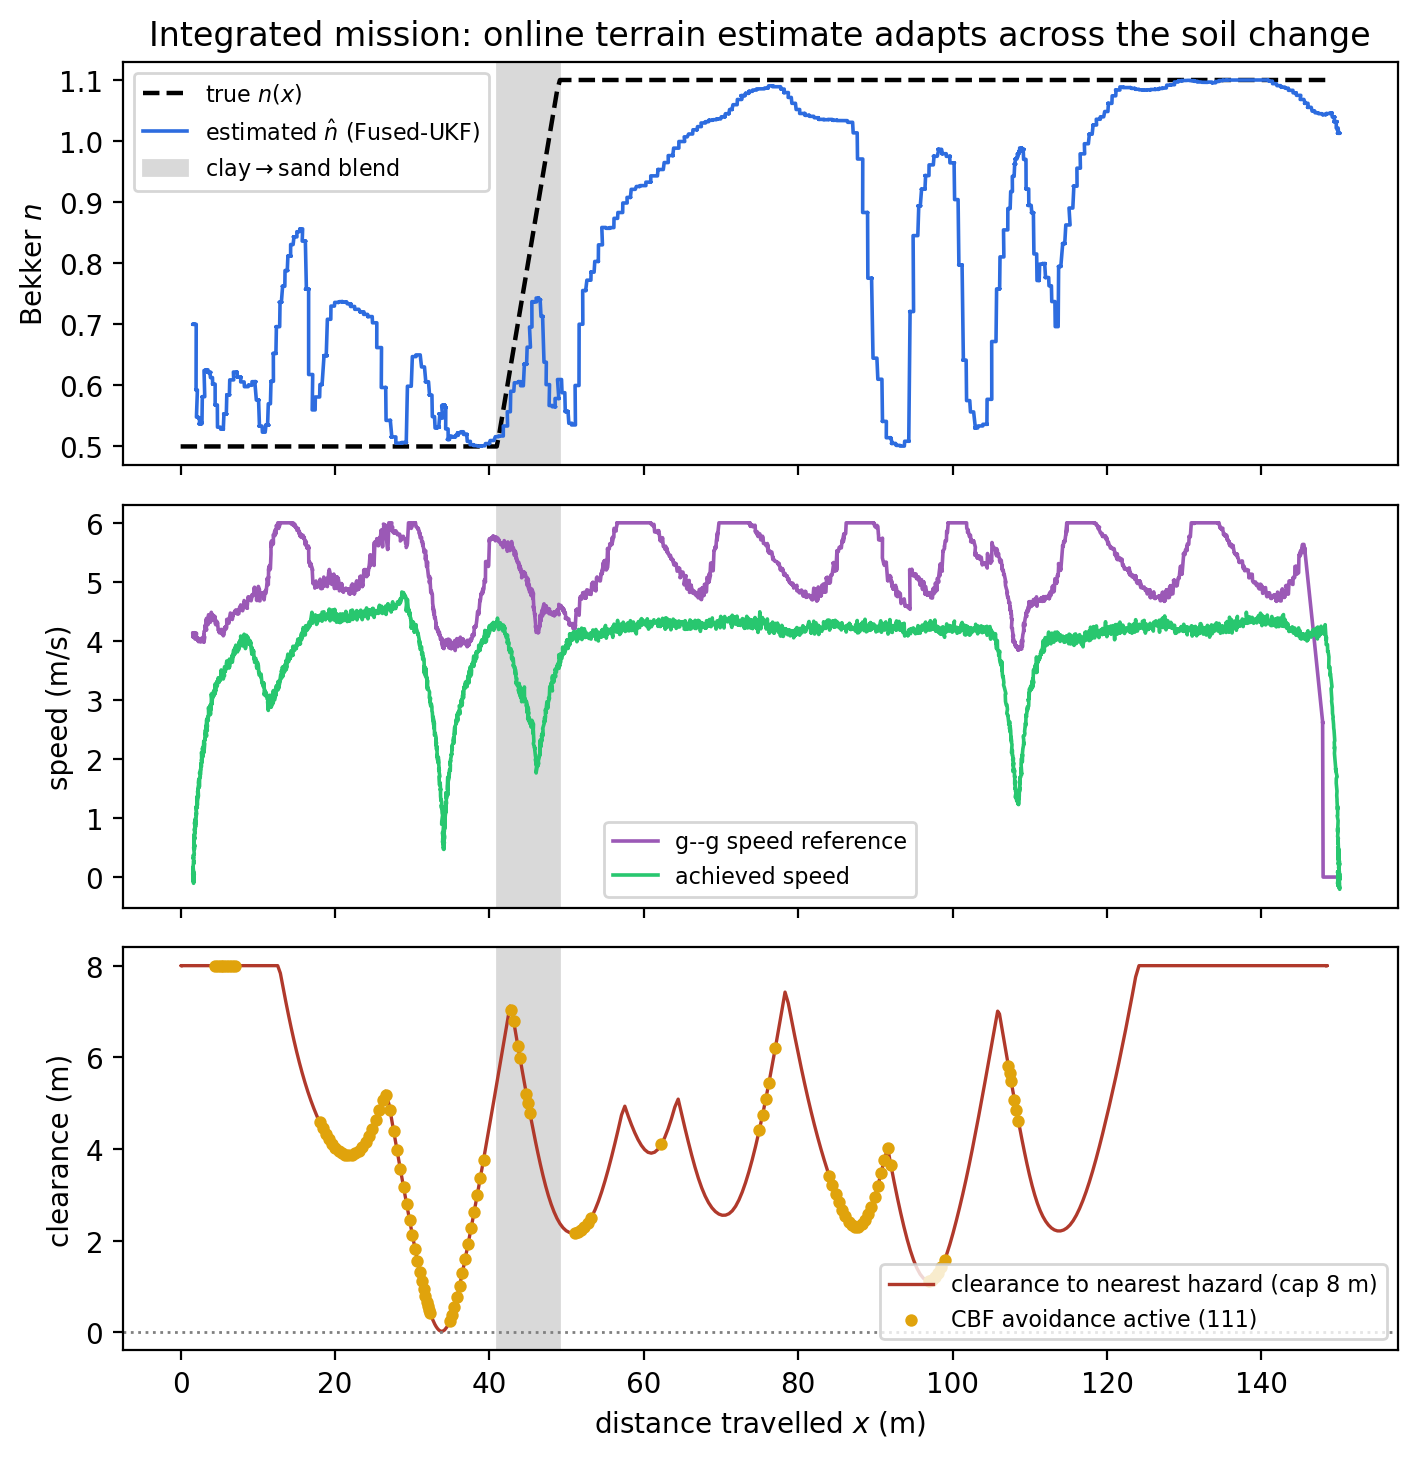
\includegraphics[width=\columnwidth]{integrated_hero_run.png}
  \caption{Integrated mission: the whole stack on one run, under the learned 5G
    latency, across a clay\,$\to$\,sand soil change (grey band) through a rock
    field. \textbf{Top:} the online terrain estimate $\hat n$ (blue) tracks the
    true $n(x)$ (dashed) across the soil boundary. \textbf{Middle:} achieved
    speed (green) tracks the terrain-aware g--g reference (purple). \textbf{Bottom:}
    clearance to the nearest hazard (capped at $8\,$m) dips at each rock, with
    the DOB-CBF binding-constraint avoidance steps marked; zero collisions over
    the traverse.}
  \label{fig:hero}
\end{figure}

%======================================================================
\section{Discussion}
\label{sec:disc}
%======================================================================

Two recent threads are directly adjacent to this framework.
Onozuka et al.~\cite{Onozuka25} replace a terrain-parameter-dependent NN
tire model with a physics-informed structure --- a Janosi saturating
shear law wrapped around two small networks that supply the force
coefficients --- re-fit online by gradient descent on state-derivative
residuals. The approach is complementary to ours: they fold soil
mechanics into a structured force law, whereas we estimate the soil and
re-condition an unstructured surrogate. Adapting their tire model into
our per-axle acados interface improved offline force prediction
($R^2_{F_y}$ from $0.35$ to $0.59$) but did not run stably in our
in-horizon NMPC, where the static formulation triggered QP failures on
aggressive transients; since their model targets a dedicated
curvilinear-coordinate, wheelspeed-state MPC we did not reimplement, this
is a note on complementarity, not a comparison. Gupta
et al.~\cite{Gupta24} compensate unmodeled dynamics with a
reinforcement-learning residual on top of MPC; on this plant such a
residual closed less than $8\,\%$ of the tracking error and only at the
largest model mismatch, so we do not adopt RL compensation.

The empirical evidence supports the central integration claim and the principal
component choices. The
whole-vehicle neural tire surrogate averages
$13.4\,\mathrm{ms}$ in the static tire-model sweep and
$13.2\,\mathrm{ms}$ in the live-estimator sweep (both within the
$100\,\mathrm{ms}$ MPC step) and reduces median RMS crosstrack error against the
\emph{SCM-calibrated} analytical baselines by $39$--$41\,\%$ in the
live-estimator regime (Table~\ref{tab:tires_estimator}), separating
clearly from them in the tail across the full terrain matrix
(Table~\ref{tab:tires_static}), where even the calibrated baselines
diverge on off-nominal dirt. The asymmetric
throttle disturbance observer increases achieved speed by approximately
$5\,\%$ ($4.06\!\to\!4.26\,\mathrm{m/s}$, $0.61\!\to\!0.64$ of the
g--g profile) at a small (${\sim}2\,\mathrm{mm}$) tracking
cost. The two-layer planner-aware stack drives collisions to $0.12$/run with
the DOB-CBF filter, the DOB-CBF filter benefits substantially from
re-using the neural surrogate, and a deterministic counterfactual replay over a
population of scripted worst-case commands attributes the averted collisions to
the filter ($36$ of $45$, collision rate $100\%\!\to\!20\%$) in a paired,
reproducible safety measure that avoids human-operator variance. The forward
collision warning closes the advisory gap the override-style filter
leaves open: its analytical stopping-distance prediction lands within
$0.17\,\mathrm{m}$ of the actual Chrono stop ($2.6\times$ better than
the prior hand-tuned fallback), and lead time grows monotonically
with both softer soil and longer one-way delay.

The terrain estimator is intentionally scoped to the sinkage exponent
$n$, which is the parameter that transfers cleanly under closed-loop
sinusoidal excitation. The HIL protocol of
Section~\ref{sec:safety_hil} is implemented with a Logitech G29 and
delayed command/camera channels; the autonomous sweeps provide the
repeatable quantitative evidence, and any session can additionally
enable the forward collision warning alongside the chosen filter.

\subsection{Limitations and scope}
\label{sec:limitations}
This study is conducted entirely in simulation, on a single HMMWV plant
on Chrono's Soil Contact Model. We make no sim-to-real transfer claim:
the contribution is the modular, latency-aware \emph{architecture} and
the relative comparisons it enables on a high-fidelity, widely-used
deformable-terrain plant~\cite{Krenn09,Tasora16}. Those comparisons ---
learned surrogate versus analytical tire model, safety filter versus no safety filter,
estimator-on versus wrong-prior --- are internal to one plant and one
harness, so they are unaffected by any absolute sim-to-real offset; and
the plant is itself an extension point, so porting to hardware or another
terramechanics model is a registration rather than a rewrite. The
neural surrogate is trained and evaluated on the same SCM plant, so the
analytical baselines are calibrated to that plant's mean lateral
friction with a single global parameter set
(Sec.~\ref{sec:tires_static}): the comparison is against a fair,
SCM-calibrated analytical model rather than an uninformative rigid-road baseline, and
the residual gap reflects what a fixed parameterization structurally
cannot capture about terrain-varying deformable forces, not a tuning
deficit.

A characterized floor within the surrogate is the rear-axle lateral
force. Section~\ref{sec:feature_headroom} shows that, unlike the front
axle, rear $F_y$ does not respond to any causal MPC-available feature we
tried --- dynamic vehicle state, kinematic load transfer, per-wheel
sinkage (the multi-pass effect, tested even with ground-truth SCM
sinkage as an oracle), or a $0.32$\,s slip/state history --- all of
which leave it within $4\%$ of the deployed model. We therefore treat
rear $F_y$ as irreducible at the deployed capacity rather than a tuning
target. Separately, the longitudinal channel's soft-soil speed bias is a
dynamics-level effect, not a learnable tire feature ($F_x$ RMSE moves at
most $3\%$ under the same feature sweep). In the SCM contact model the
net longitudinal force is two mechanisms~\cite{Krenn09}: a sinkage-driven
\emph{compaction resistance} (the horizontal projection of the Bekker
normal stress on the deformed rut, present even at zero slip) plus a
slip-driven Janosi shear traction --- and the kinematic prediction model
($\dot u\!=\!a_x$) carries neither. We compensate the net bias online with
the throttle disturbance observer (Sec.~\ref{sec:throttledob}); a
feedforward term for the slip-independent compaction resistance in the
prediction model is the natural future replacement, while the
slip-dependent part settles within a contact-patch transit and so is
well approximated by the static surrogate at the control rate.

The online estimator recovers only the sinkage exponent $n$ and
reconstructs the remaining five Bekker--Mohr parameters from $\hat n$
along the clay--dirt--sand preset manifold --- the parameter-known
setting also used by the reference terramechanics estimators
(Sec.~\ref{sec:ukf}). This assumes deployment soils lie near that
manifold; soils with large independent excursions in cohesion, friction,
or stiffness fall outside the present scope, and $n$-recovery degrades
off the manifold.

The safety filter is fundamentally \emph{forward}-collision-avoidance: its
barriers guard the ego's path ahead, and a threat from behind is the harder
case, since escaping it requires accelerating or changing lanes rather than
the braking/steering the minimum-deviation formulation favors. We added a
rear-approach guard to DOB-CBF (it refuses deceleration and accelerates to
escape a closing in-lane rear vehicle); on a stationary-ego rear-approach test
it accelerated away and cut the impact penetration from $3.3$ to $0.6\,$m, but
it cannot guarantee avoidance --- a fast tailgater is unescapable from low
speed --- and this behaviour has so far been validated only on a single
rear-approach scenario in simulation. A lane-change escape and a predictive
rear cost are the natural extensions.
Two caveats bound the safety evaluation specifically. First, DOB-CBF is
compared against a textbook minimum-deviation CBF-QP~\cite{Ames19} and a
no-filter baseline (Sec.~\ref{sec:safety_blind}), but not against a
reachability-based filter~\cite{Bansal17}. The CBF-QP comparison is itself
informative rather than a clean win: in the planner-blind stress the
traction-blind vanilla filter avoids marginally more collisions by aggressive
steering, while DOB-CBF trades that for a larger clearance margin and less
steering override --- the intent-preservation property that matters in the
shared-control setting for which it is designed, where it operates under the
planner-aware barrier rather than as a sole avoider. A reachability-based
comparison remains future work.
Second, the human-intent evaluation uses a single operator, and the
counterfactual replay loses fidelity when the filter substantially alters the
speed profile --- in one congested stalled-vehicle case the filter braked to a
near-stop (a safe action) but the operator's faster-drive steering, replayed
on the slowed vehicle, drifted it into a $0.5\,$m contact that is partly a
replay artifact rather than a filter failure (Sec.~\ref{sec:safety_convoy}). A
reachability-based safety-filter comparison and a multi-operator study are the
natural next steps.
Estimating the full soil vector online and hardware transfer are the
principal directions for future work; the HIL pipeline additionally enables
a human-factors teleoperation study, which is a separate undertaking beyond
this systems paper.

%======================================================================
\section{Conclusion}
\label{sec:conclusion}
%======================================================================
We presented a modular, latency-aware framework that integrates
terrain-adaptive control, online soil estimation, two-layer obstacle
avoidance, and a terrain- and latency-aware collision warning around a
single deformable-terrain plant. The novelty is the \emph{integration}:
where prior work treats terrain adaptation and delay-compensated safety
in isolation, here a differentiable SCM tire surrogate, an online
$n$-estimator that re-conditions it, swappable safety filters, and an
advisory warning share one plant, one messaging substrate, and one
benchmarking harness, so the main cross-layer choices are measured on
controlled, comparable matrices. Empirically, the surrogate-plus-estimator recovers
near-oracle tracking with no prior terrain knowledge --- within
$\approx\!3\,\mathrm{mm}$ median RMS crosstrack error of the
matched-prior oracle and well below SCM-calibrated analytical baselines;
the deployed proprioceptive-fused UKF tracks $n$ across the deployable
range at $3.8\,\%$ median error; the DOB-CBF safety filter cuts collisions
by $88\,\%$ under a learned 5G latency profile, with a deterministic
counterfactual attributing $36$ of $45$ averted collisions to it;
and the collision warning predicts stopping distance to $0.17\,\mathrm{m}$. The modular
extension points make each of these a replaceable component rather than a
fixed pipeline, which is what positions the framework for the
hardware-in-the-loop and full-soil-estimation extensions above.

%======================================================================
\section*{Reproducibility}

The framework, the swappable-component registries, and the full
benchmarking suite are released as open source at
\url{https://github.com/ANON/scm-shared-control} (anonymized for review).
The complete autonomous sweep, including the non-HIL figures and
CSV-backed tables in this paper, is reproduced by the following single
command in the provided conda environment:
\begin{quote}\small\tt
python benchmarking/run.py --tier paper
\end{quote}
The counterfactual safety result (Sec.~\ref{sec:safety_convoy}), the
latency-awareness ablation (Sec.~\ref{sec:latency_ablation}), and the
integrated mission (Sec.~\ref{sec:integrated}) each reproduce from a single
self-contained script in \texttt{benchmarking/}:
\begin{quote}\scriptsize\tt
python benchmarking/convoy\_counterfactual\_eval.py\\
python benchmarking/latency\_awareness\_ablation.py\\
python benchmarking/integrated\_hero\_run.py
\end{quote}
The exact result folders backing each figure are catalogued alongside
the published figures, and a table-value provenance sheet maps each
paper table to its backing CSV, script, or code location. The HIL
rounds are intentionally excluded from the automated commands because
they require a human operator; they are run through a separate
human-in-the-loop script.

%======================================================================
\section*{Acknowledgements}

This work builds on the Chrono::HIL framework~\cite{Zhou23} and
Project Chrono~\cite{Tasora16,Serban19}. The 5G traffic profile is
generated using the public N-HiTS-5G implementation released with
Choi et al.~\cite{Choi23}.

\begin{thebibliography}{9}

\bibitem{Bekker69}
  M.~G.~Bekker, \emph{Introduction to Terrain-Vehicle Systems}.
  Ann Arbor, MI: University of Michigan Press, 1969.

\bibitem{Choi23}
  Y.-H.~Choi \emph{et al.}, ``ML-based 5G traffic generation for
  practical simulations using open datasets,''
  \emph{IEEE Commun.\ Mag.}, vol.~61, pp.~130--136, 2023.

\bibitem{Dallas21}
  J.~Dallas \emph{et al.}, ``Terrain adaptive trajectory planning
  and tracking on deformable terrains,''
  \emph{IEEE Trans.\ Veh.\ Technol.},
  vol.~70, no.~11, pp.~11255--11268, 2021.

\bibitem{Krenn09}
  R.~Krenn and G.~Hirzinger, ``SCM -- a soil contact model for
  multi-body system simulations,'' in
  \emph{Proc.\ Int.\ Soc.\ for Terrain-Vehicle Systems (ISTVS)},
  Bremen, Germany, 2009.

\bibitem{Serban19}
  R.~Serban, M.~Taylor, D.~Negrut, and A.~Tasora,
  ``Chrono::Vehicle: template-based ground vehicle modelling and
  simulation,''
  \emph{Int.\ J.\ Veh.\ Perf.}, vol.~5, no.~1, pp.~18--39, 2019.

\bibitem{Shibly05}
  H.~Shibly, K.~Iagnemma, and S.~Dubowsky, ``An equivalent soil
  mechanics formulation for rigid wheels in deformable terrain,''
  \emph{J.\ Terramech.}, vol.~42, no.~1, pp.~1--13, 2005.

\bibitem{Tasora16}
  A.~Tasora \emph{et al.}, ``Chrono: an open source multi-physics
  dynamics engine,'' in
  \emph{High Performance Computing in Science and Engineering},
  pp.~19--49, Springer, 2016.

\bibitem{Zhang25}
  H.~Zhang \emph{et al.}, ``Shared control of teleoperated vehicles
  with delay-compensated safety filtering,'' in
  \emph{Proc.\ IEEE Conf.\ Control Technol.\ Appl.\ (CCTA)},
  pp.~192--199, 2025.

\bibitem{Onozuka25}
  Y.~Onozuka, J.~Dallas, M.~Suminaka, and J.~Subosits,
  ``Adaptive Model Predictive Control on Unknown Deformable Terrains
  Using Physics-Informed Learning Tire Models,'' in
  \emph{Proc.\ IEEE Intelligent Vehicles Symp.\ (IV)}, 2025, pp.~1640--1647.

\bibitem{Gupta24}
  P.~Gupta, J.~M.~Smereka, and Y.~Jia,
  ``Reinforcement learning compensated model predictive control for
  off-road driving on unknown deformable terrain,''
  \emph{arXiv:2408.09253}, 2024.

\bibitem{Zhou23}
  Z.~Zhou \emph{et al.}, ``A Chrono-based framework for large-scale
  traffic simulation with human-in-the-loop,'' 2023.

\bibitem{Ames19}
  A.~D.~Ames, S.~Coogan, M.~Egerstedt, G.~Notomista, K.~Sreenath, and
  P.~Tabuada, ``Control barrier functions: Theory and applications,'' in
  \emph{Proc.\ European Control Conf.\ (ECC)}, 2019, pp.~3420--3431.

\bibitem{Bansal17}
  S.~Bansal, M.~Chen, S.~Herbert, and C.~J.~Tomlin,
  ``Hamilton--Jacobi reachability: A brief overview and recent advances,''
  in \emph{Proc.\ IEEE Conf.\ Decision and Control (CDC)}, 2017, pp.~2242--2253.

\bibitem{Hirche12}
  S.~Hirche and M.~Buss, ``Human-oriented control for haptic
  teleoperation,'' \emph{Proc.\ IEEE}, vol.~100, no.~3, pp.~623--647, 2012.

\bibitem{Dragan13}
  A.~D.~Dragan and S.~S.~Srinivasa, ``A policy-blending formalism for
  shared control,'' \emph{Int.\ J.\ Robotics Research}, vol.~32, no.~7,
  pp.~790--805, 2013.

\end{thebibliography}

\end{document}
